\documentclass[a4paper,10pt]{article}
\usepackage[utf8]{inputenc}
\usepackage{amsmath}
\usepackage{fullpage}
\usepackage{hyperref}
\usepackage{cleveref}
\usepackage{graphicx}
\usepackage{listings}
\usepackage{color}
\usepackage{float}
\usepackage{apacite}

\definecolor{mygreen}{rgb}{0,0.6,0}
\definecolor{mygray}{rgb}{0.5,0.5,0.5}
\definecolor{mymauve}{rgb}{0.58,0,0.82}

\lstset{ 
  backgroundcolor=\color{white},   % choose the background color; you must add \usepackage{color} or \usepackage{xcolor}; should come as last argument
  basicstyle=\footnotesize,        % the size of the fonts that are used for the code
  breakatwhitespace=false,         % sets if automatic breaks should only happen at whitespace
  breaklines=true,                 % sets automatic line breaking
  captionpos=b,                    % sets the caption-position to bottom
  commentstyle=\color{mygreen},    % comment style
  deletekeywords={...},            % if you want to delete keywords from the given language
  escapeinside={\%*}{*)},          % if you want to add LaTeX within your code
  extendedchars=true,              % lets you use non-ASCII characters; for 8-bits encodings only, does not work with UTF-8
  firstnumber=1,                   % start line enumeration with line 1000
  frame=single,	                   % adds a frame around the code
  keepspaces=true,                 % keeps spaces in text, useful for keeping indentation of code (possibly needs columns=flexible)
  keywordstyle=\color{blue},       % keyword style
  language=Python,                 % the language of the code
  morekeywords={*,...},            % if you want to add more keywords to the set
  numbers=left,                    % where to put the line-numbers; possible values are (none, left, right)
  numbersep=5pt,                   % how far the line-numbers are from the code
  numberstyle=\tiny\color{mygray}, % the style that is used for the line-numbers
  rulecolor=\color{black},         % if not set, the frame-color may be changed on line-breaks within not-black text (e.g. comments (green here))
  showspaces=false,                % show spaces everywhere adding particular underscores; it overrides 'showstringspaces'
  showstringspaces=false,          % underline spaces within strings only
  showtabs=false,                  % show tabs within strings adding particular underscores
  stepnumber=1,                    % the step between two line-numbers. If it's 1, each line will be numbered
  stringstyle=\color{mymauve},     % string literal style
  tabsize=4,	                   % sets default tabsize to 2 spaces
  title=\lstname                   % show the filename of files included with \lstinputlisting; also try caption instead of title
}


\title{Handin Assignment 3}
\author{Ioannis Koutalios s3365530}

\begin{document}


\maketitle


\begin{abstract}
 Code and results for Handin assignment 3 for the course Numerical Recipes in Astrophysics.
\end{abstract}

\section{Satellite galaxies around a massive central}

In this assignment, we will work once again with the number density satellite profile from the previous assignment. The expression for this profile is given by:
\begin{equation}
  n(x) = A \langle N_{sat} \rangle \left(\frac{x}{b}\right)^{a-3} \exp[-\left(\frac{x}{b}\right)^c]
\end{equation}
where x is the radius relative to the virial radius($x=r/r_{vir}$) and $a,\, b,\, c$ are free parameters. $\langle N_{sat} \rangle $ is the mean number of satellites in
each halo, and $A$ is a normalization factor. 

\subsection{Finding maximum}
\label{chap:max}

For this task, we want to explore the profile we were given and find the value of x ($x \in [0,5)$) which gives the maximum number of galaxies. To get this value we need a function $N(x)$ which can be written as:
\begin{equation}
  N(x)= \int_{\phi=0}^{2\pi} \int_{\theta=0}^{\pi} n(x) x^2 \sin(\theta) d\phi d\theta =4 \pi n(x) x^2
\end{equation}
For our purposes we assume $a=2.4,\, b = 0.25,\, c = 1.6$, $\langle N_{sat} \rangle = 100$, and $A=256/(5\pi^{3/2})$

We define two functions for this purpose. The function ``n'' and ``f\_N''. The first one takes as input all the different parameters, while the latter only needs an input of x and returns the value $N(x)$ as it was described before.

To find the value of x that maximizes our function we will use two minimization routines that work together. We will minimize the function $-N(x)$ which means that $N(x)$ will be maximized.

The first function that we implemented is the ``bracket\_minimum'' which utilizes the ``bracketing a minimum'' algorithm. We input two initial points and the algorithm then searches towards the direction of the smallest value of the two to find at least one local minimum. It uses both a golden ratio search and a parabola fitting to find three ordered points $x_0,x_1,x_2$ for which $f(x_1)<f(x_0)$ and $f(x_1)<f(x_2)$. The middle point has a smaller value than the two points at the edges of the bracket, which means that there is at least one local minimum inside the bracket $[x_0,x_2]$.

The final function that was implemented for this task is the ``golden\_search'', which takes as an input two initial points and finds a local minimum. The two initial points are used by calling the ``bracket\_minimum'' function to obtain a bracket that contains at least one local minimum. We then search inside the bracket to find the exact location, by tightening the bracket using the golden ratio. The code is an adaptation of the pseudocode that is provided in \shortciteA{book1}.


\lstinputlisting{minimize.py}

In the main part of our script, we call our minimization function for $-N(x)$ which as we previously discussed will give us the location of the maximum value of $N(x)$. We then calculate the actual value of the function at this position and output the results. We also create a plot to visualize the results better.

\lstinputlisting{output/minimize.txt}

We display the results of our script which include the position of the maximum number of galaxies and the value of $N(x)$ at this position. Both are printed with a 10 significant-digit precision. In \Cref{fig:max} we can visualize this result even better. As we can see the maximum that we calculate using our script is correctly placed with great precision.

\begin{figure}[H]
  \centering
  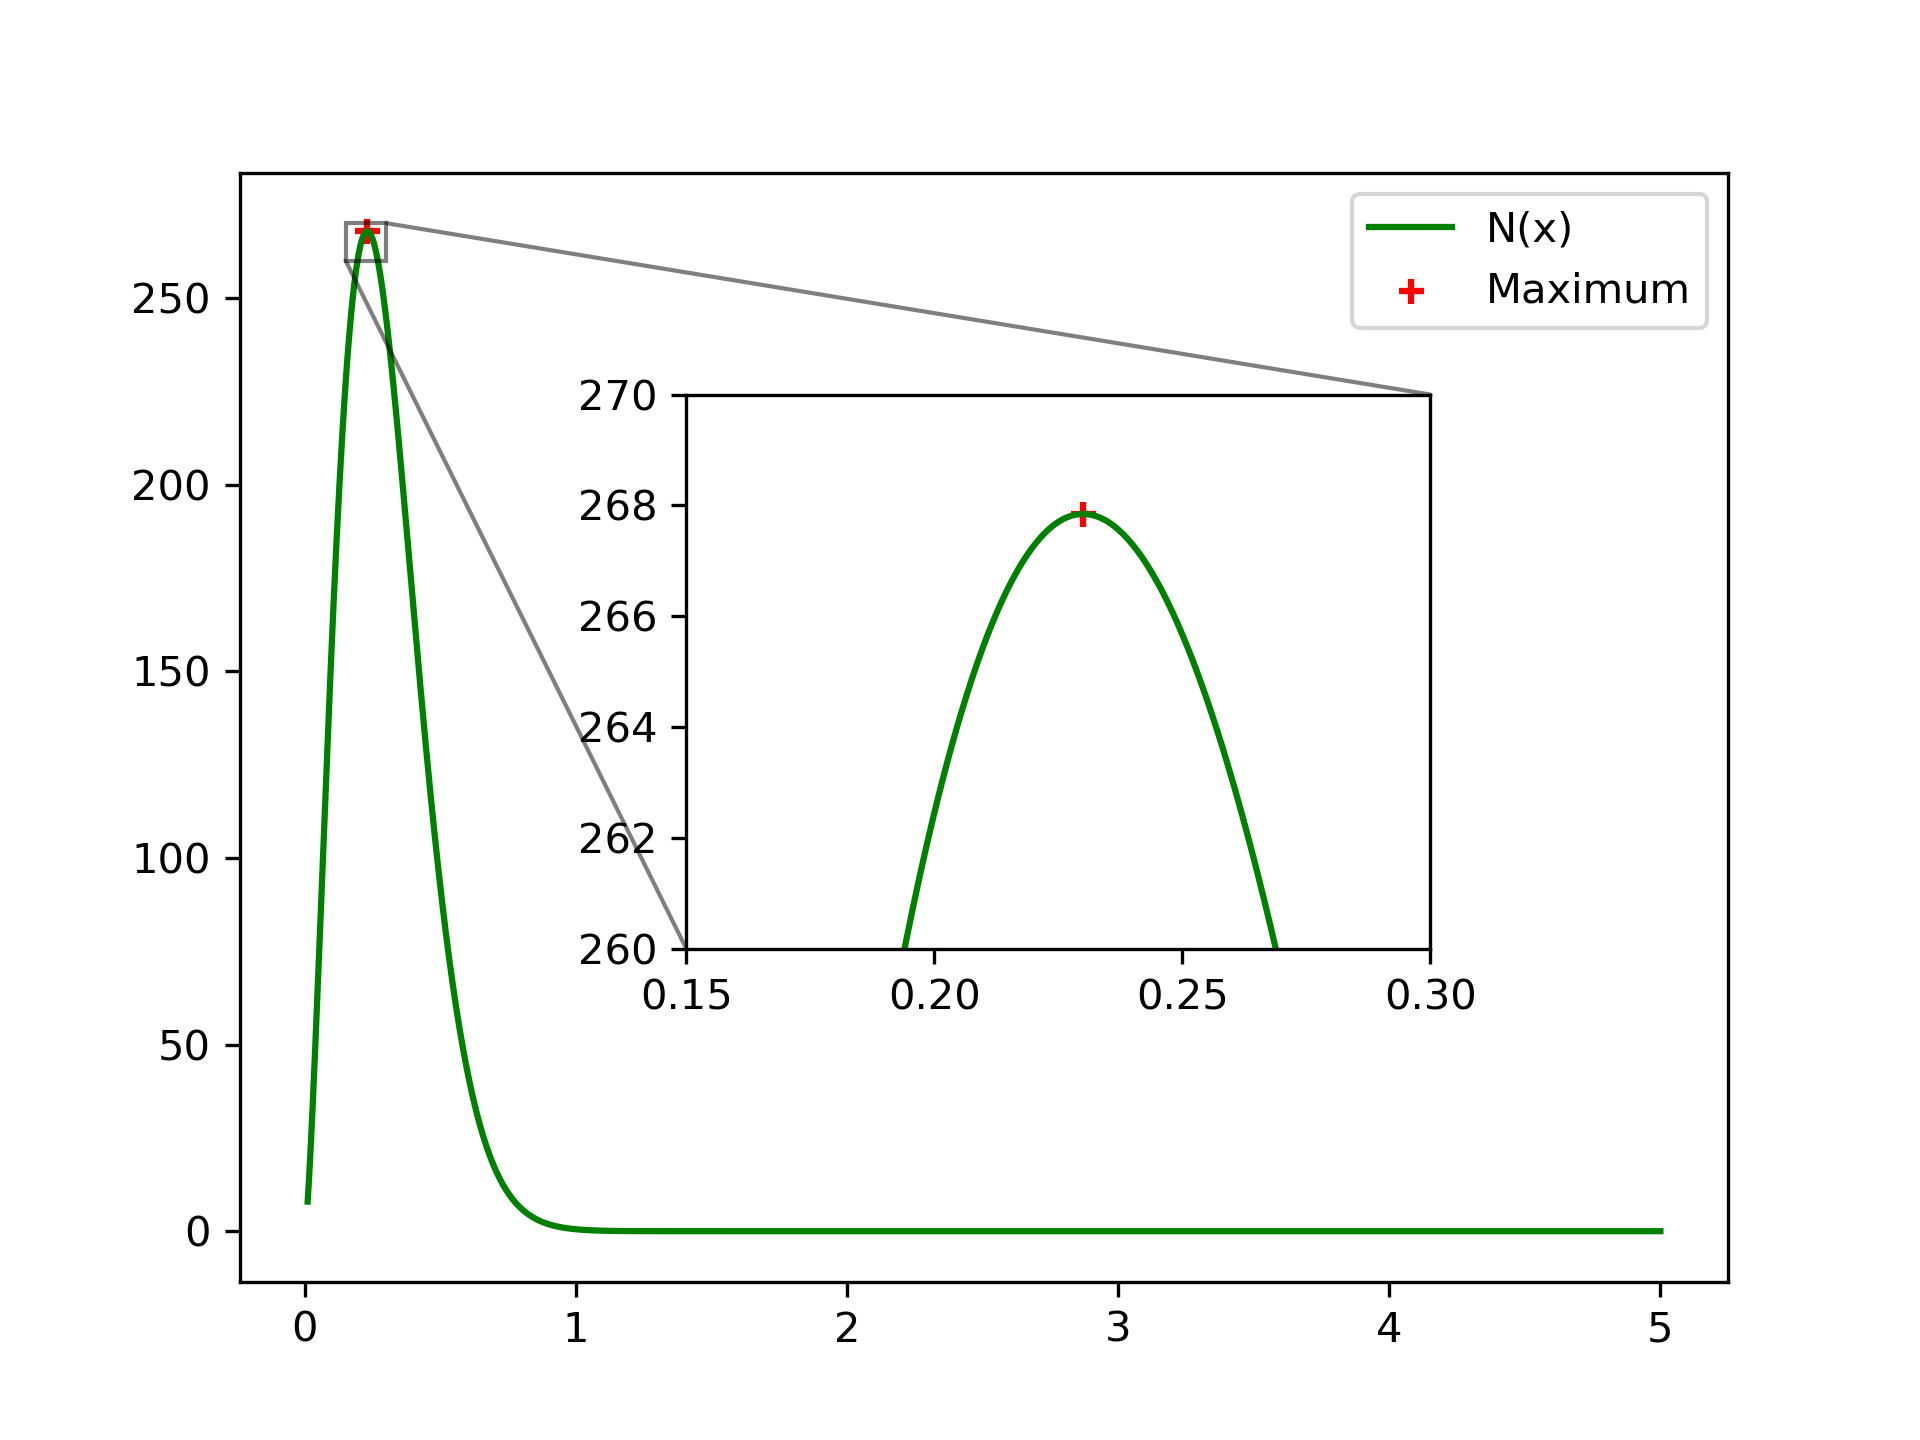
\includegraphics[width=.8\linewidth]{./plots/maximization.png}
  \caption{The number of galaxies as a function of x (radius relative to the virial radius). We also plot the position of the maximum value as it was calculated using the ``golden section search'' algorithm with the help of the ``bracketing a minimum'' algorithm.}
  \label{fig:max}
\end{figure}


\subsection{$\chi^2$ minimization}
\label{chap:chi}

For our next task, we want to use this model to fit some data. We have 5 different files containing haloes (in a certain halo mass bin) with variable numbers of satellites. The satellite galaxies are discrete objects and we, therefore, have a Poisson distribution. We can however fit the data using a $\chi^2$ minimization fit to find the values of the free parameters $a,\,b,\,c$.

We will perform a $\chi^2$ fit with the correct Poisson variance $\sigma^2 = \mu$. To do that we need to first bin our data. We chose 20 bins evenly distributed in real space. The reason we chose to work in real space and not in a logarithmic one was the fact that while we attempted to use both, our implementation worked much better in real space. This certainly has to do with our functions and the minimization algorithm that we used. 

To fit a model in a set of binned data using a $\chi^2$ minimization we use the following equation
\begin{equation}
  \label{eq:chi2}
  \chi^2 = \sum^{N-1}_{i=0}\frac{[y_i-\mu(x_i|p)]^2}{\sigma^2}=\sum^{N-1}_{i=0}\frac{[y_i-\mu(x|p)]^2}{\mu(x_i|p)^2}
\end{equation}
where $y_i$ is the observed binned data, $\mu(x|p)$ is the model mean at the middle of each bin, and $\sigma^2$ is the variance of the model which as we already discussed is equal to the model mean. 

In our problem we evaluate the model mean as follows:
\begin{equation}
  N_i=4\pi \int^{x_{i+1}}_{x_i} n(x) x^2 dx
\end{equation} 
which is essentially the integral over the length of each bin for our equation $N(x)$ which we previously discussed. It is important to note that as the values of $a,\,b,\,c$ change during minimization we need to calibrate $A$ so that the following equation is always true:
\begin{equation}
  4\pi \int^{5}_{x=0} n(x) x^2 dx = \langle N_{sat} \rangle
\end{equation}

To accomplish all that we implement many different functions. First of all, we have a ``readfile'' function that can give us a list of all the satellite galaxy radii and also the number of haloes in each file. We then define the ``f\_n'' function which is the $N(x)$ function defined in a way that doesn't require an open formula for it to be integrated. We also use a ``trapezoid'' function to enable us to calculate the integral. We also experimented with using a function that utilizes the Romberg integration algorithm, with no improvement on the final performance, so we decided to use the more simple trapezoid algorithm. All these integration routines were implemented in a previous assignment. 

To perform the minimization we implemented the downhill simplex algorithm in our function ``simplex\_3d''. This implementation is mainly for 3-dimensional spaces as it requires four initial points to work with (N+1). These four points can be visualized as a triangular prism in the 3d plane of our parameters. We propose a new point by reflecting the worst point on the surface that is defined by the other 3 points. If our new point has the best estimate overall we expand once more and check if there is still an improvement. Otherwise, we check if our new point is an improvement over our worst point and we then accept our new point. If neither of these two cases is met, we propose a new point by contracting instead of reflecting, which means that we search inwards instead of outwards. If this didn't also give us a better result we will shrink our initial prism. We iterate for a number of max iterations and return our best guess or we can stop early if the fractional range in our function evaluation gets sufficiently small. 

We then define the ``chisquare'' function which is the one we want to minimize. The function takes a list of the three parameters we try to evaluate, the counts of the binned data and the edges of each bin. We also input $ \langle N_{sat} \rangle $. We then calculate $A$ for the specific values of $a,\, b,\, c$ and loop over all bins to calculate the $\chi^2$ sum as we defined in \Cref{eq:chi2}.

We also define one final function to handle the plotting of the binned data with the best-fitted model. 

\lstinputlisting{chisquare.py}

In the main part of our code, we first want to read the data from the text files. We then bin the data using the numpy routine with ``density=True'' to normalize it. We also calculate $ \langle N_{sat} \rangle $ for each of our data files. Because we are working with normalized distributions our $ \langle N_{sat} \rangle $ is the number of galaxies in each file divided by the number of haloes. After that, we want to minimize our $\chi^2$ function for each data file and get the best estimates of $a,\, b,\, c$. The next part of the script is just for plotting and printing the values we want. Before plotting we need to calculate the correct value of $A$ for the specific data file and the values of the parameters.  

\lstinputlisting{output/chisquare.txt}

In the output of our script, we can see the values of $ \langle N_{sat} \rangle,\, a,\, b,\, c,\, \chi^2 $ for each data file. From \Cref{fig:chi-fit} we can see that our fitting was successful in all five datasets. The fitted model is falling on top of the bins as we would expect. This becomes even more clear when we plot in real space instead of log space. These plots can be found in \Cref{fig:chi-fit-app}.

\begin{figure}[H]
  \centering
  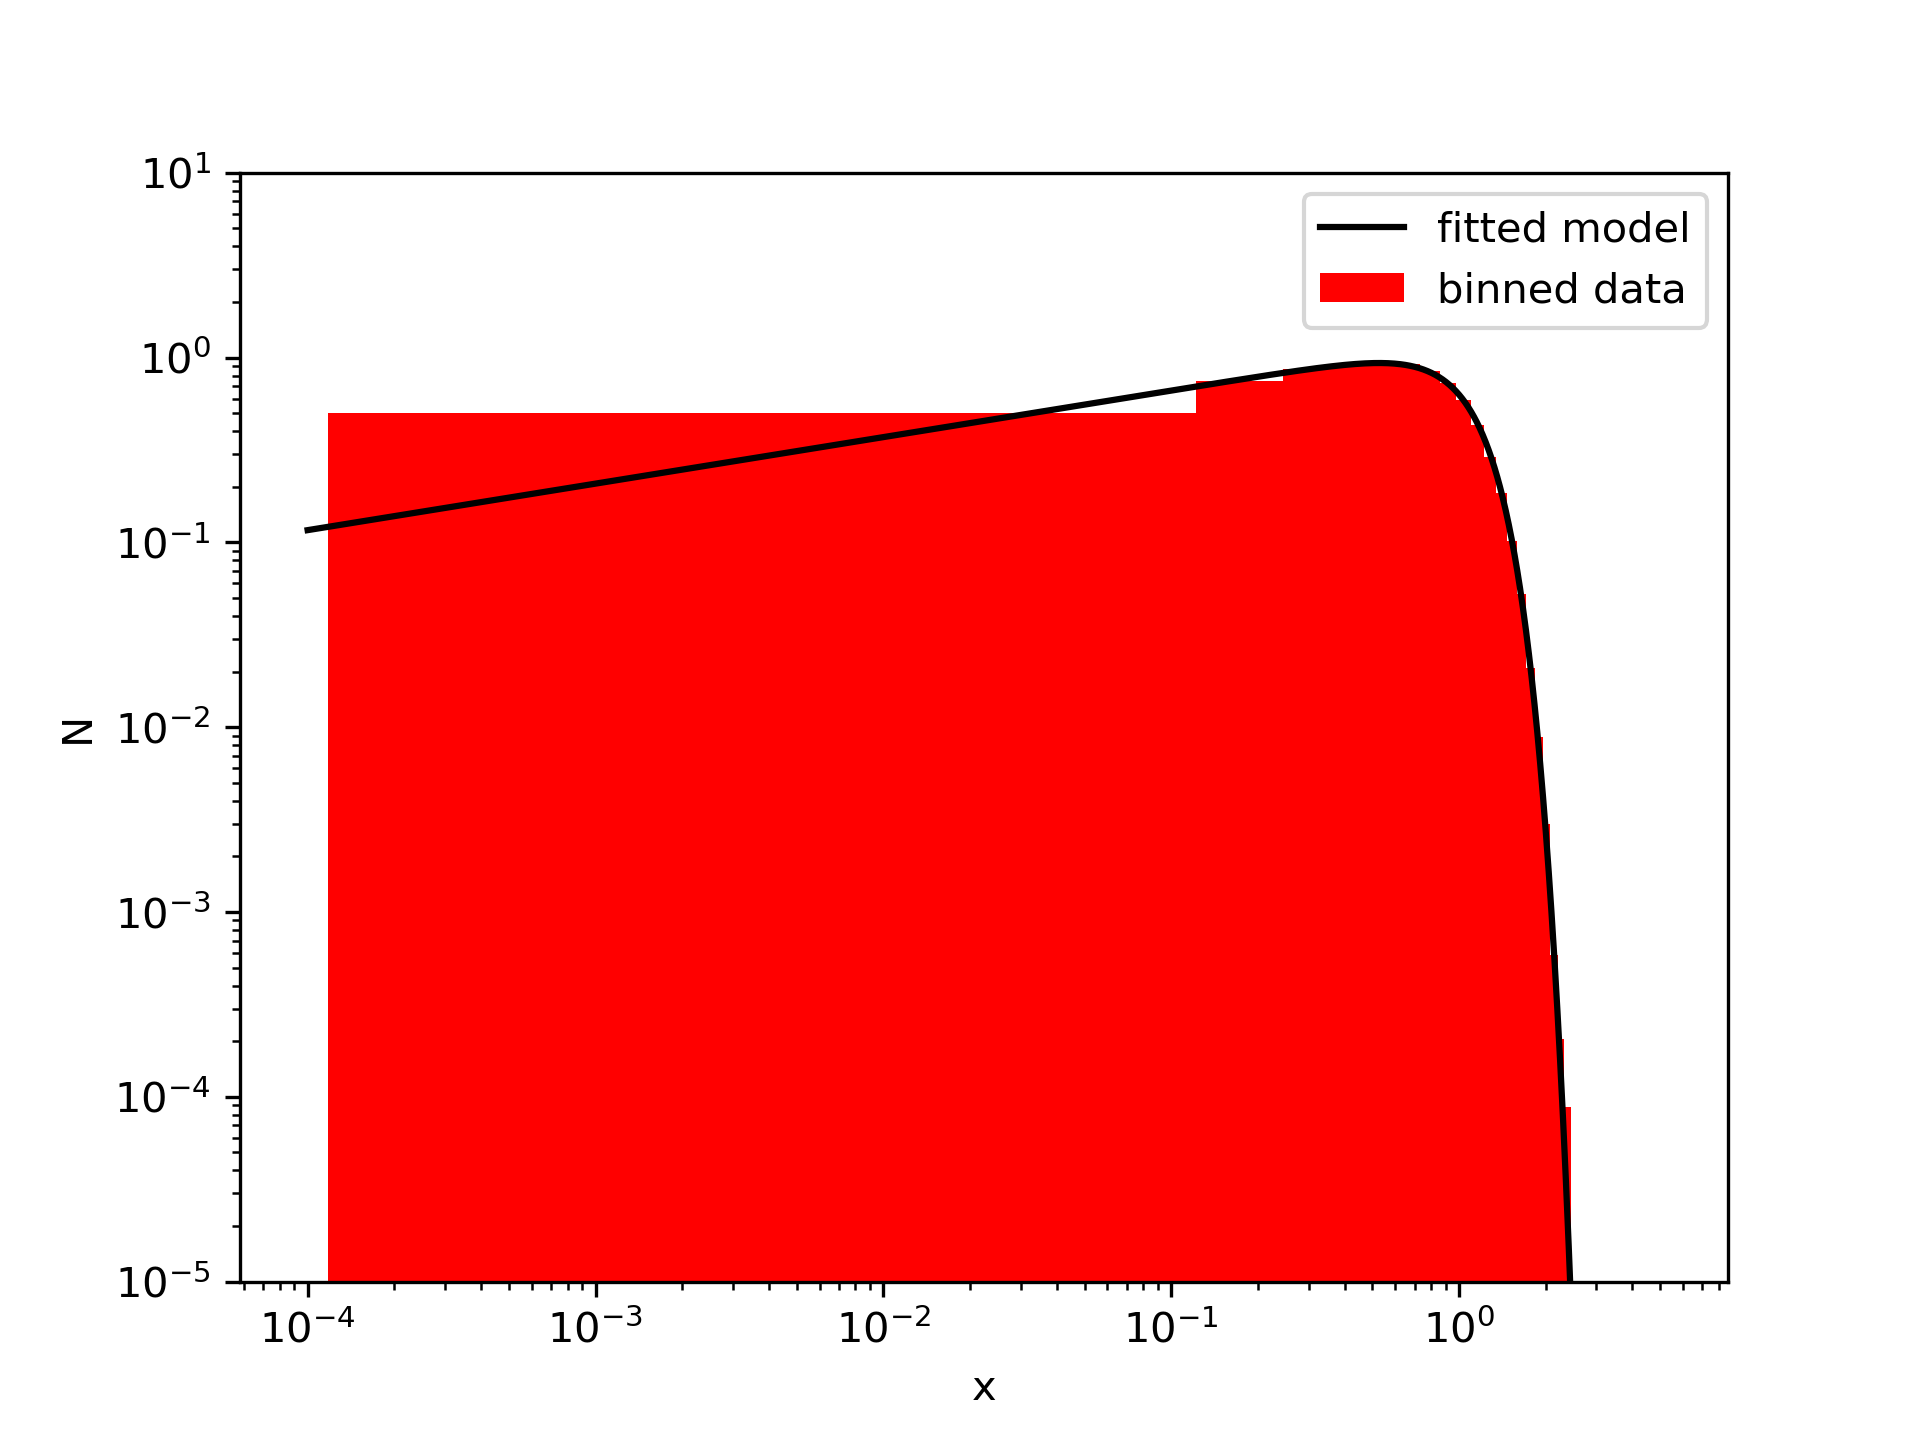
\includegraphics[width=.48\linewidth]{./plots/chi-fit1.png}
  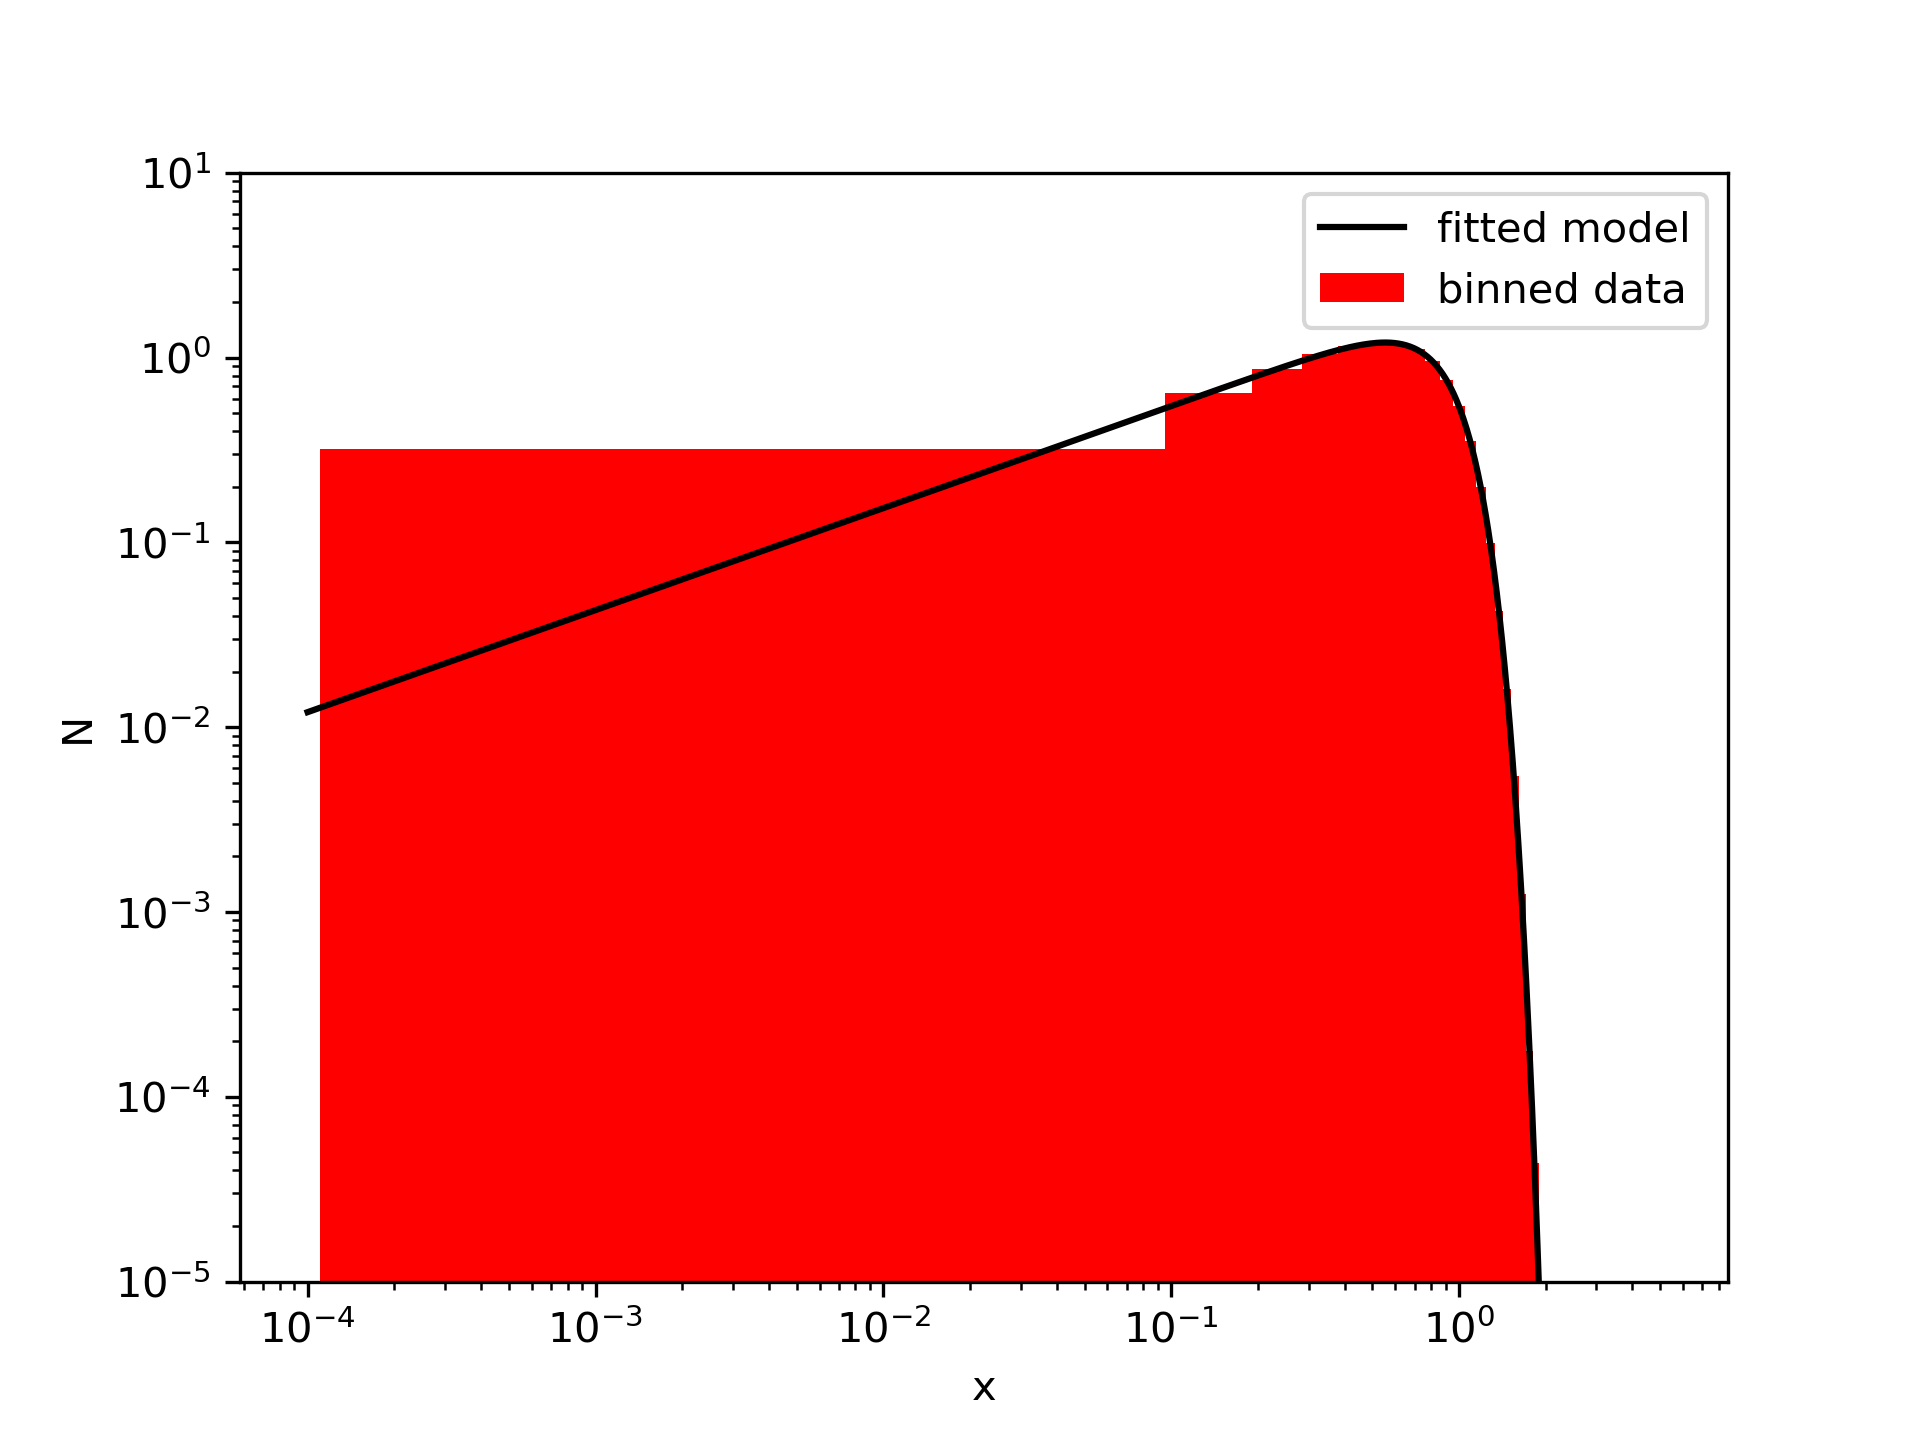
\includegraphics[width=.48\linewidth]{./plots/chi-fit2.png}
  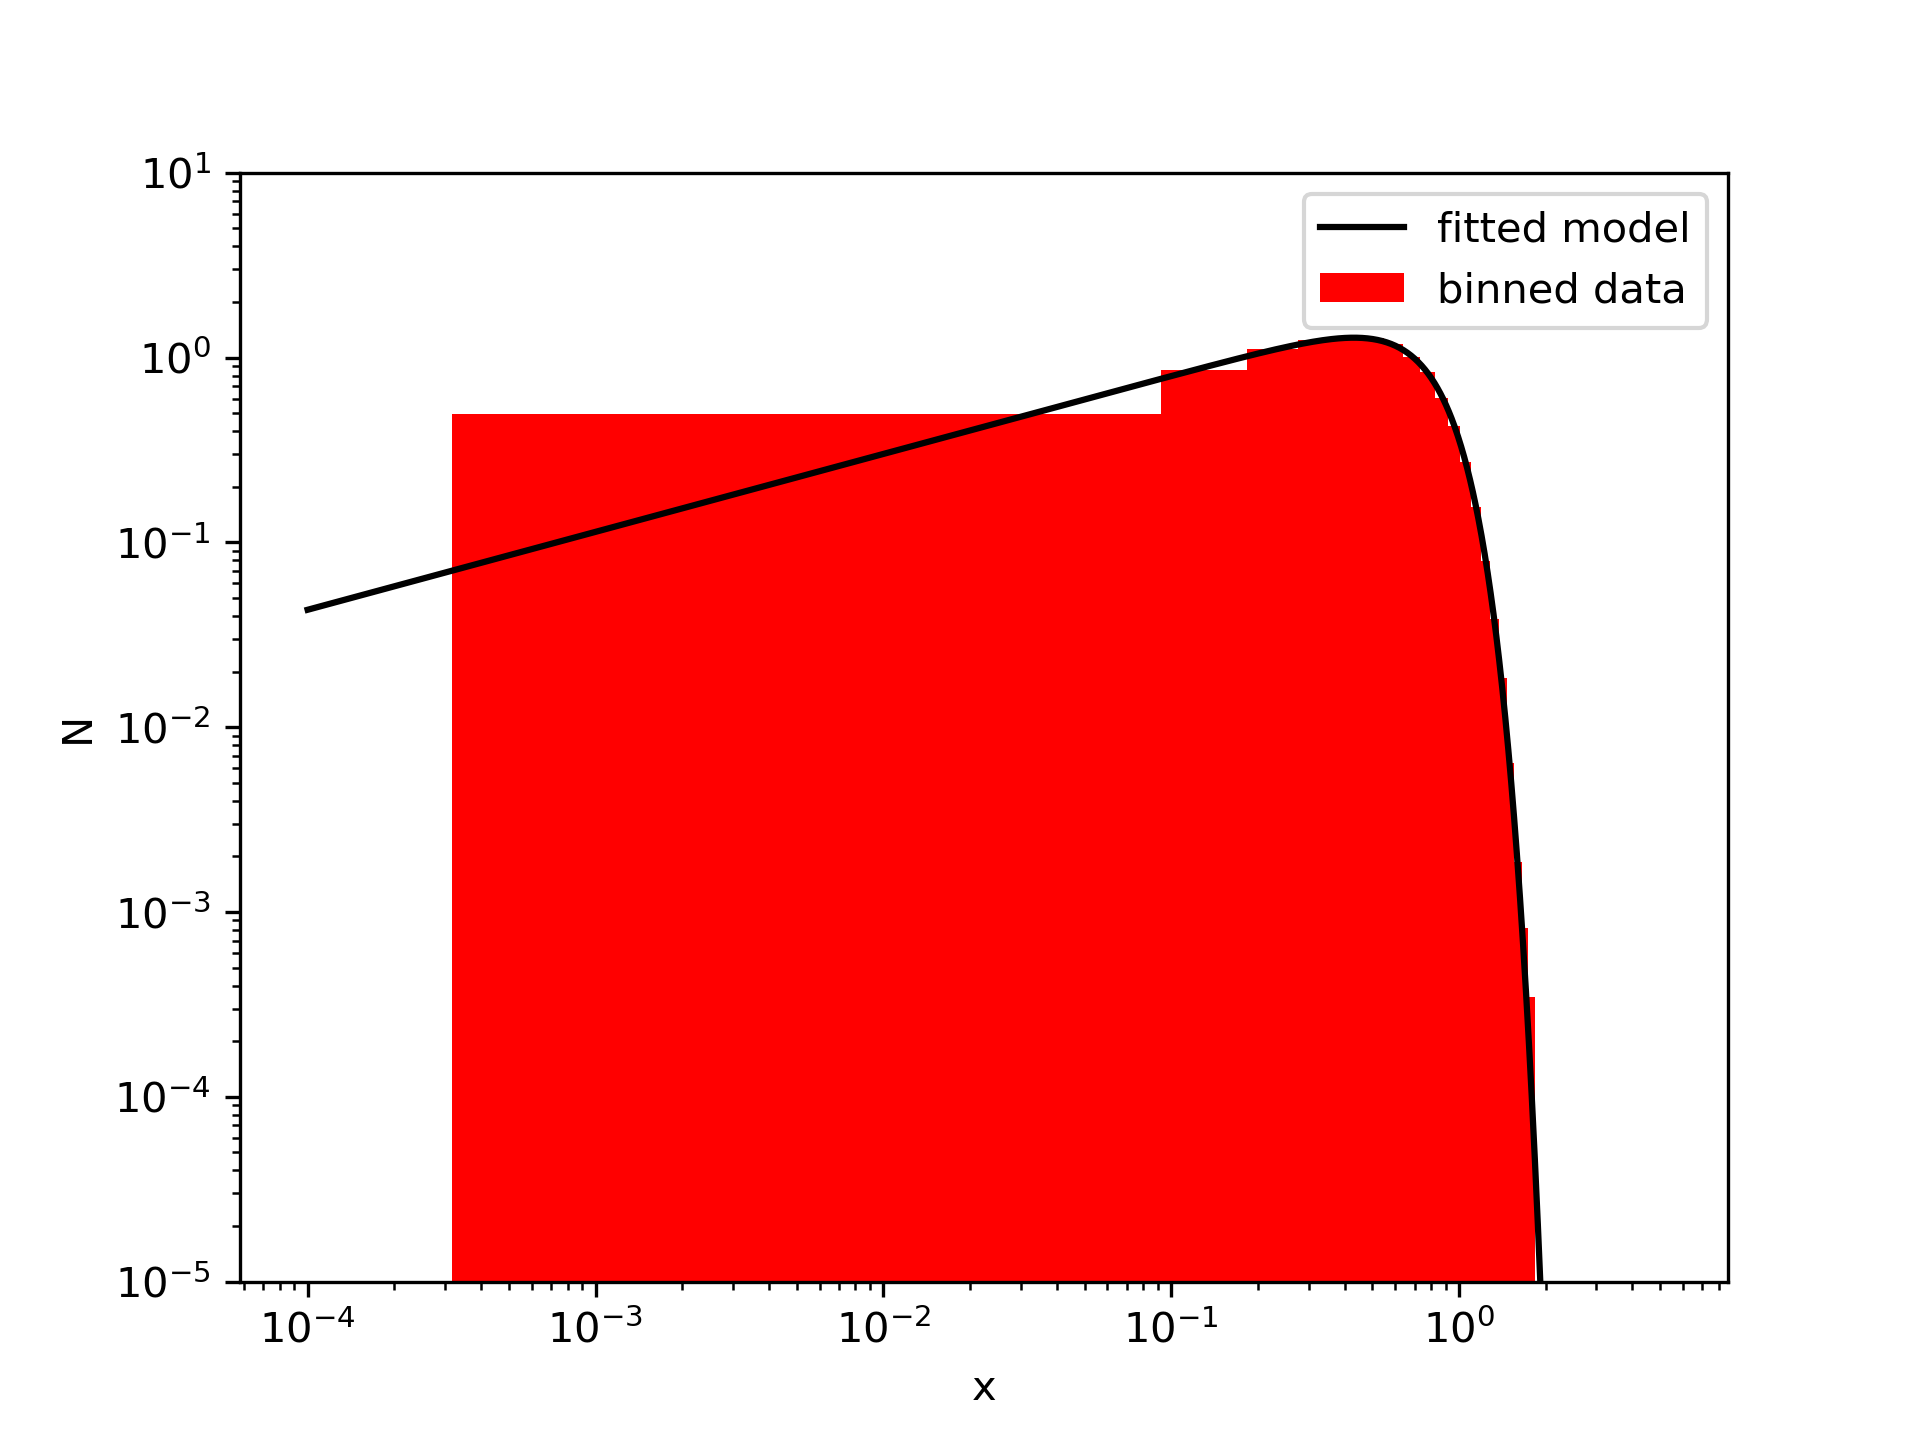
\includegraphics[width=.48\linewidth]{./plots/chi-fit3.png}
  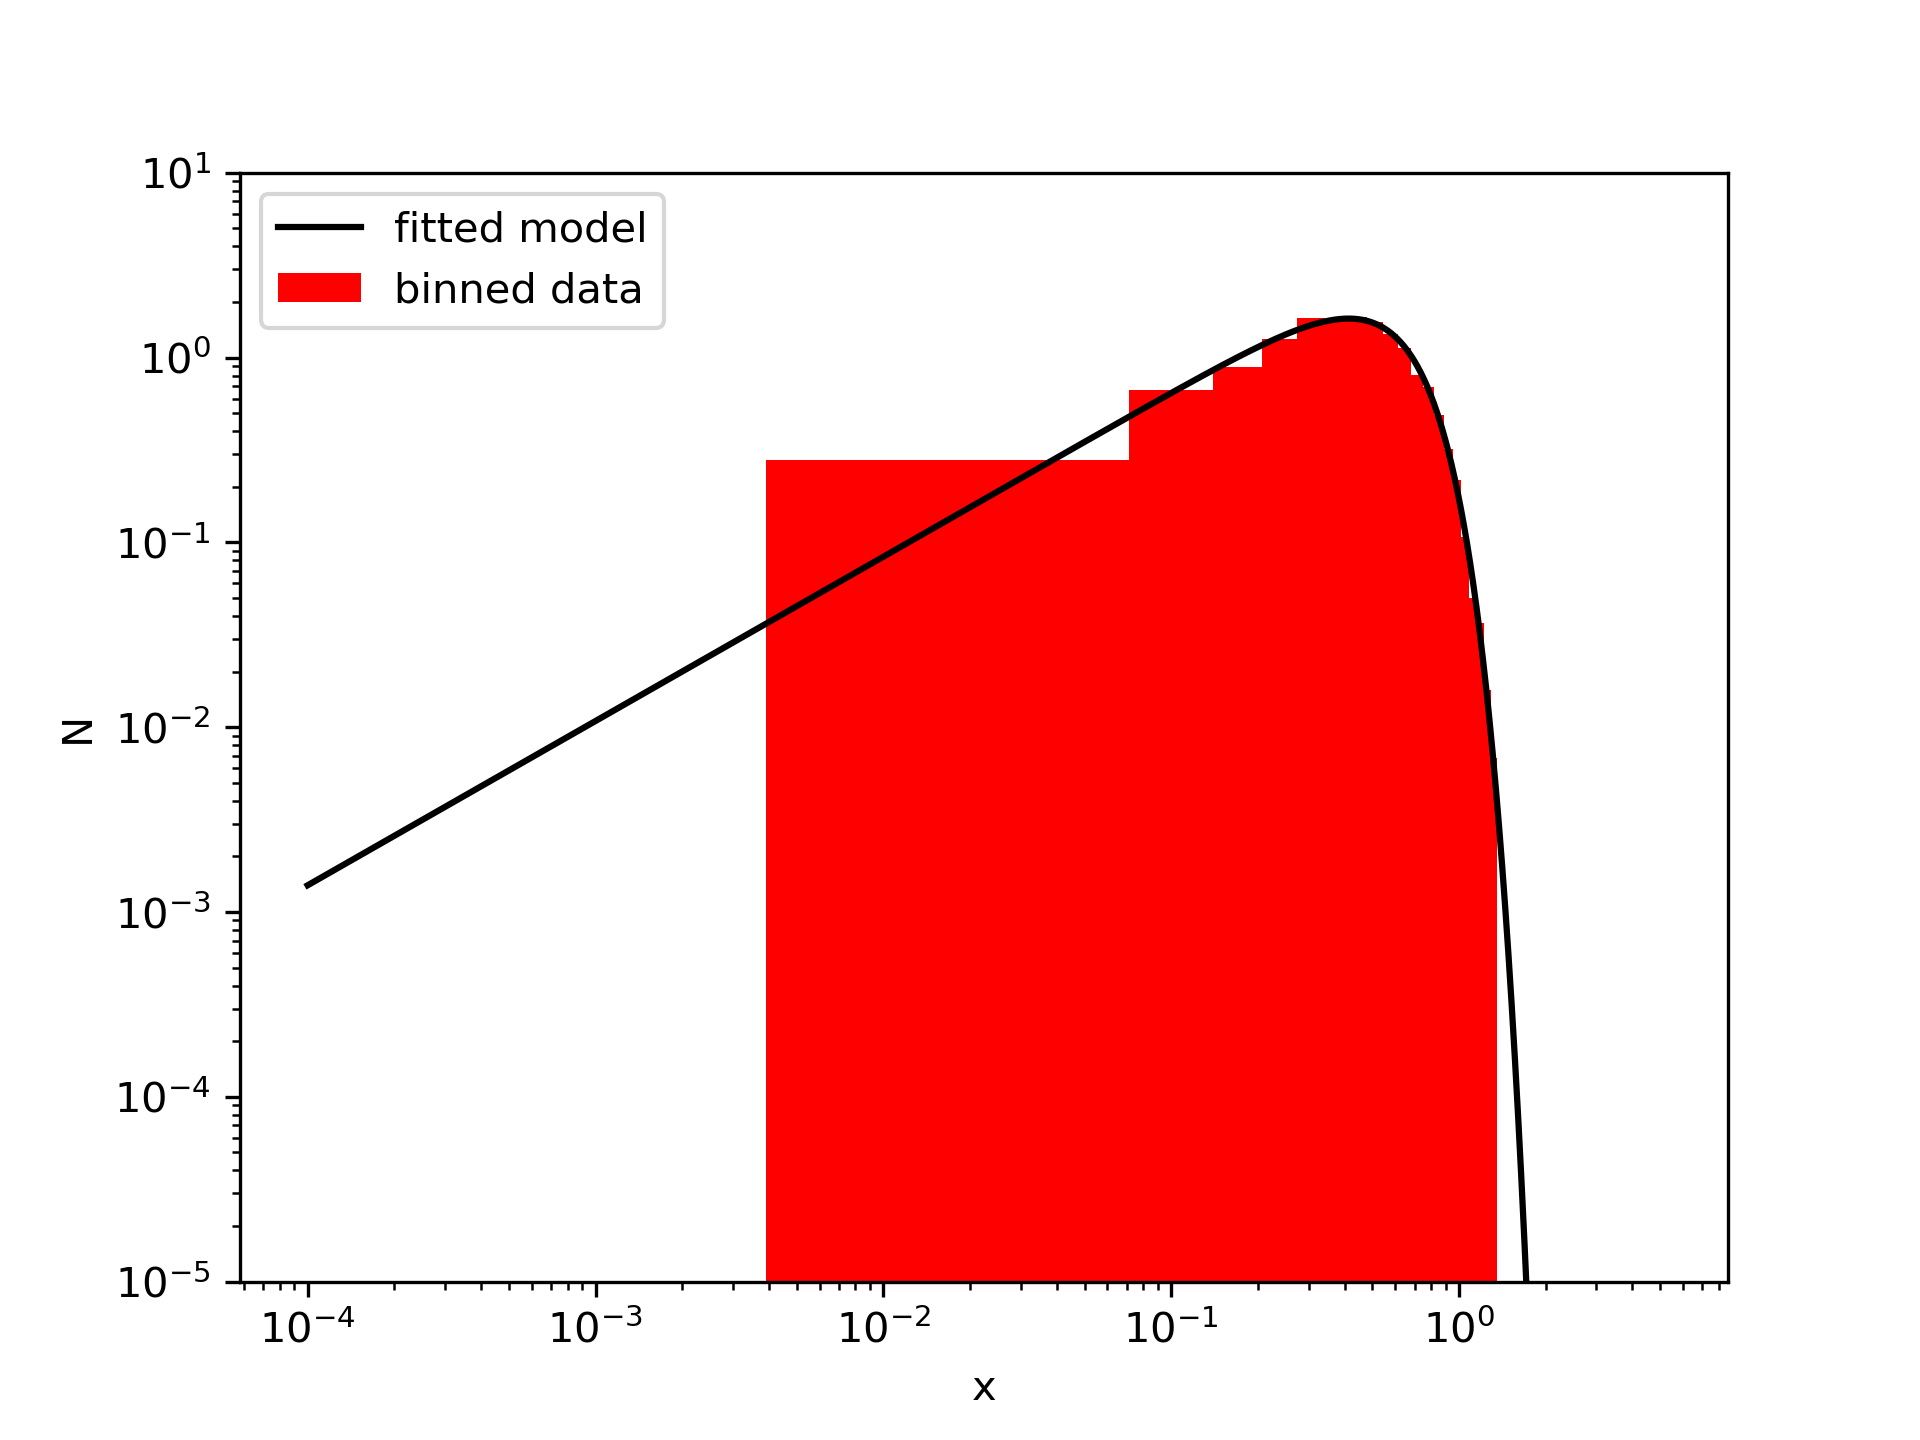
\includegraphics[width=.48\linewidth]{./plots/chi-fit4.png}
  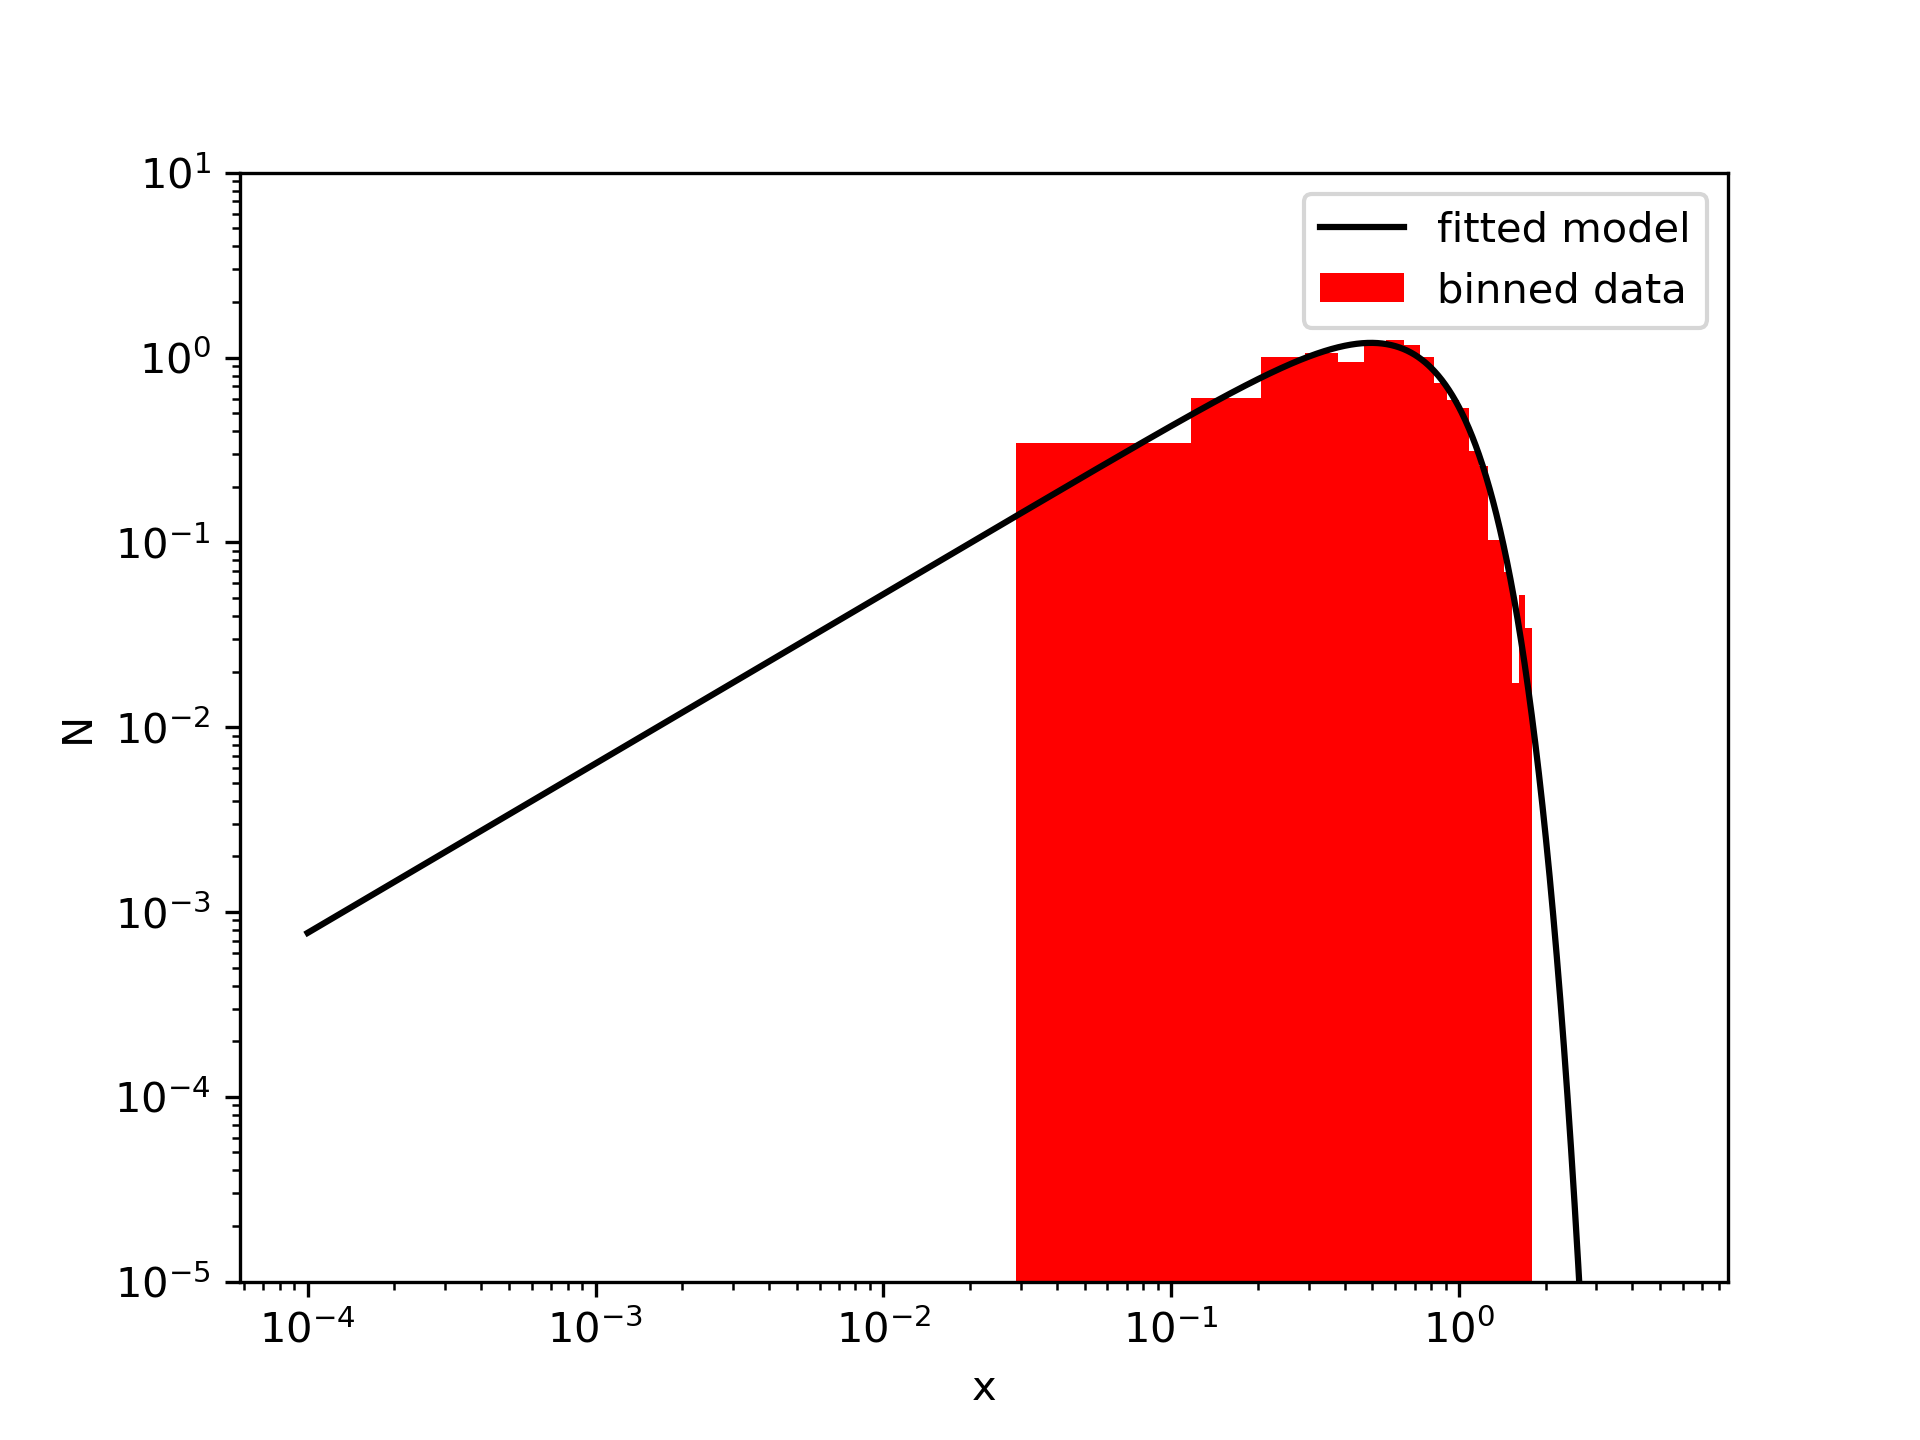
\includegraphics[width=.48\linewidth]{./plots/chi-fit5.png}
  \caption{The binned data with the best-fit model for each dataset. The plot is in logarithmic scale for both the x and the y axis. To fit the model we minimized $\chi^2$ function. We can see that the model greatly fits our data in all five cases. }
  \label{fig:chi-fit}
\end{figure}


\subsection{Poisson log-likelihood}
\label{chap:poisson}

In this task, we want to switch from minimizing the $\chi^2$ function to the more appropriate one for our problem Poisson log-likelihood. The negative log-likelihood that we want to minimize can be expressed by:
\begin{equation}
  -\ln(L(p))=-\sum^{N-1}_{i=0}[y_i \ln(\mu(x_i|p))-\mu(x_i|p)- \ln(y_i!)]
\end{equation}
where $y_i$ is the observed binned data, $\mu(x|p)$ is the model mean at the middle of each bin. We notice that the last term is not dependent on our parameters $p$ and can therefore be disregarded during the minimization process. 

We implement our function ``loglikelihood'' which calculates the negative log-likelihood as it was described by inputting the observed binned data and the model. We then use the same minimization process that was described and implemented in \Cref{chap:chi} by calling the ``simplex\_3d'' function to minimize the log-likelihood. 

\lstinputlisting{likelihood.py}

The code outputs the values of $a,\,b,\,c$ for each dataset and also the negative log-likelihood that was minimized. We also create plots to visualize the performance of our fitting. As we can see in \Cref{fig:pois-fit} the fitting is good as our model greatly matches the binned data. This becomes even more clear when we plot in real space as is shown in \Cref{fig:pois-fit-app}

\begin{figure}[H]
  \centering
  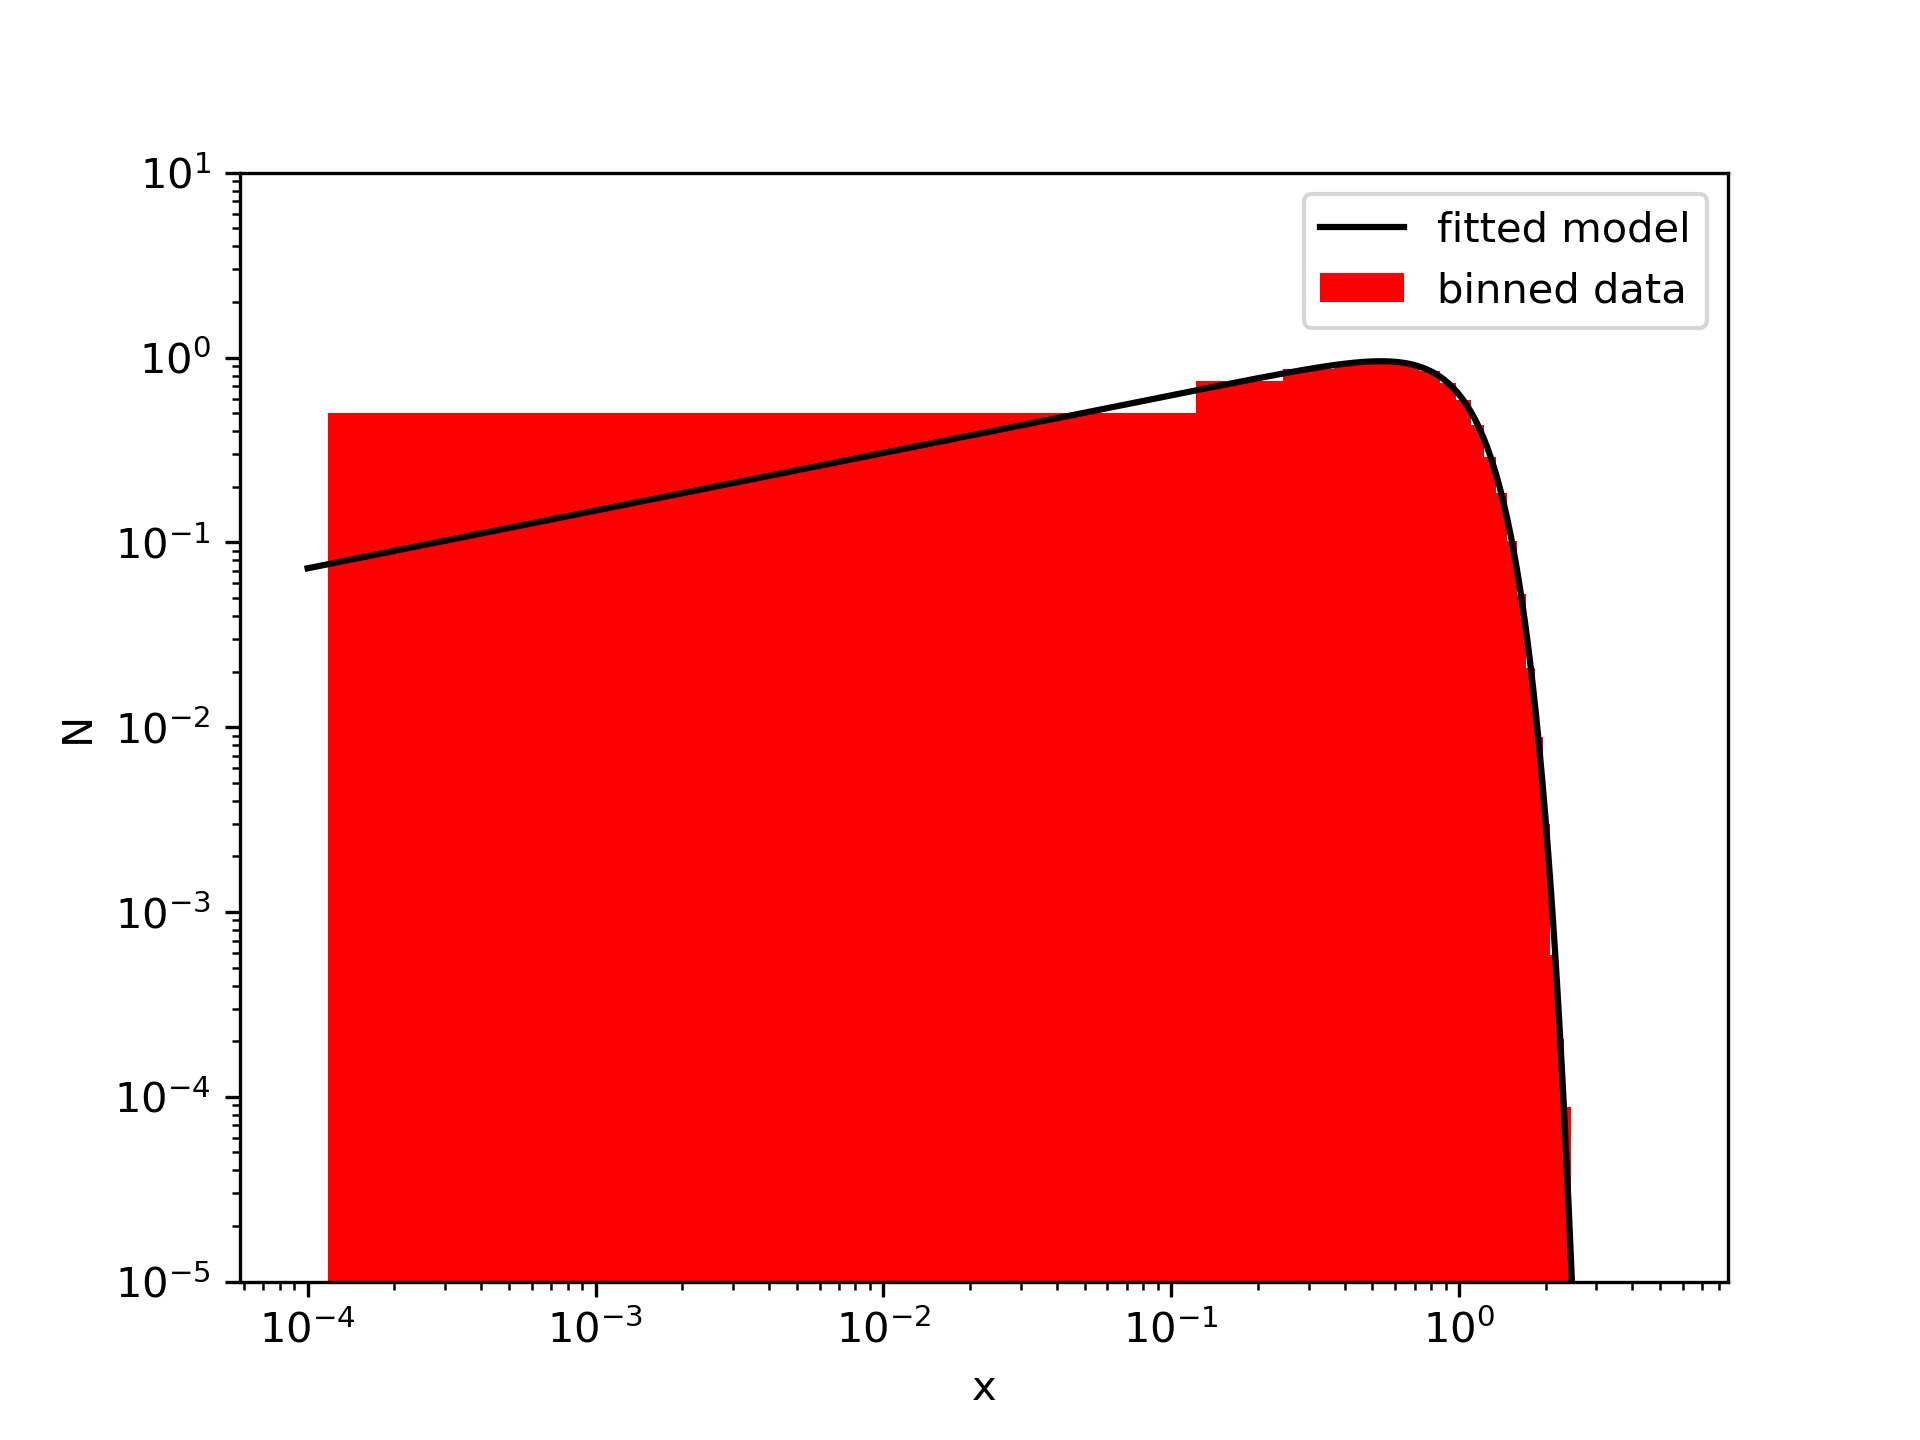
\includegraphics[width=.48\linewidth]{./plots/pois-fit1.png}
  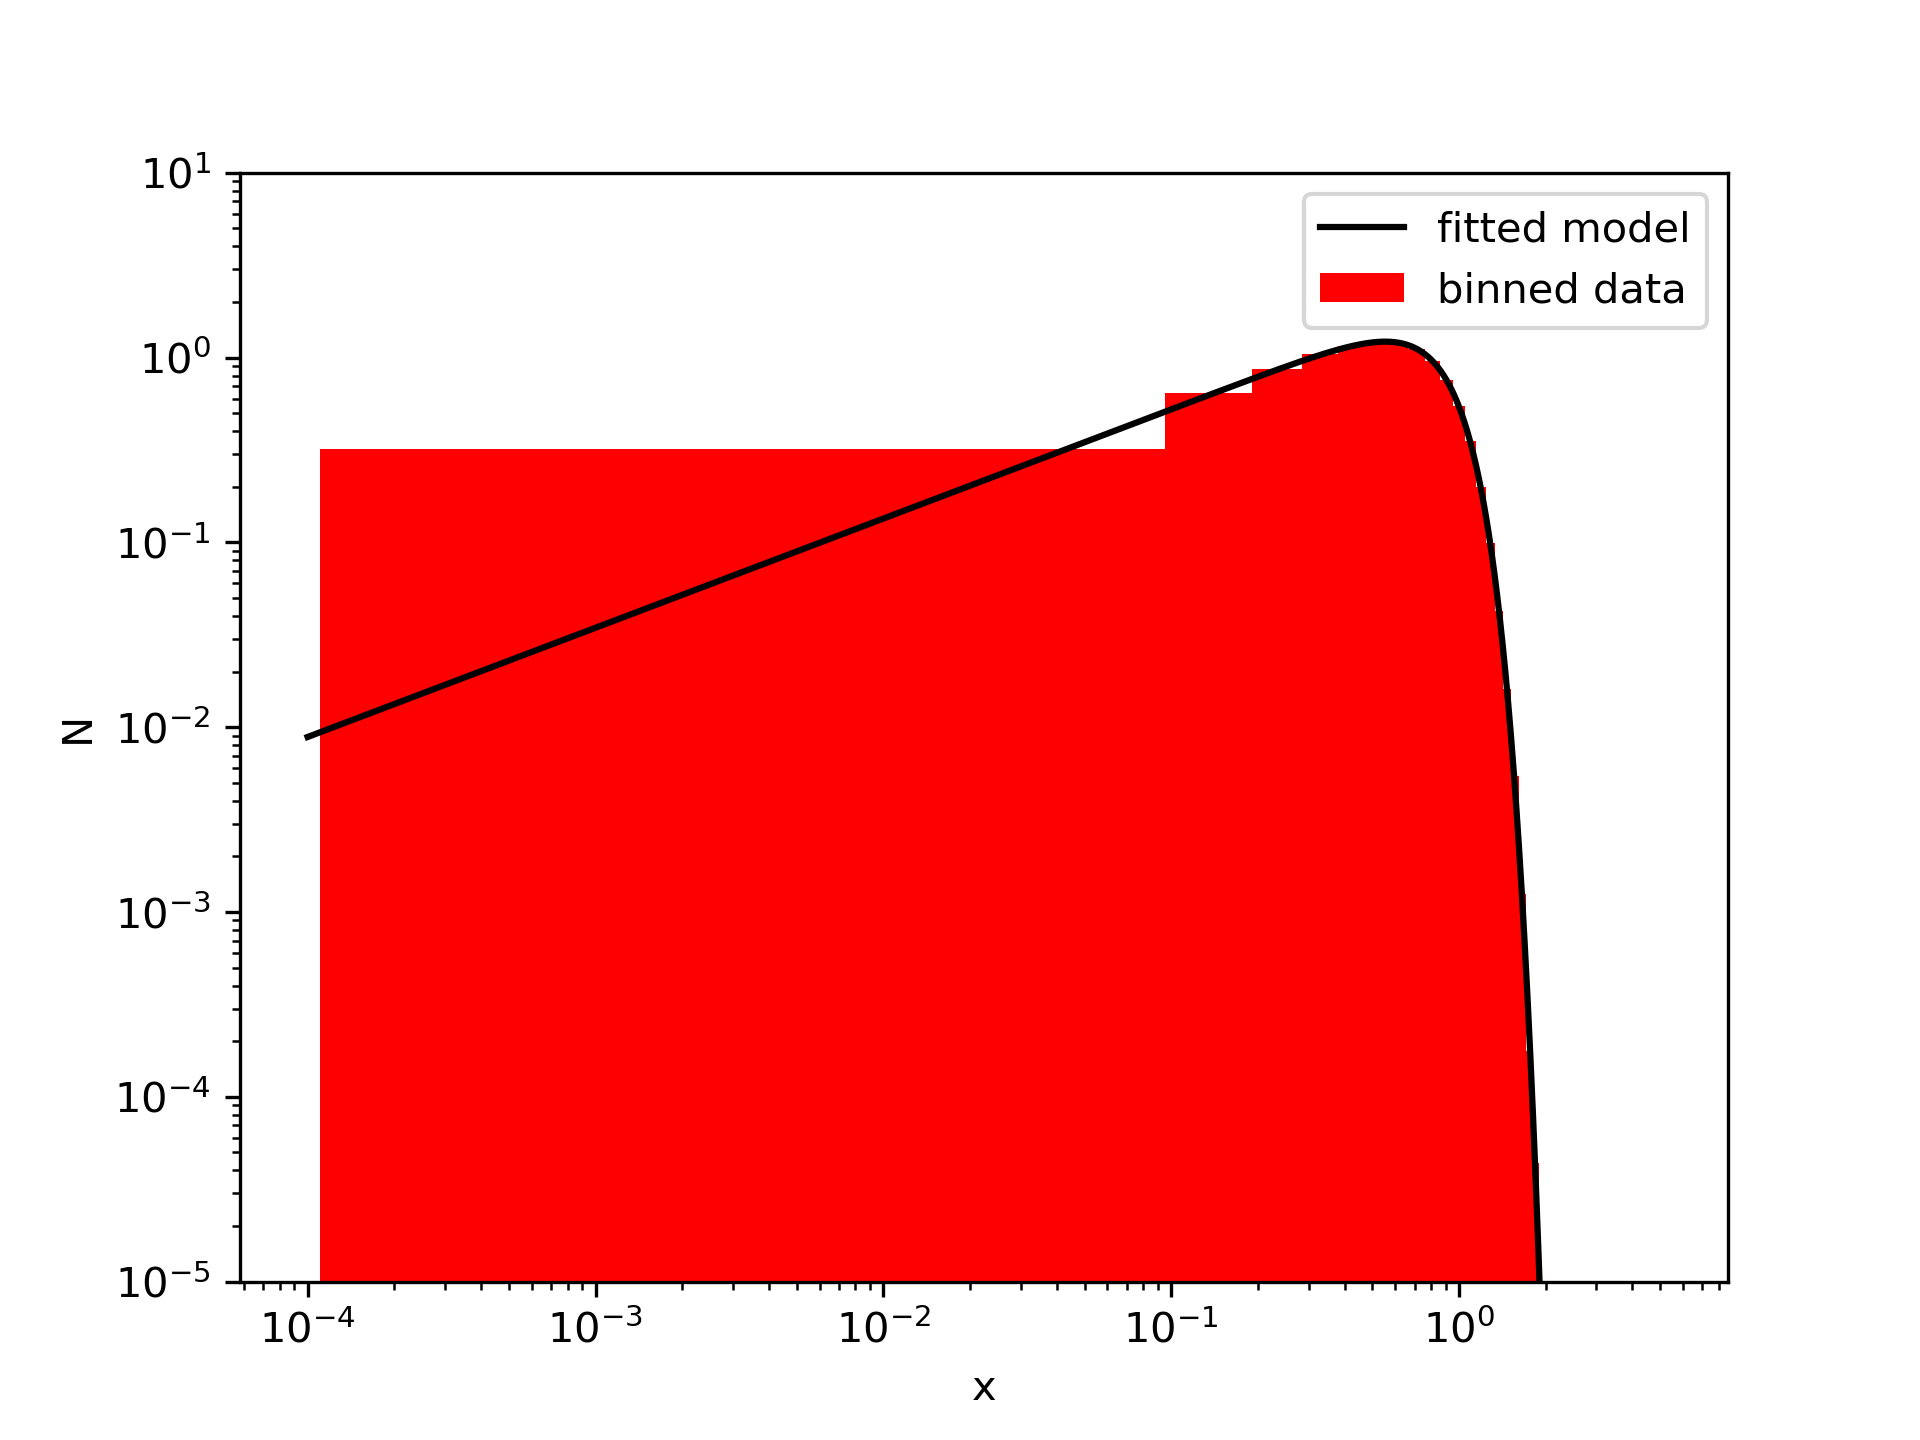
\includegraphics[width=.48\linewidth]{./plots/pois-fit2.png}
  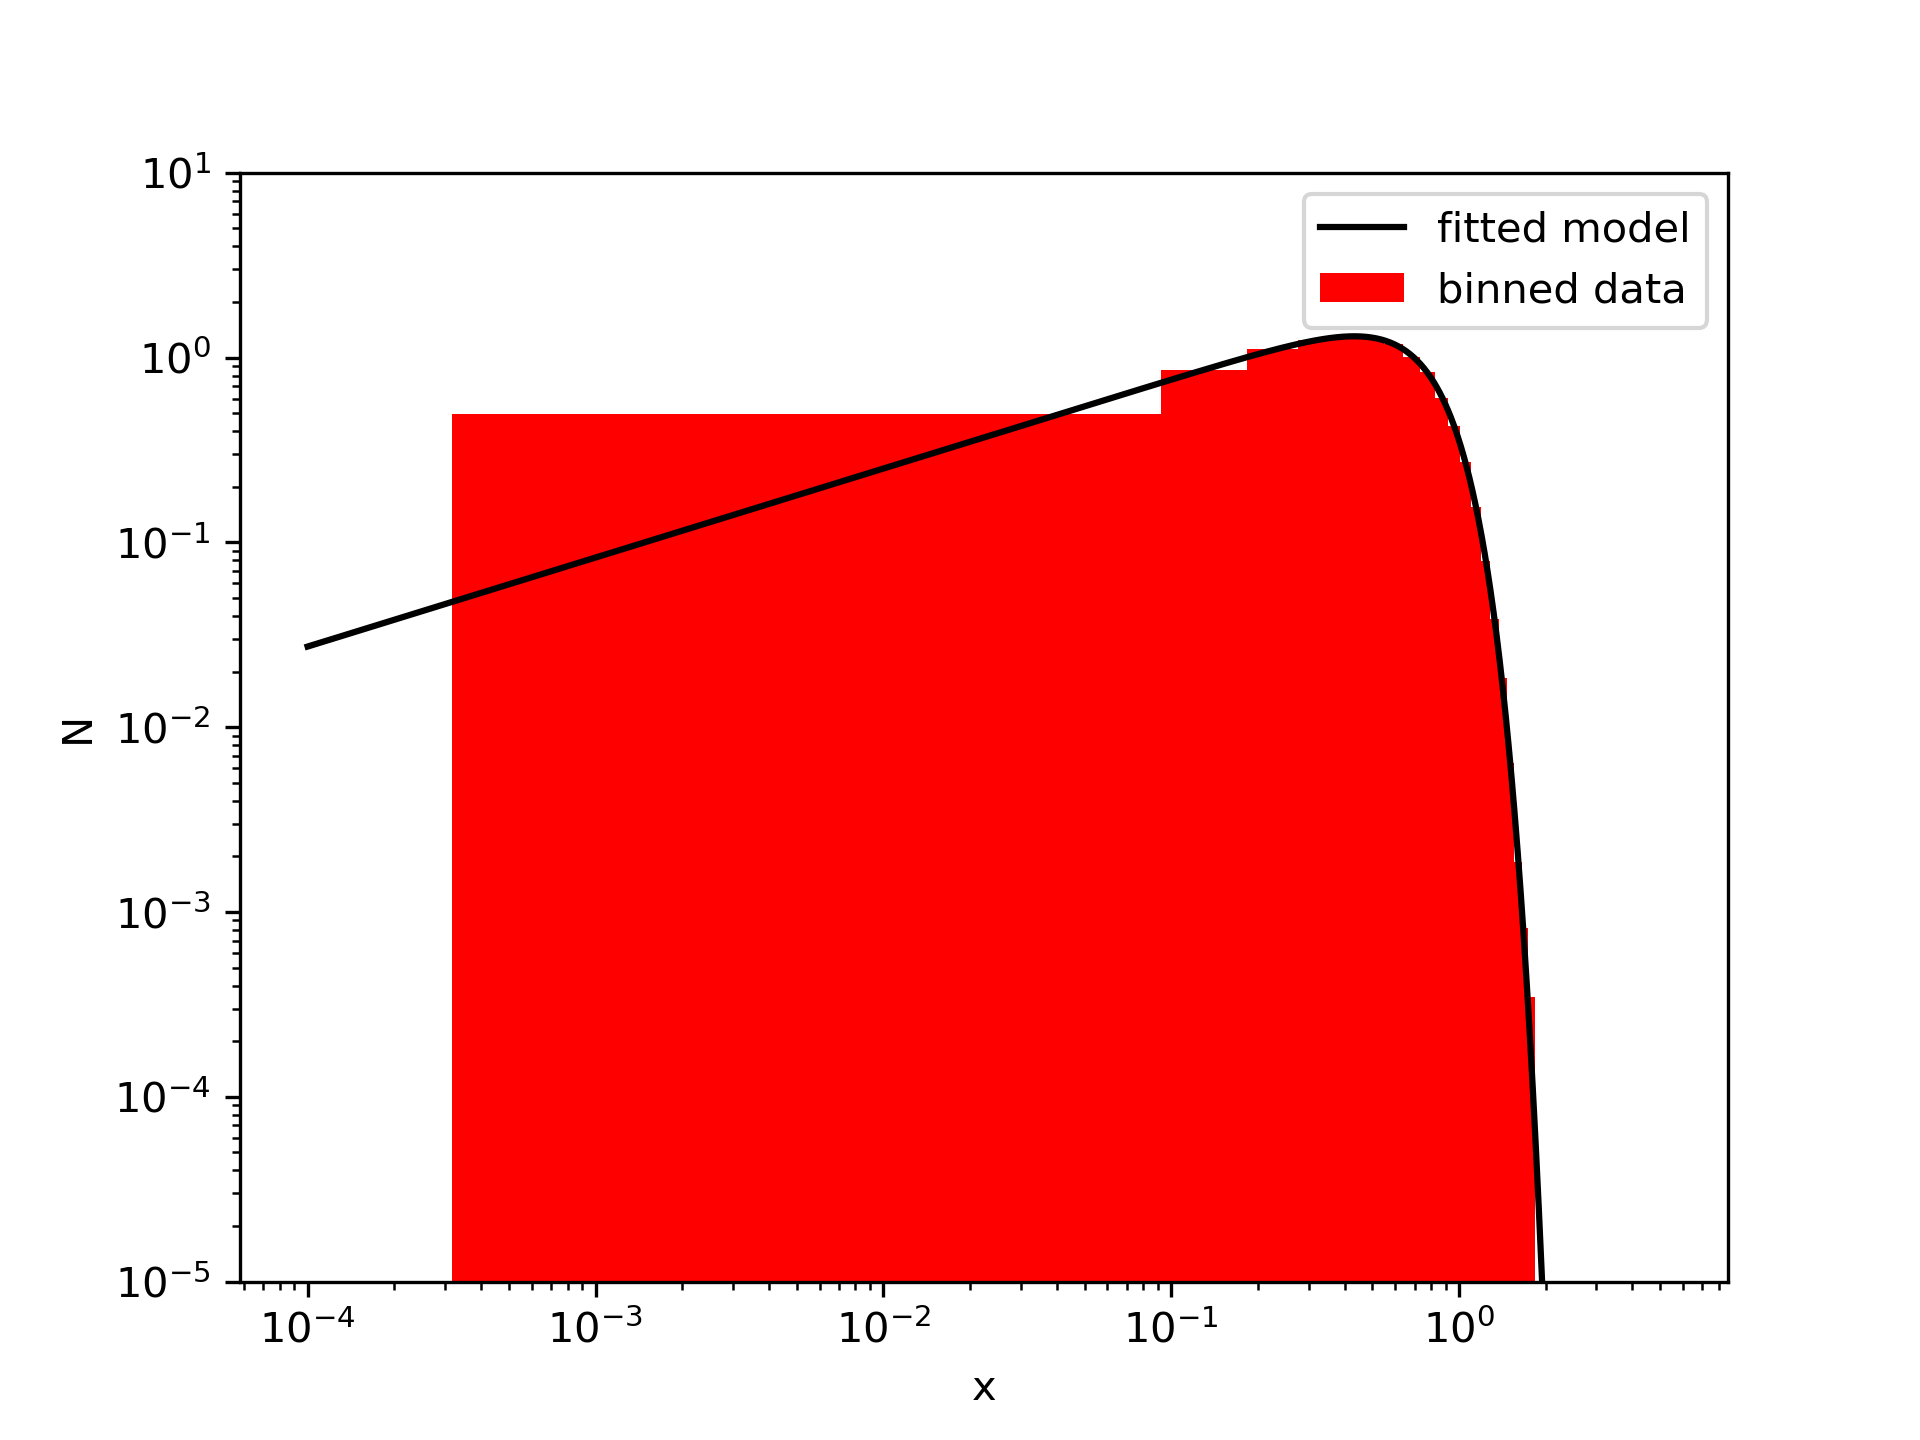
\includegraphics[width=.48\linewidth]{./plots/pois-fit3.png}
  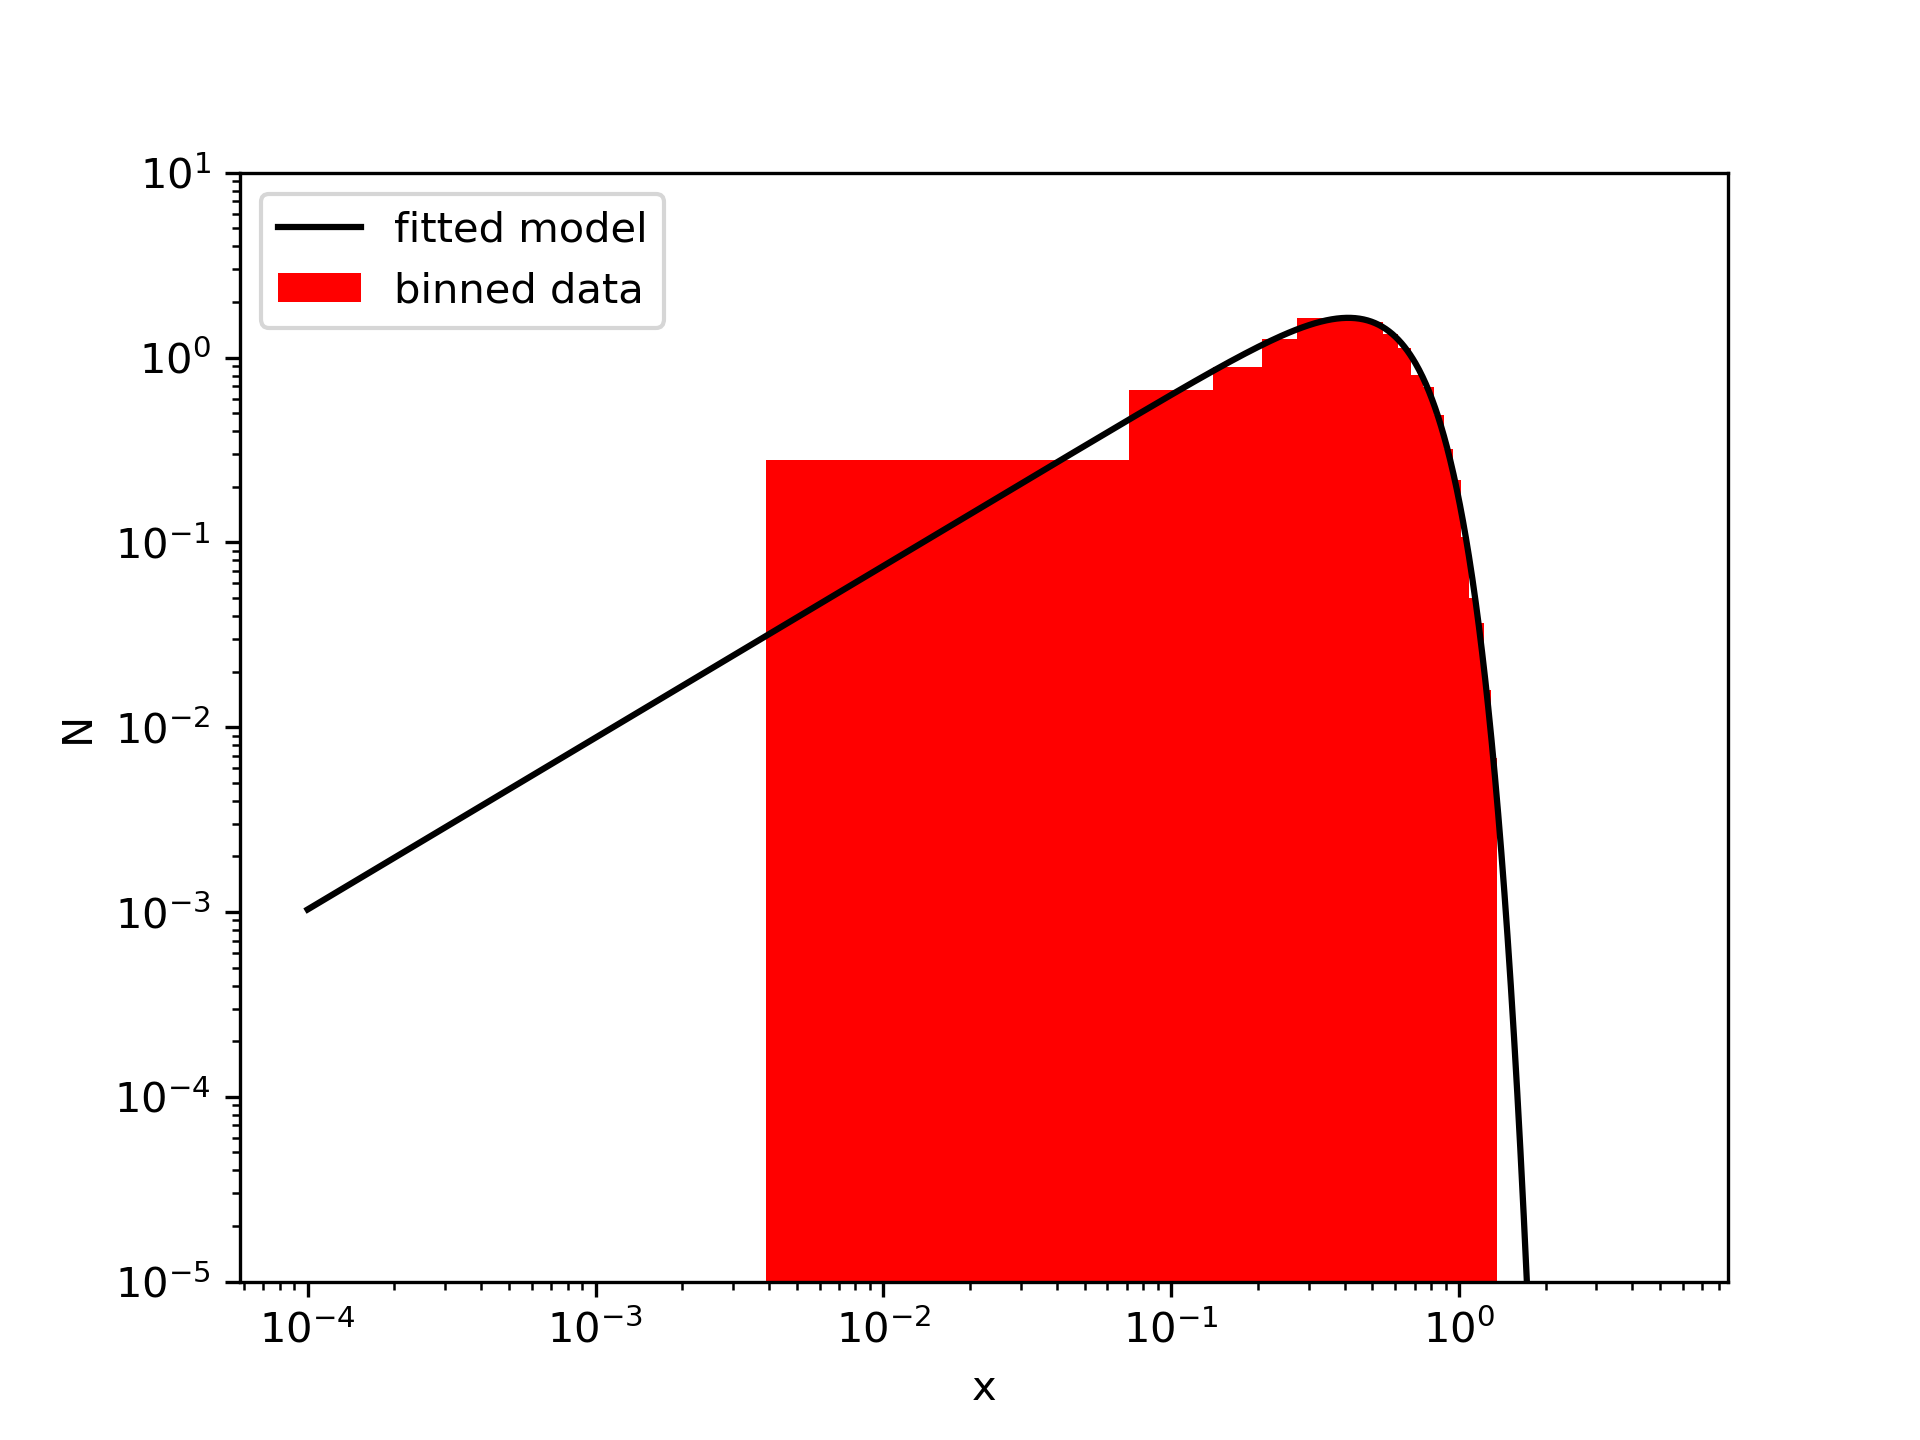
\includegraphics[width=.48\linewidth]{./plots/pois-fit4.png}
  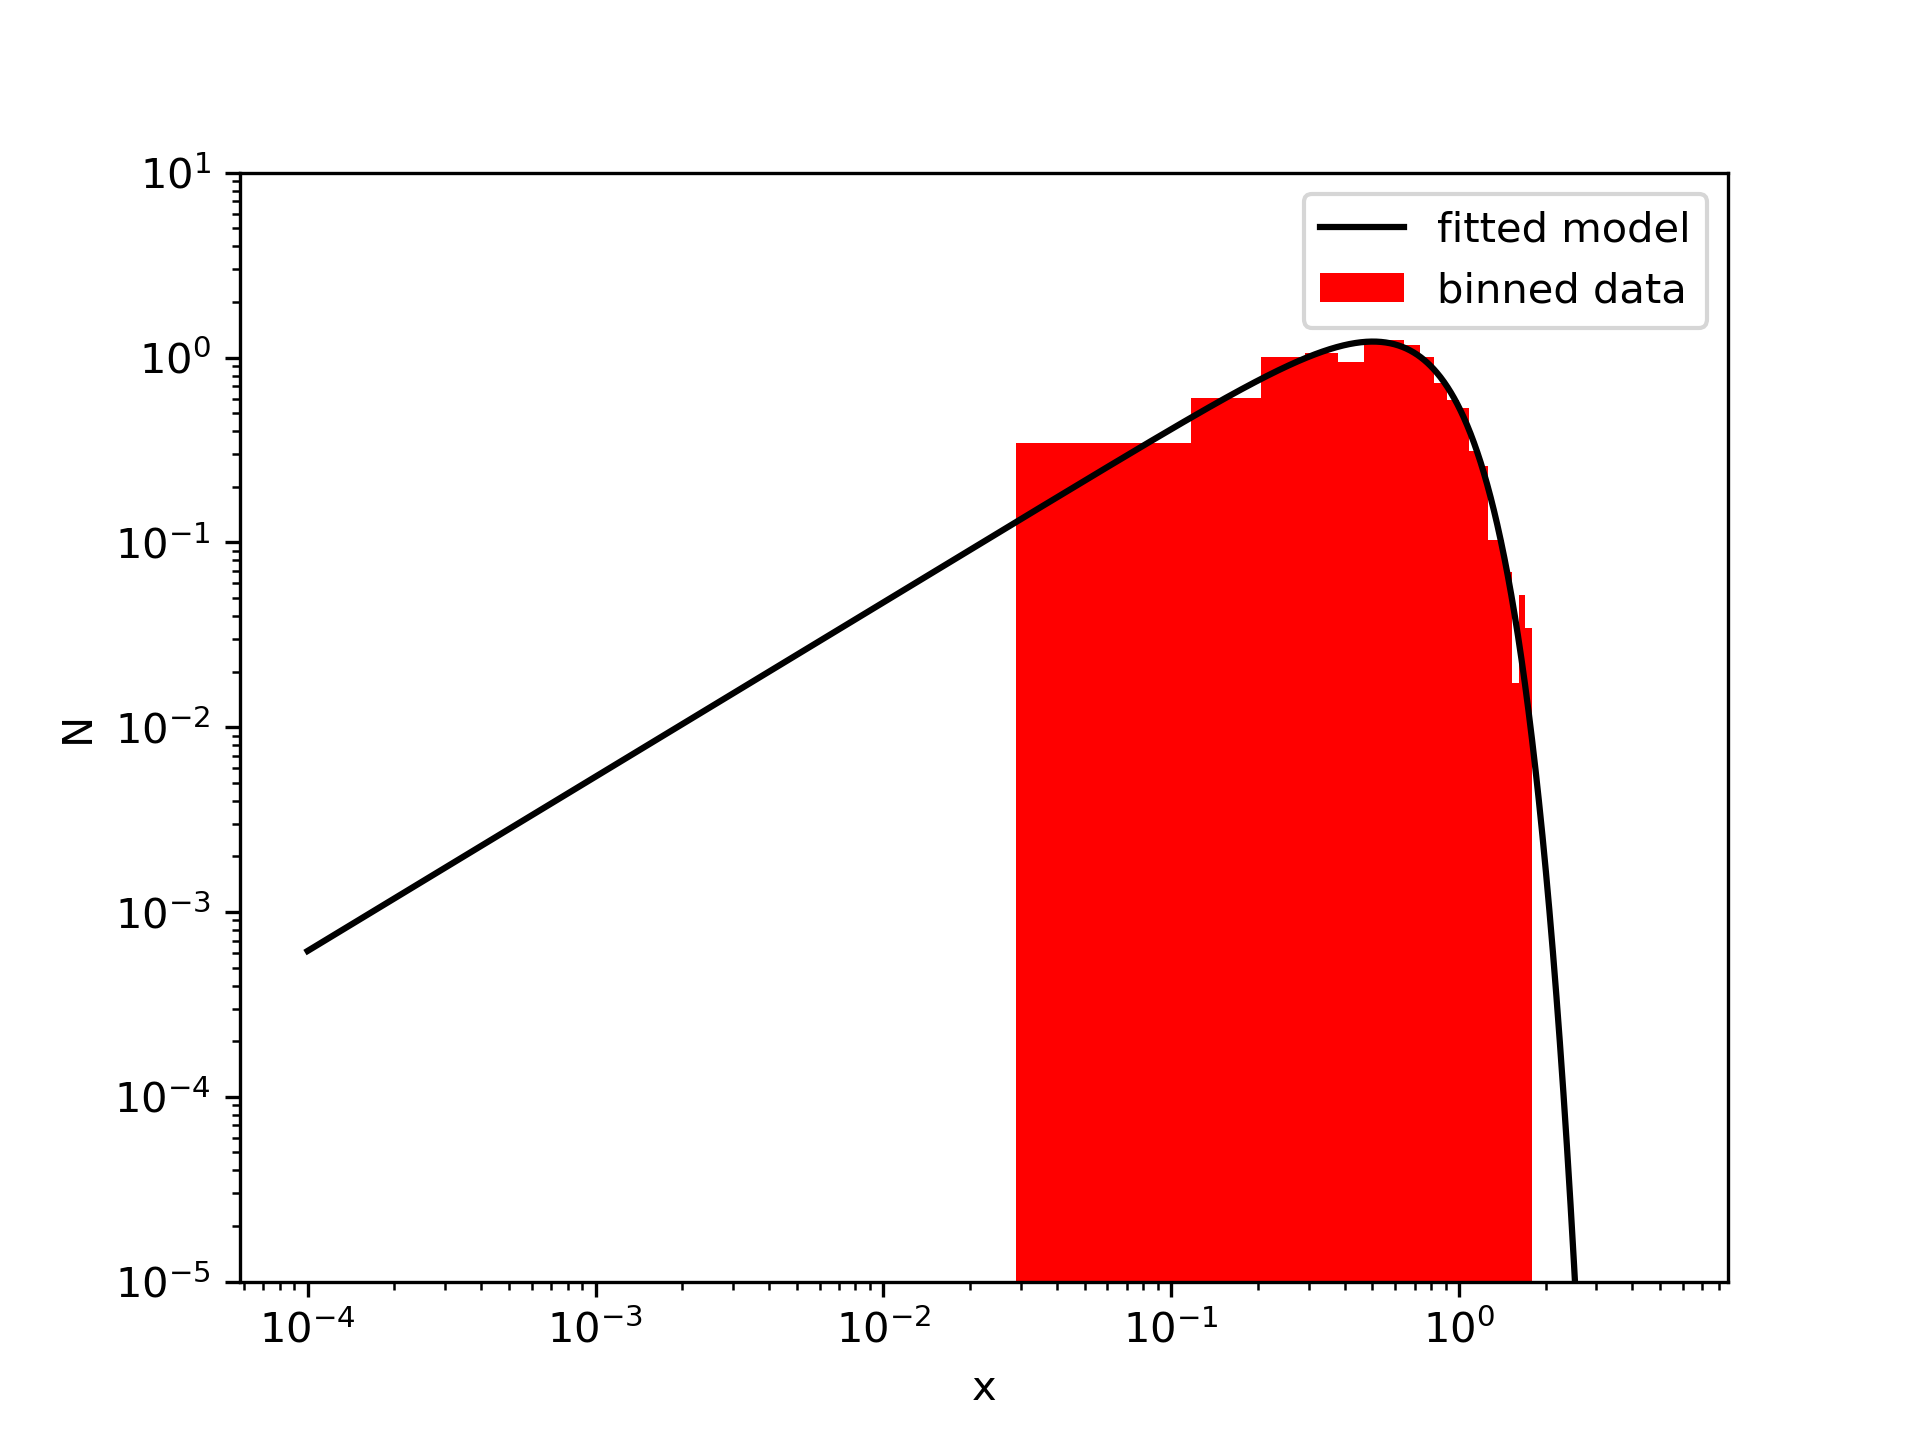
\includegraphics[width=.48\linewidth]{./plots/pois-fit5.png}
  \caption{The binned data with the best-fit model for each dataset. The plot is in logarithmic scale for both the x and the y axis. To fit the model we minimized Poisson log-likelihood. We can see that the model greatly fits our data in all five cases.}
  \label{fig:pois-fit}
\end{figure}

\lstinputlisting{output/likelihood.txt}

\subsection{Statistical tests}
\label{chap:stat}

In this section, we want to test our fitting by using two different statistical tests. The first one is the G-test which computes the G-value using the formula:
\begin{equation}
  G = 2 \sum_{i} O_i \ln(\frac{O_i}{E_i})
\end{equation}
where $O_i,\, E_i$ are the observed and expected number of counts in each bin. After calculating this value we compute the probability by calculating:
\begin{equation}
  P(G,k) = \frac{\gamma(\frac{k}{2},\frac{G}{2})}{\Gamma(\frac{k}{2})}
\end{equation}
where $\gamma$ is the incomplete $\Gamma$ function and $k$ are the degrees of freedom. For our problem, the degrees of freedom can be calculated by subtracting the number of parameters (3) from the number of bins that were used for each dataset. Although during our implementation we calculate this value for each dataset to make the code more generalized, the value of $k$ for all cases is 17 as we have 20 bins for all the datasets. When we have the probability we calculate the Q-value which is equivalent to the more known p-value by using the equation:
\begin{equation}
  \label{eq:Q}
  Q = 1 - P(G,k)
\end{equation}

The second test we want to implement is the Kolmogorov-Smirnov test more known as the K-S test. We now want to calculate the cdf of both our observations and our fitted model. We then calculate the maximum difference between the two of them which is denoted as $D$ and used to calculate z using the formula:
\begin{equation}
  z = (\sqrt{N}+0.12+\frac{0.11}{\sqrt{N}}) D
\end{equation}
where $N$ is the number of bins that were used to bin our observations. We then use $z$ to calculate the K-S probability. To do this in the numerically optimal way we use one of the two formulas depending on the value of $z$ 
\begin{equation}
  P_{KS}(z) = \frac{\sqrt{2 \pi}}{z}[(e^{-\pi^2/(8z^2)})+(e^{-\pi^2/(8z^2)})^9+(e^{-\pi^2/(8z^2)})^25]\:\:\:\: if \:\: z<1.18
\end{equation}

\begin{equation}
  P_{KS}(z) = 1-2[(e^{-2z^2})-(e^{-2z^2})^4+(e^{-2z^2})^9] \:\:\:\:\:\:\:\:\:\:\:\:\:\:\:\:\:\:\:\:\:\:\:\:\:\:\:\:\:\:\:\:\: if \:\: z \ge 1.18
\end{equation}

We then calculate the Q-value as we did in the G-test by using \Cref{eq:Q}

In our script, we implement the ``romberg'' function that was already used in our previous assignment to get better results when integrating. We then define our ``G\_test'' function that first calculates the G-value, then the degrees of freedom for our problem (number of bins - 3). Then computes the probability by calling the incomplete $\gamma$ function from the ``scipy'' library. The ``gammainc'' routine already normalizes by diving with $\Gamma(a)=\Gamma(k/2)$, where $a$ is the first term in the ``gammainc'' input. We, therefore, do not have to make this division in our code. 

The function ``ks\_test'' implements the K-S test as it was described before. It calculates the cumulative counts for our data and model and then divides it by the maximum value (last value) to get the cdf. The function then finds the value of the maximum distance between the two (also returns the position for some plots) and then calculates the z value and finally the K-S probability. 

\lstinputlisting{stat_test.py}

In the main part of our script, we compute the test values. This time we will work with the actual number of counts instead of the pdf which was used when we were fitting our models. We, therefore, bin our data with no normalization and define our average number of galaxies for each dataset to be equal to the actual number of galaxies in each dataset. We then get the x position of the bin centers for each data set. After that, we calculate the model in this position by integrating over each bin. This job is done for all the datasets and for both the $\chi^2$ and Poisson minimization. Finally, we call the test functions and output the results. We also create some plots for better visualization.

\lstinputlisting{output/stat_test.txt}

The output of our script is very interesting as the Q-values of the G-test suggest that our fitting is not that great for almost all of the cases. We know that this is not the case and the Q-values from the K-S test confirm that we indeed have a great fit for all our models. The problem with the values of the G-test probably has to do with errors in the integration as experimentation using our script has shown that is indeed very sensitive to different calculations of the normalizing parameter $A$. This is the main reason we decided to use the ``romberg'' function to integrate instead of the more simple ``trapezoid'' function. 

It is however still evident that the Poisson log-likelihood minimization worked better in all the cases except for m14 where the G-values were very similar and slightly better for the $\chi^2$ minimization. We can therefore conclude that the minimization of the negative Poisson log-likelihood worked much better and fitted our observations with more detail. 

We can also see how great the match between the observed and model cdf is in \Cref{fig:ks_chi,fig:ks_pois}. The maximum difference between the two for each case is shown with a red vertical line that is very easy to miss because the match is almost perfect which makes the line very small.  

%references
\bibliographystyle{apacite}
\bibliography{TeX/references_3}

\newpage

\appendix
\section{Extra Plots}
\label{chap:append}

\begin{figure}[H]
  \centering
  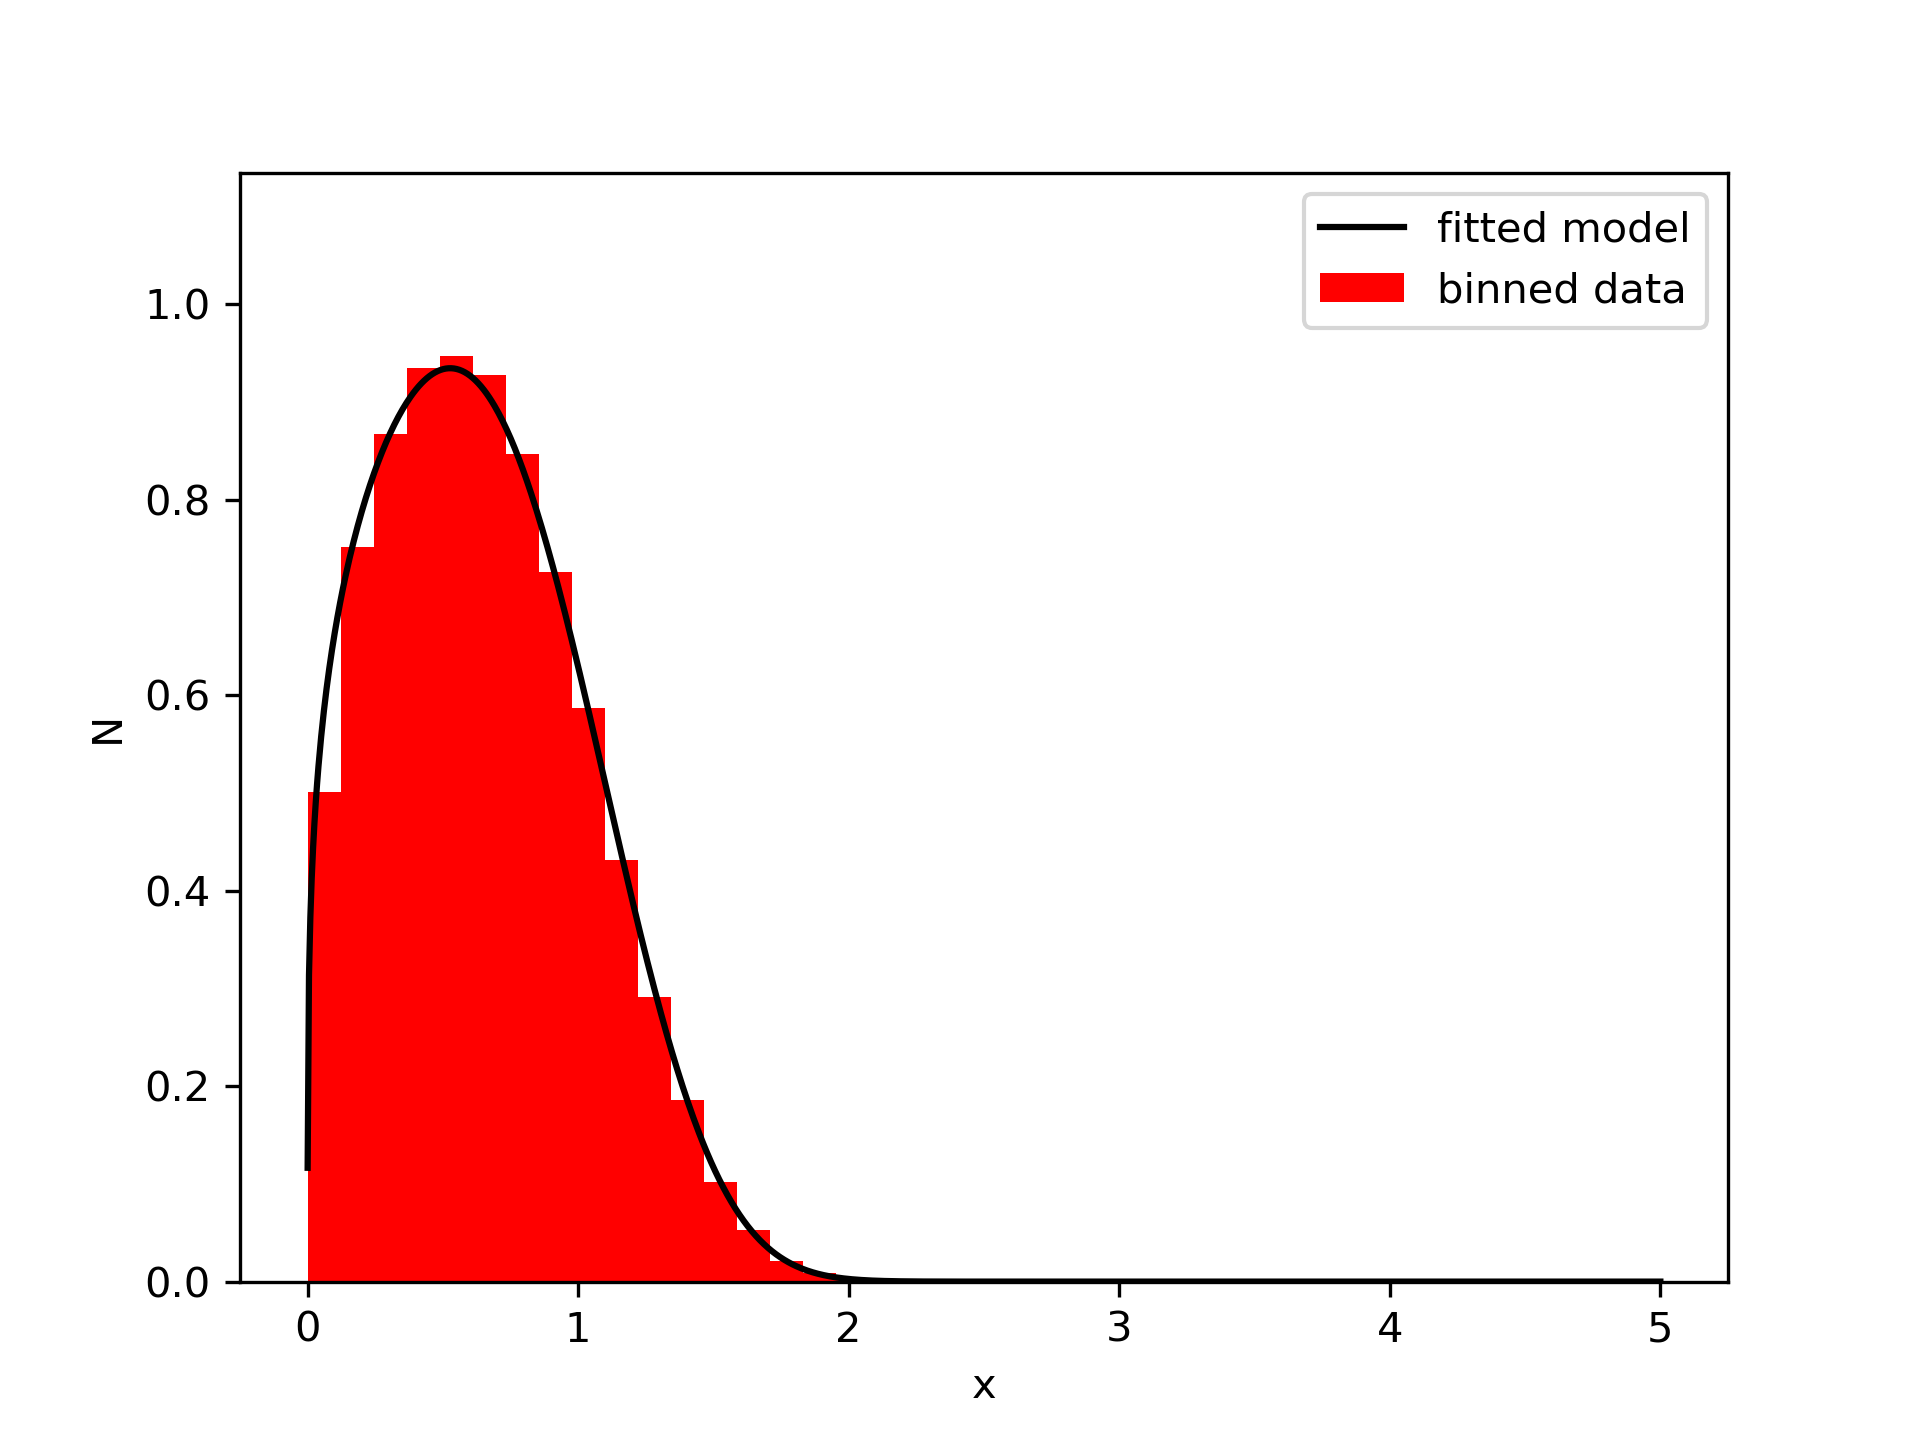
\includegraphics[width=.48\linewidth]{./plots/chi-fit-app1.png}
  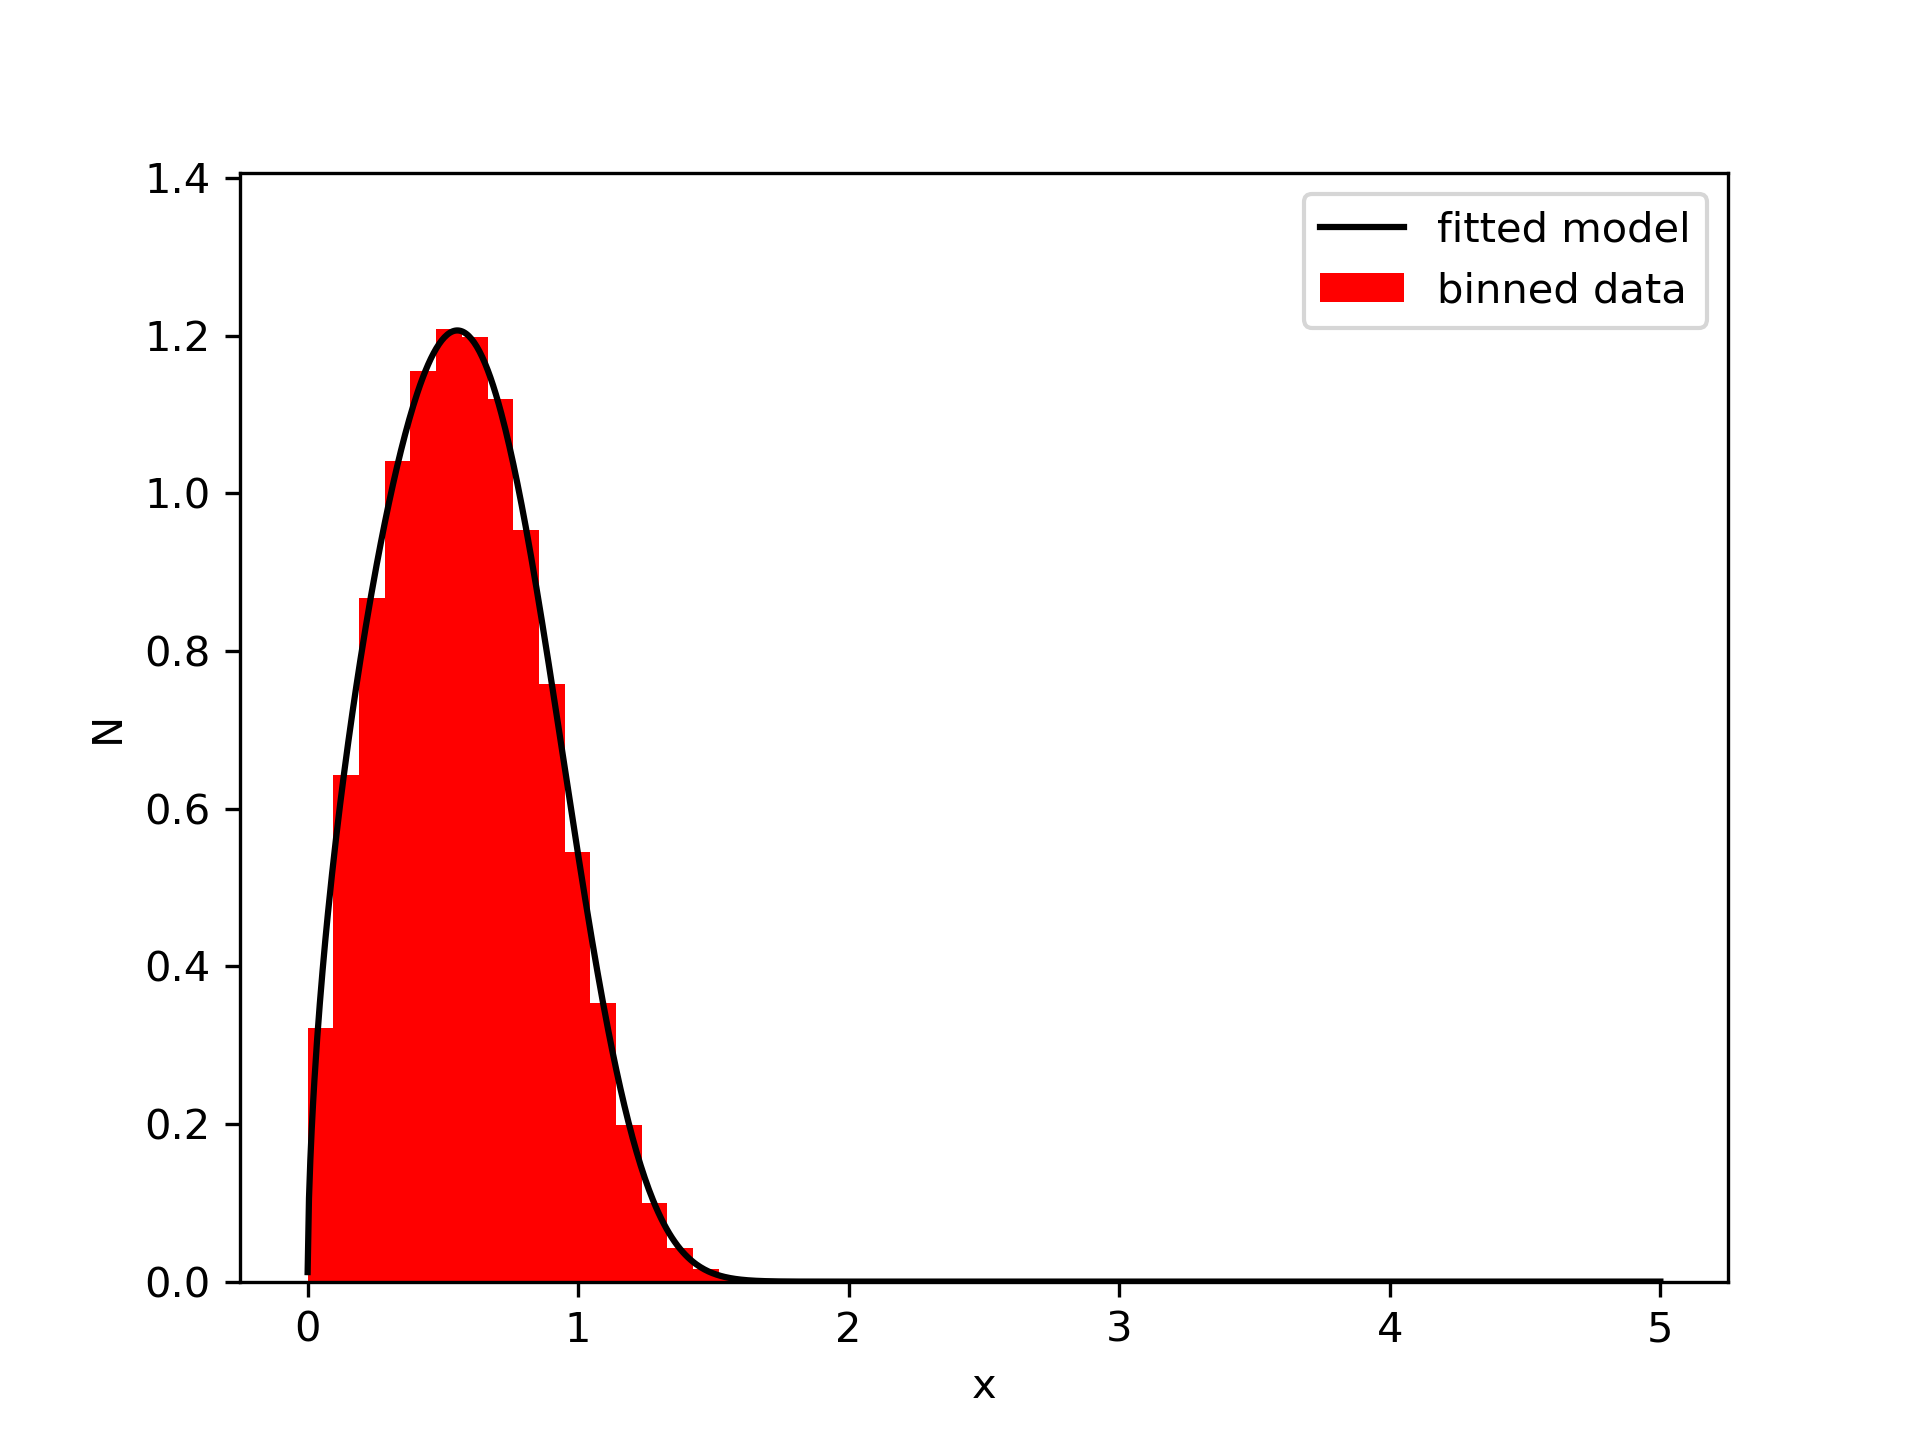
\includegraphics[width=.48\linewidth]{./plots/chi-fit-app2.png}
  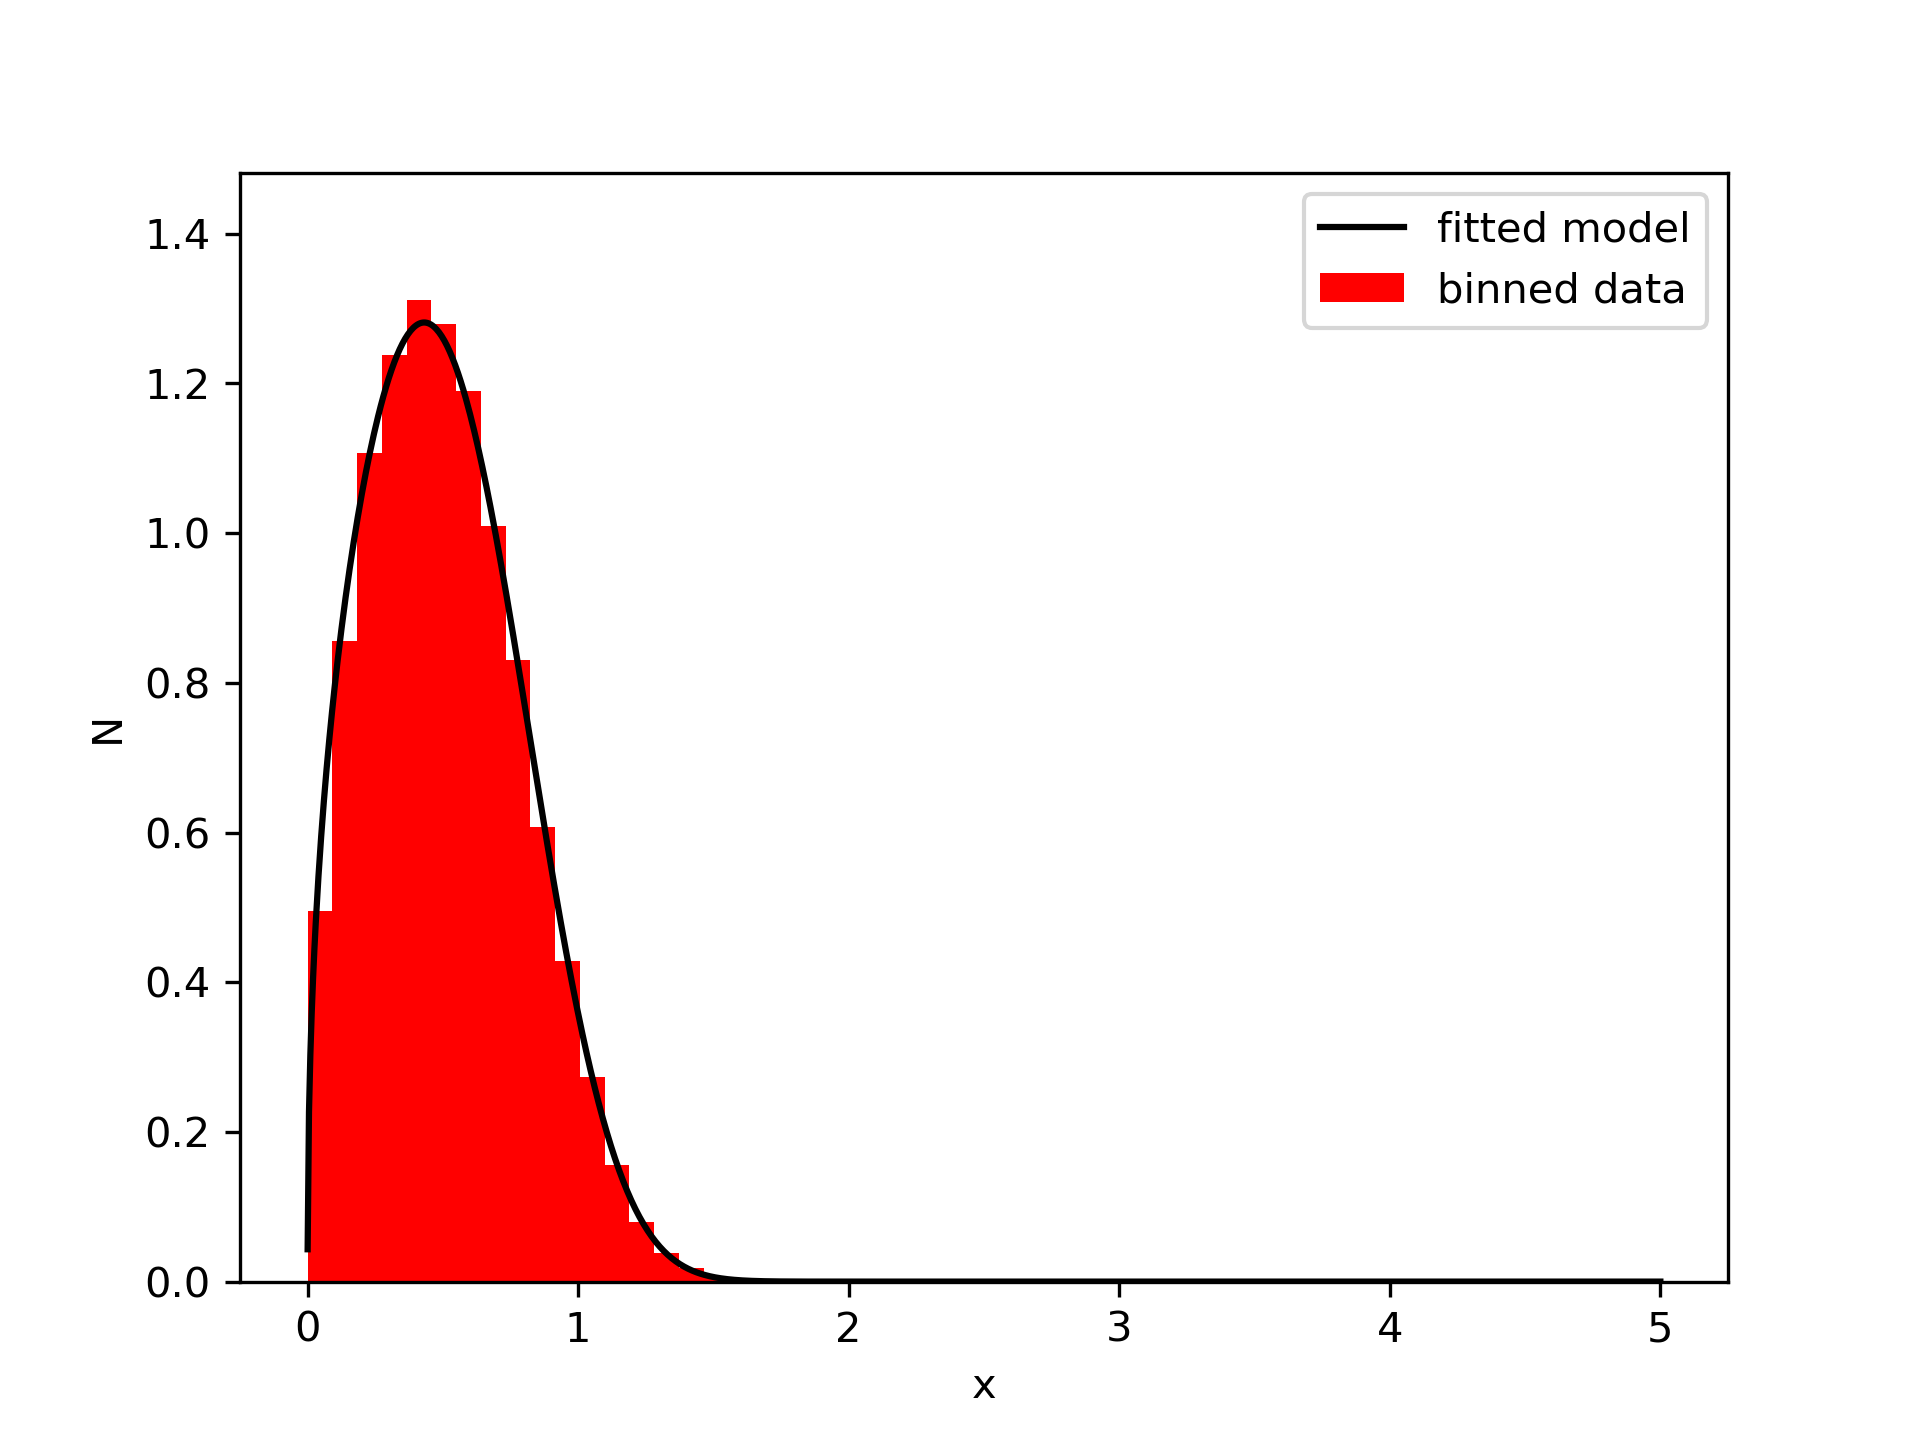
\includegraphics[width=.48\linewidth]{./plots/chi-fit-app3.png}
  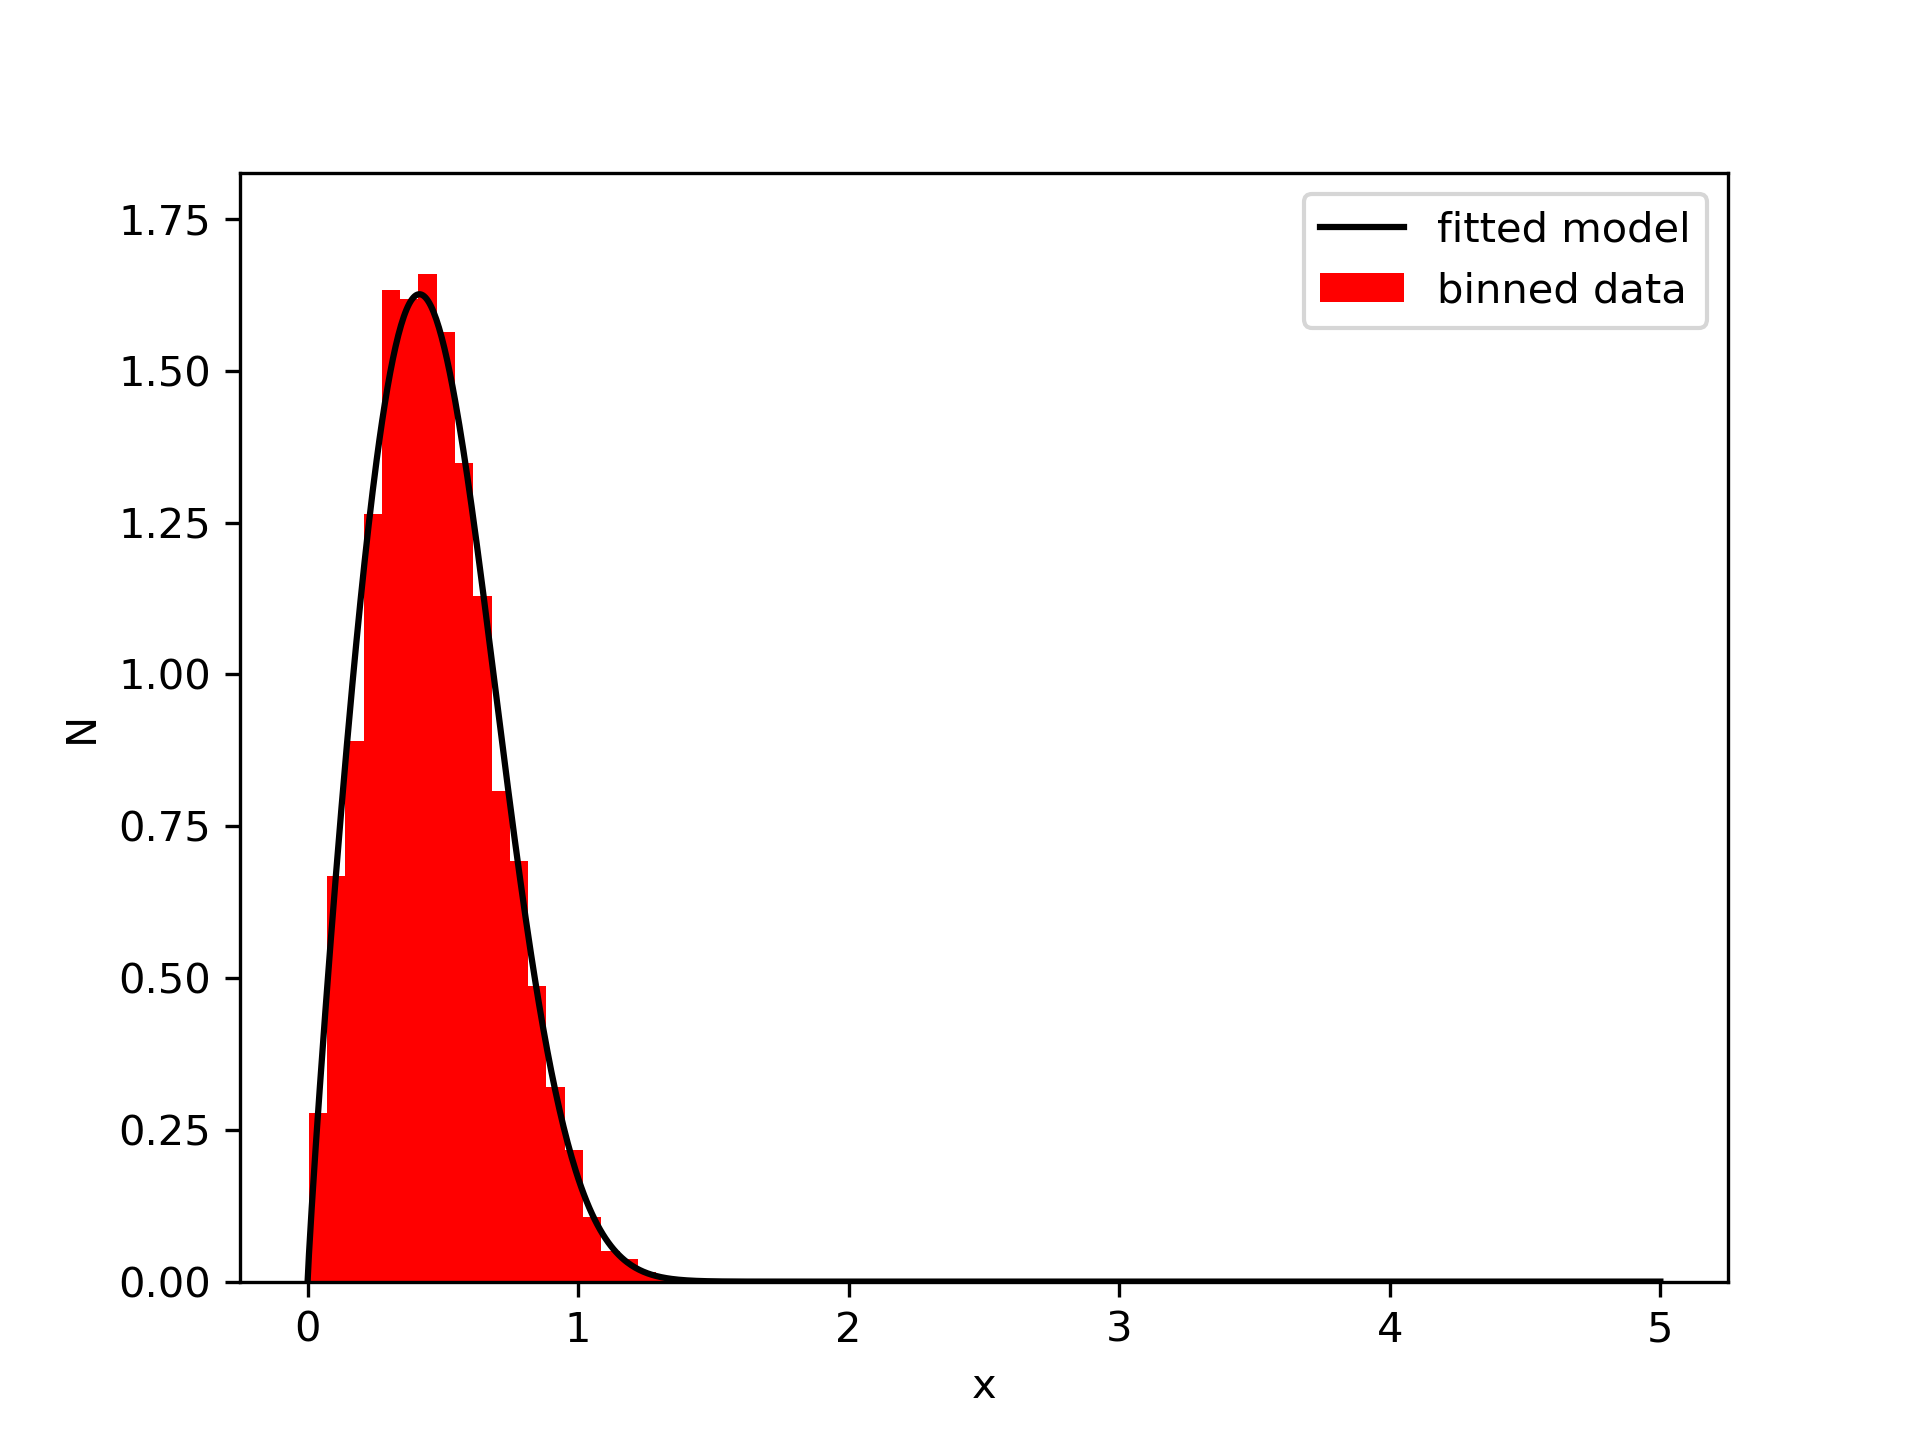
\includegraphics[width=.48\linewidth]{./plots/chi-fit-app4.png}
  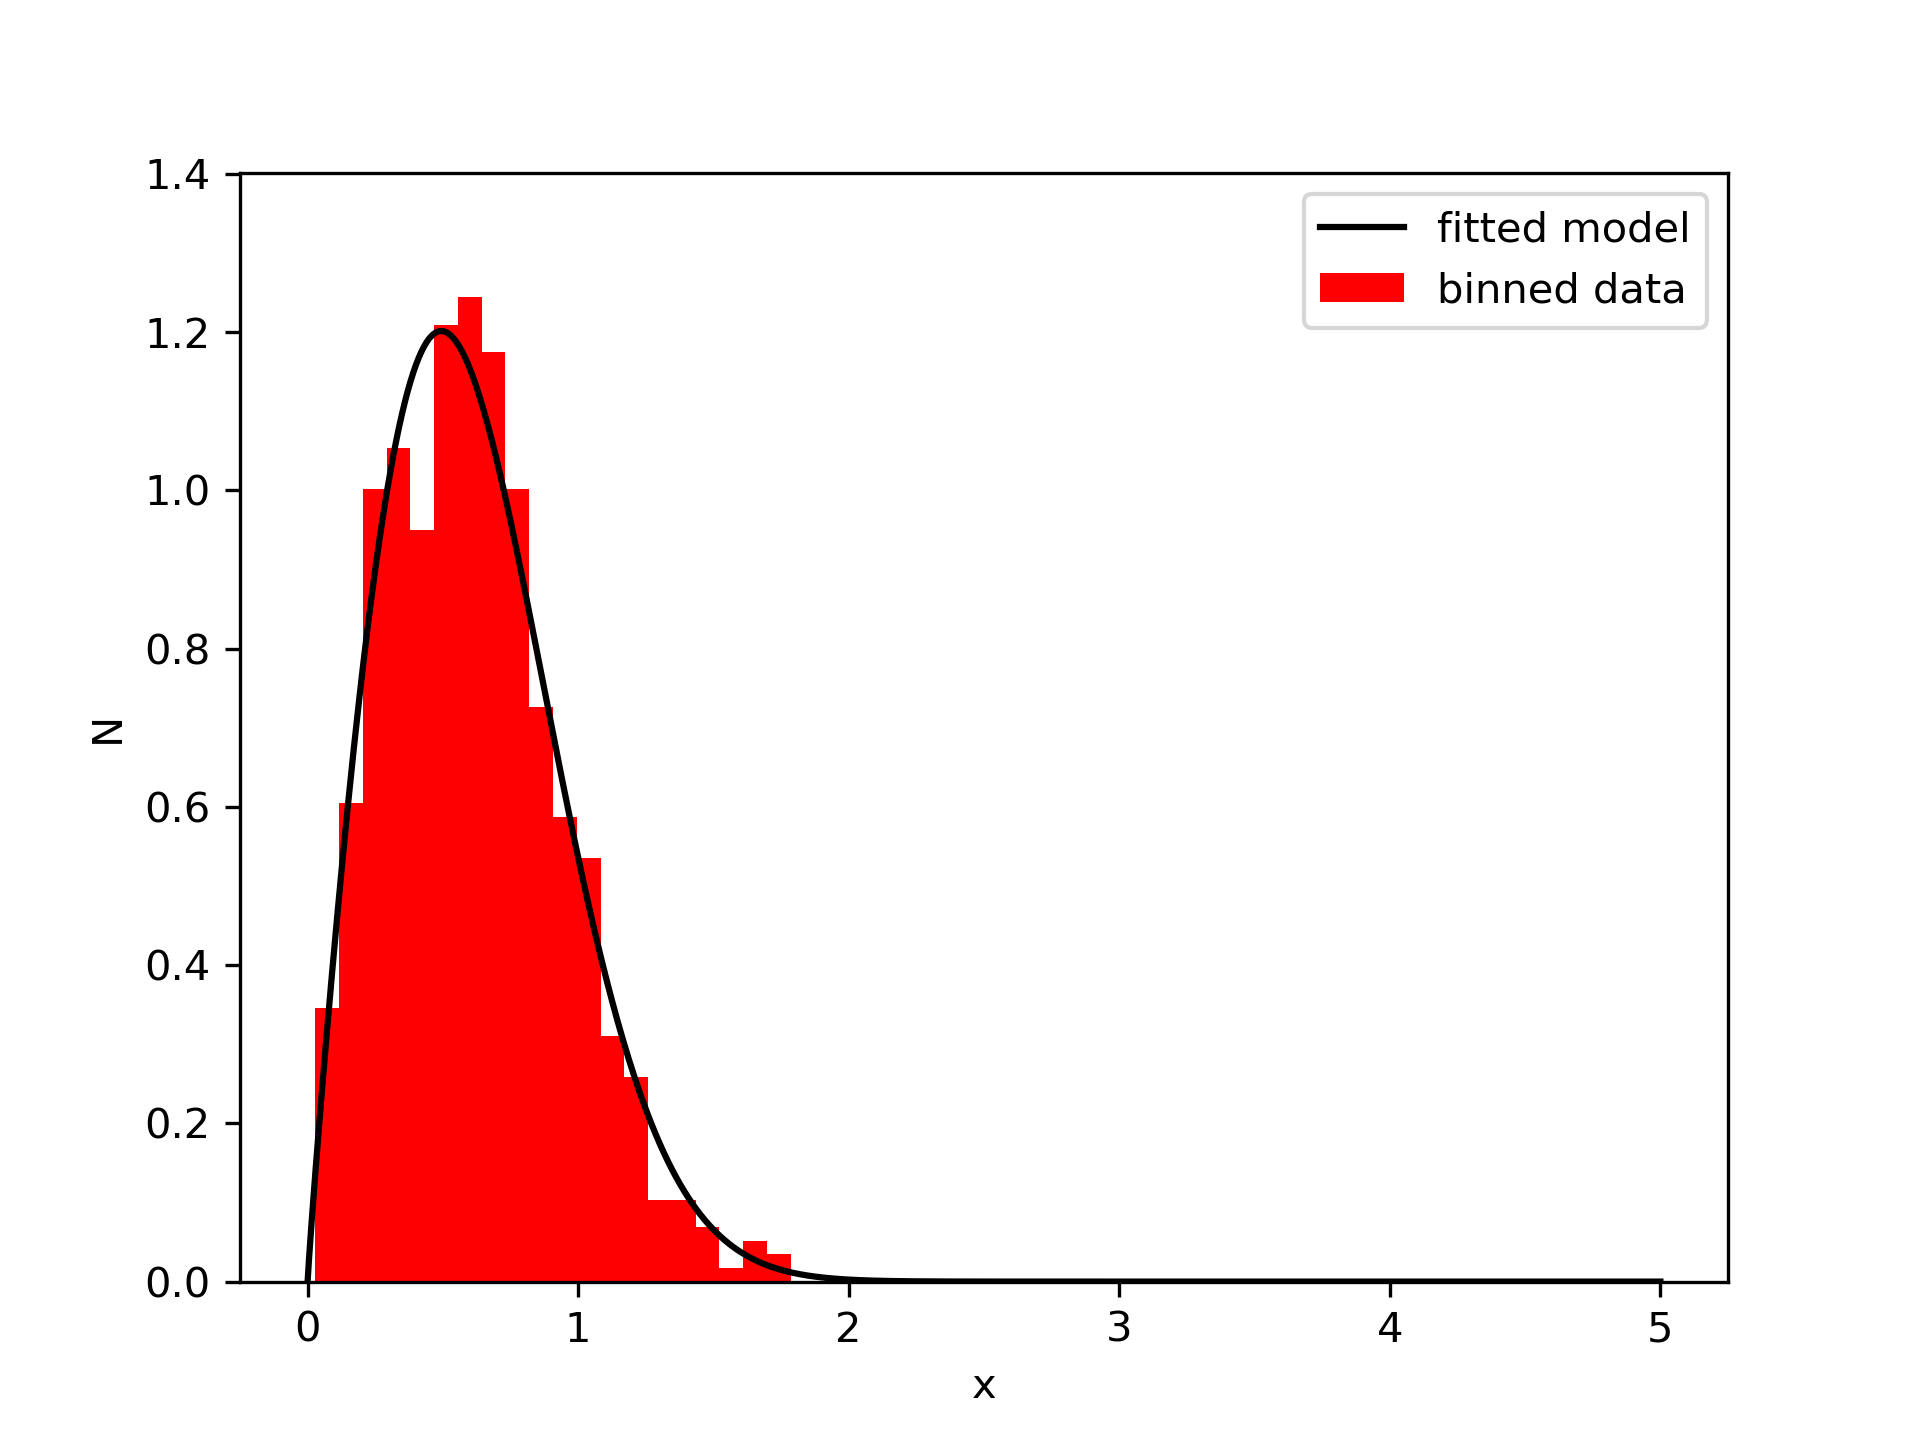
\includegraphics[width=.48\linewidth]{./plots/chi-fit-app5.png}
  \caption{The binned data with the best-fit model for each dataset in real space. To fit the model we minimized $\chi^2$ function. We can see that the model greatly fits our data in all five cases. }
  \label{fig:chi-fit-app}
\end{figure}

\begin{figure}[H]
  \centering
  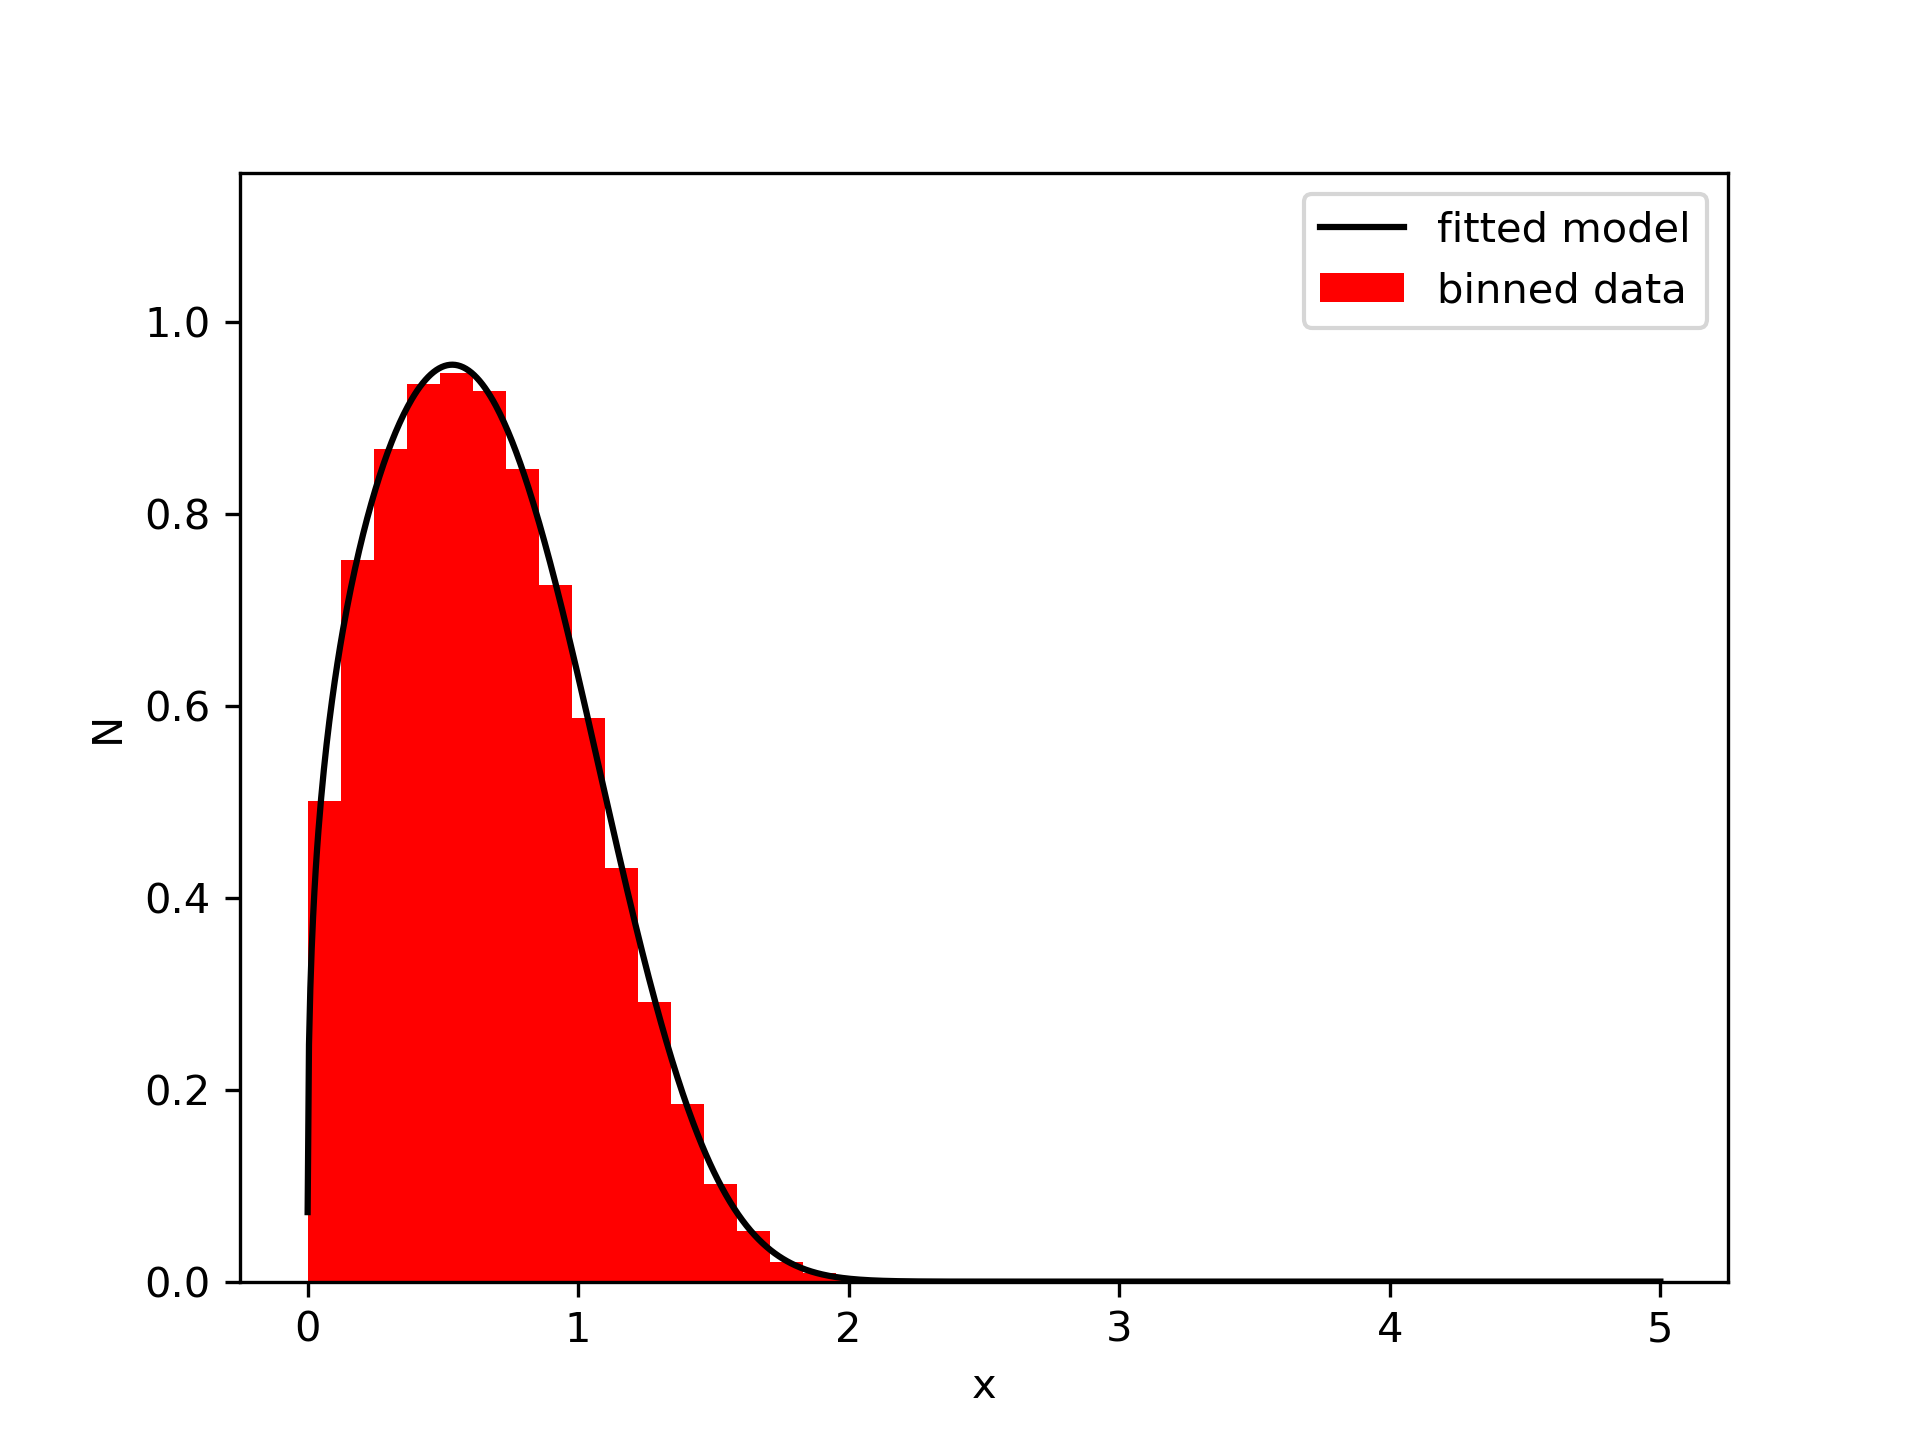
\includegraphics[width=.48\linewidth]{./plots/pois-fit-app1.png}
  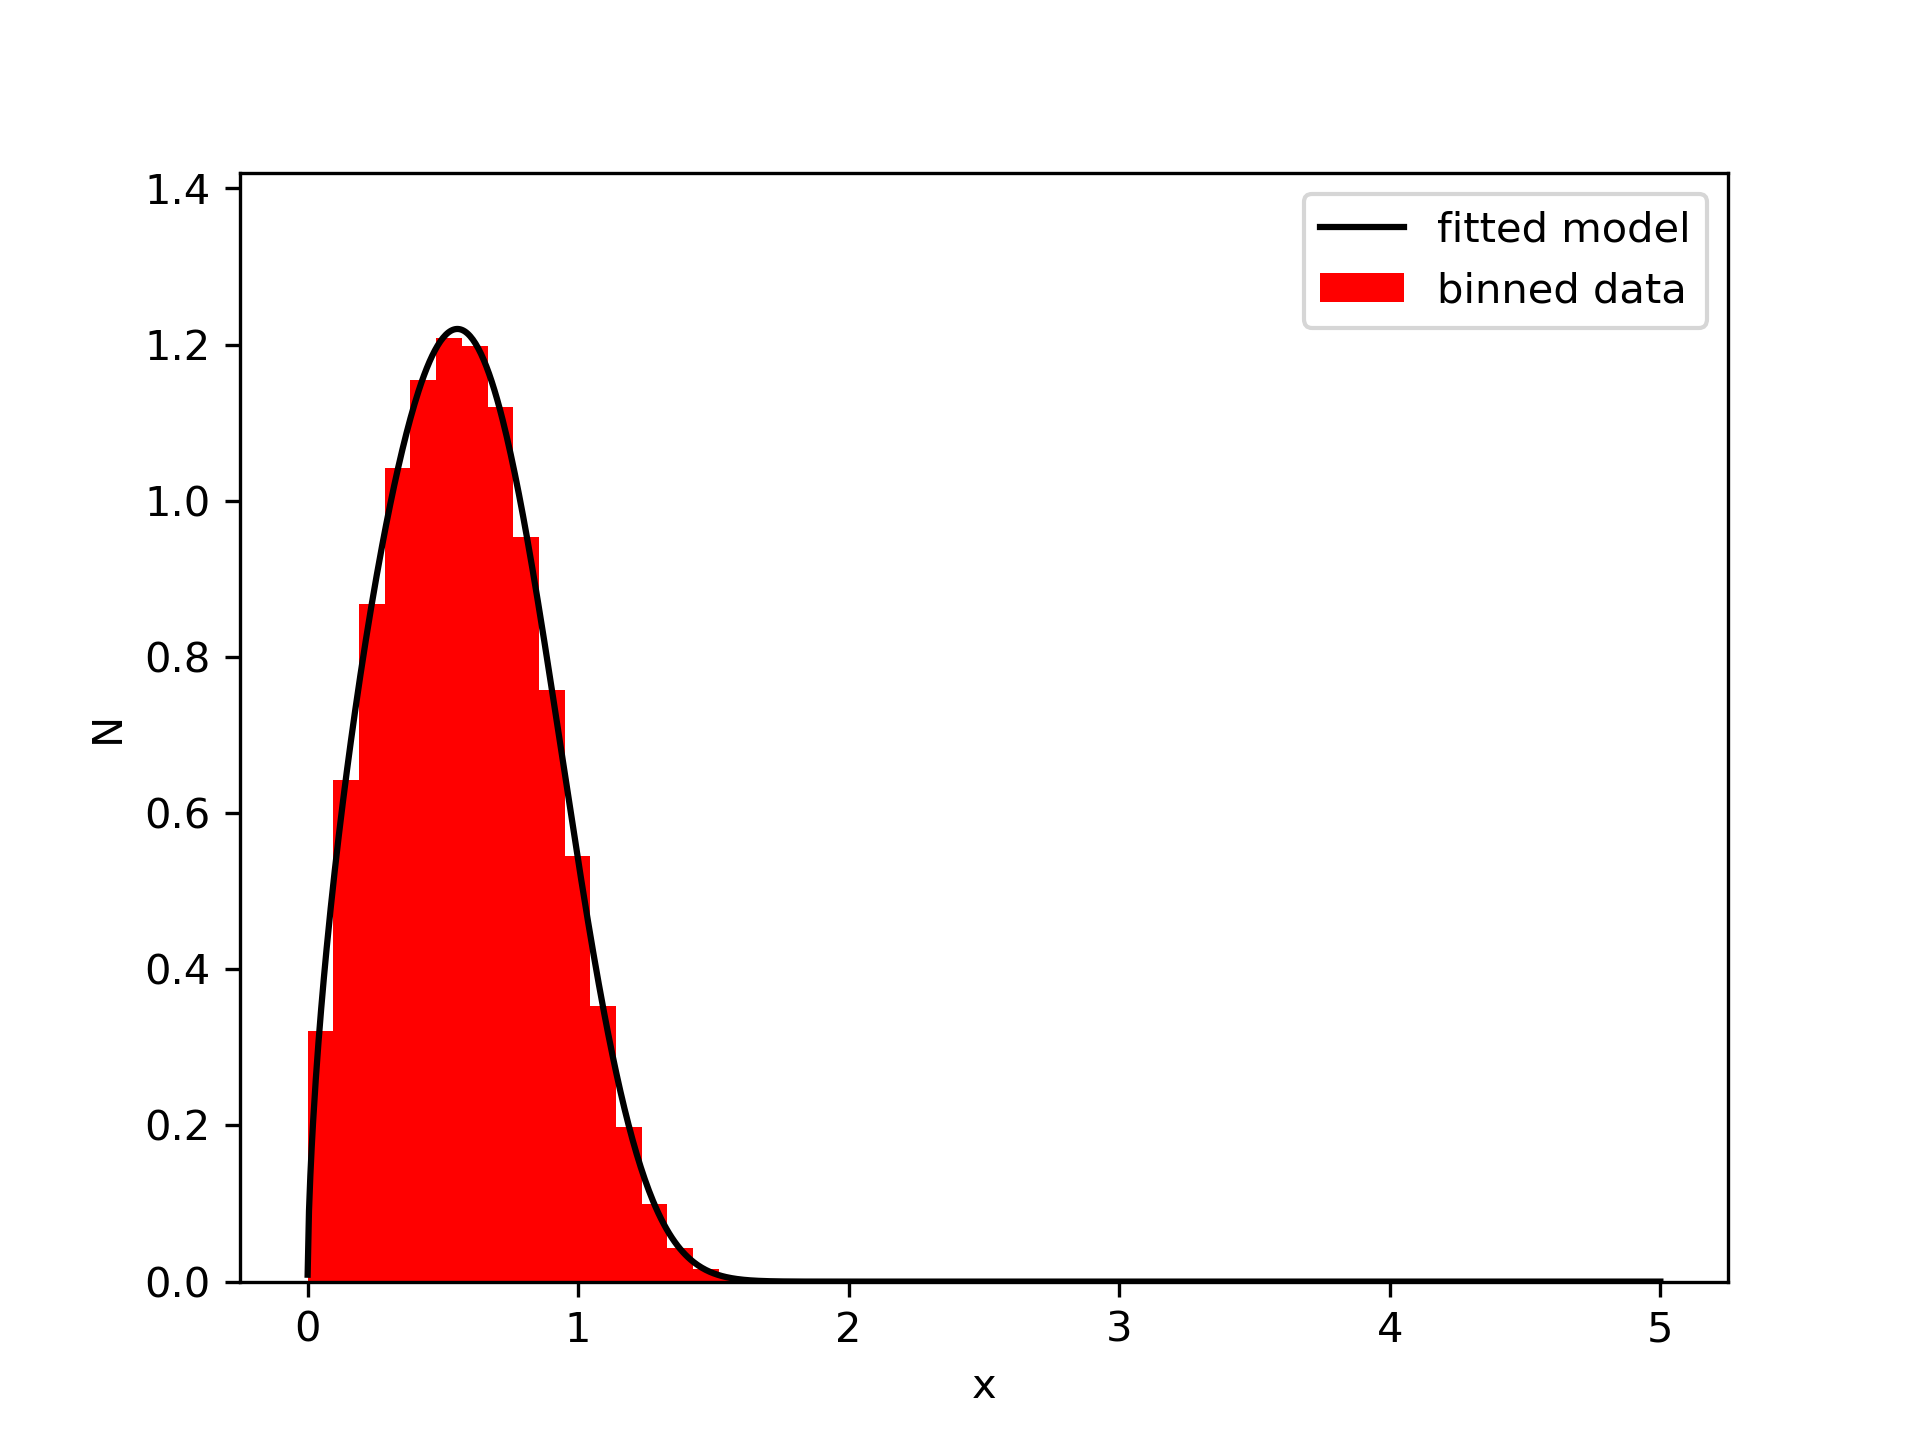
\includegraphics[width=.48\linewidth]{./plots/pois-fit-app2.png}
  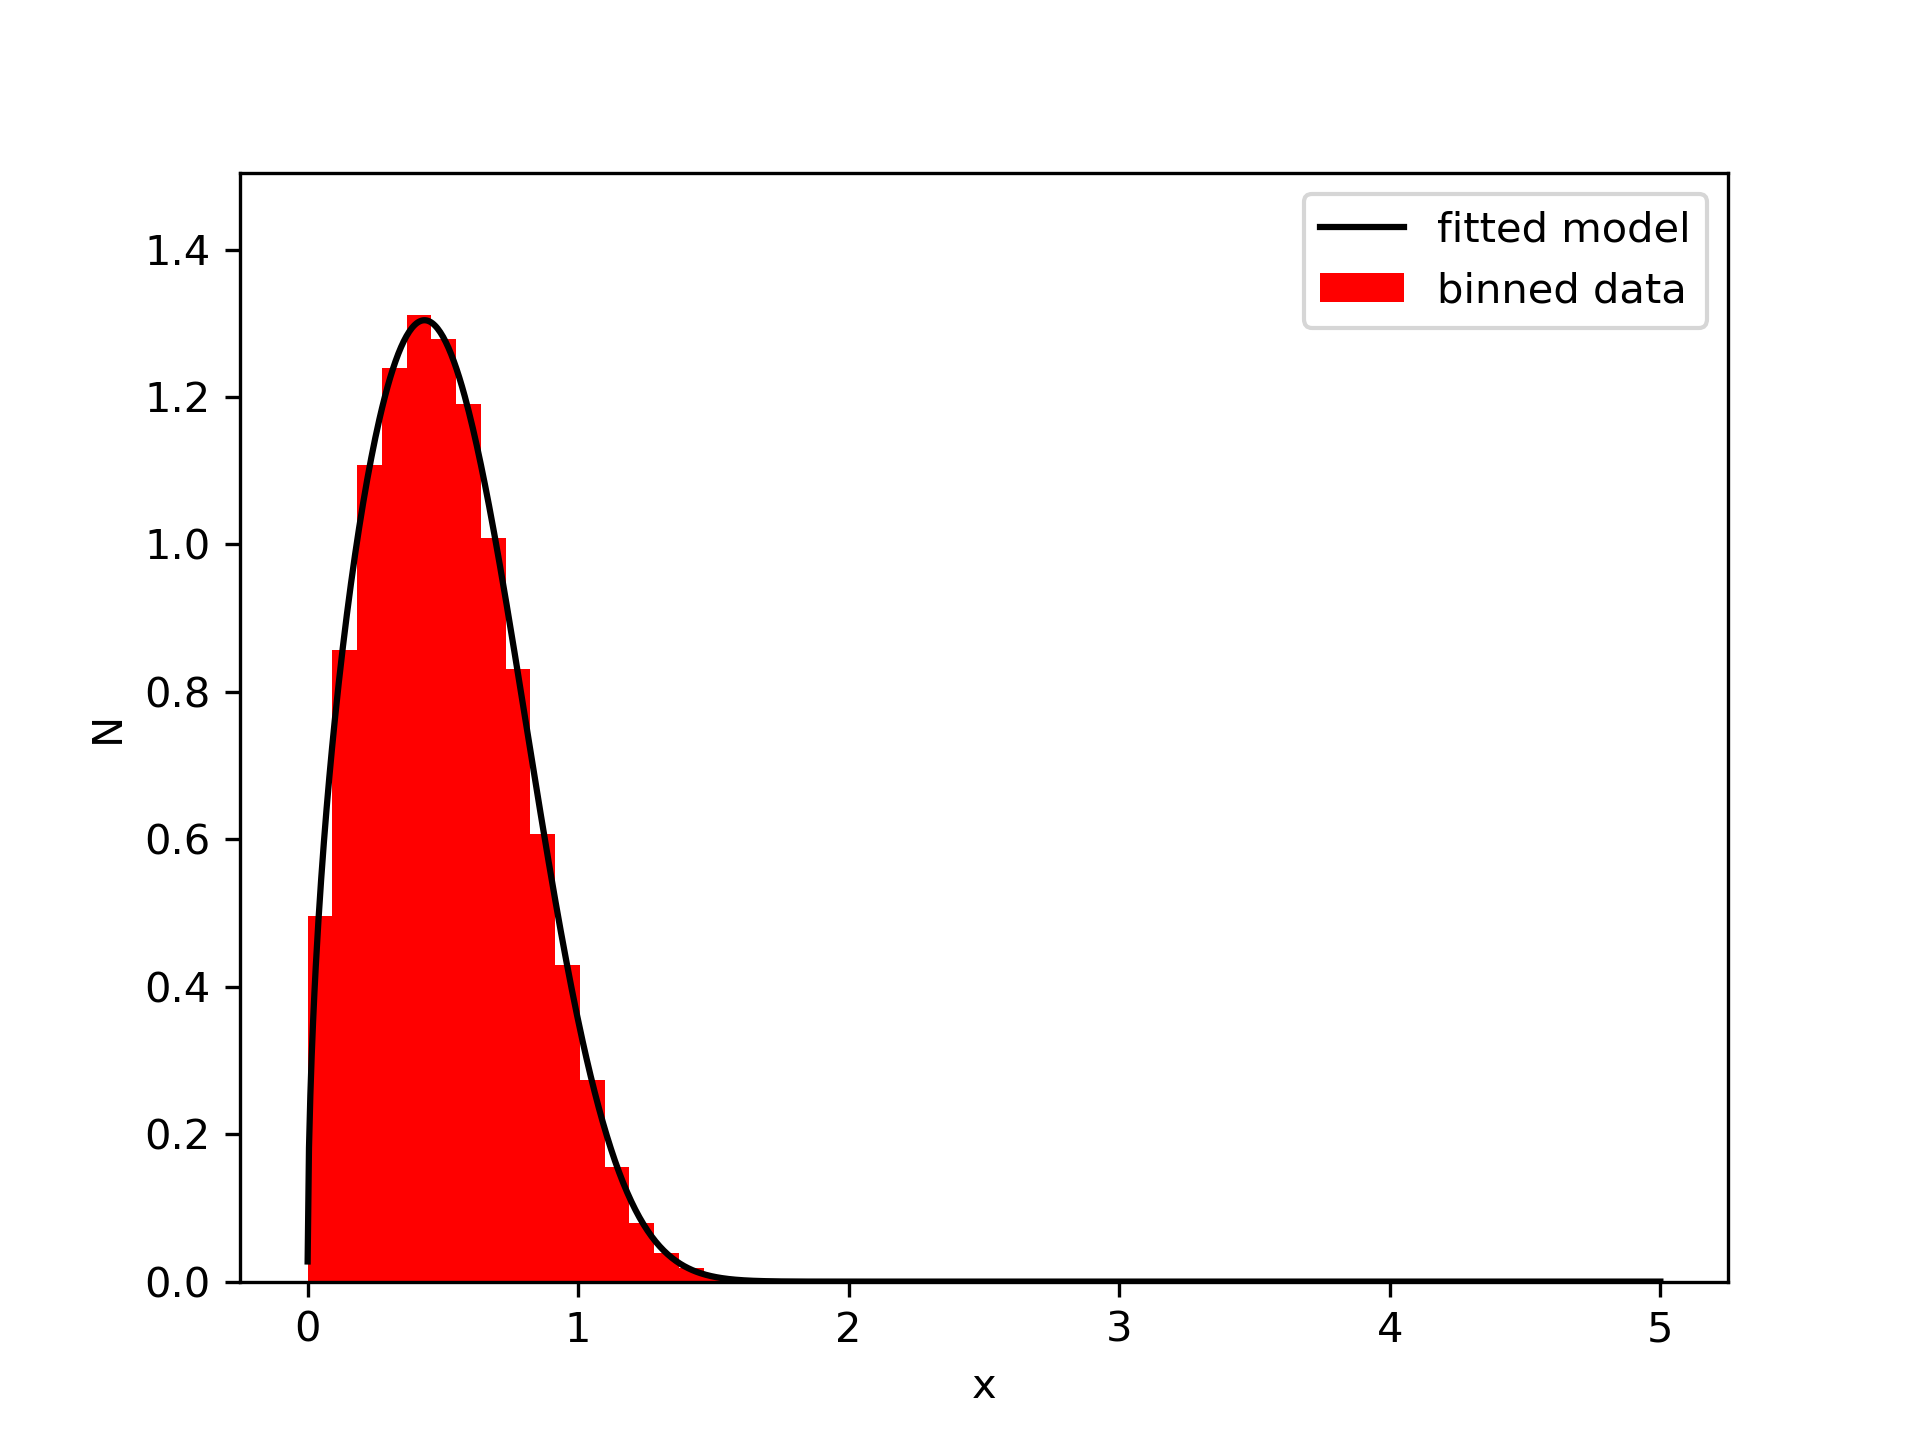
\includegraphics[width=.48\linewidth]{./plots/pois-fit-app3.png}
  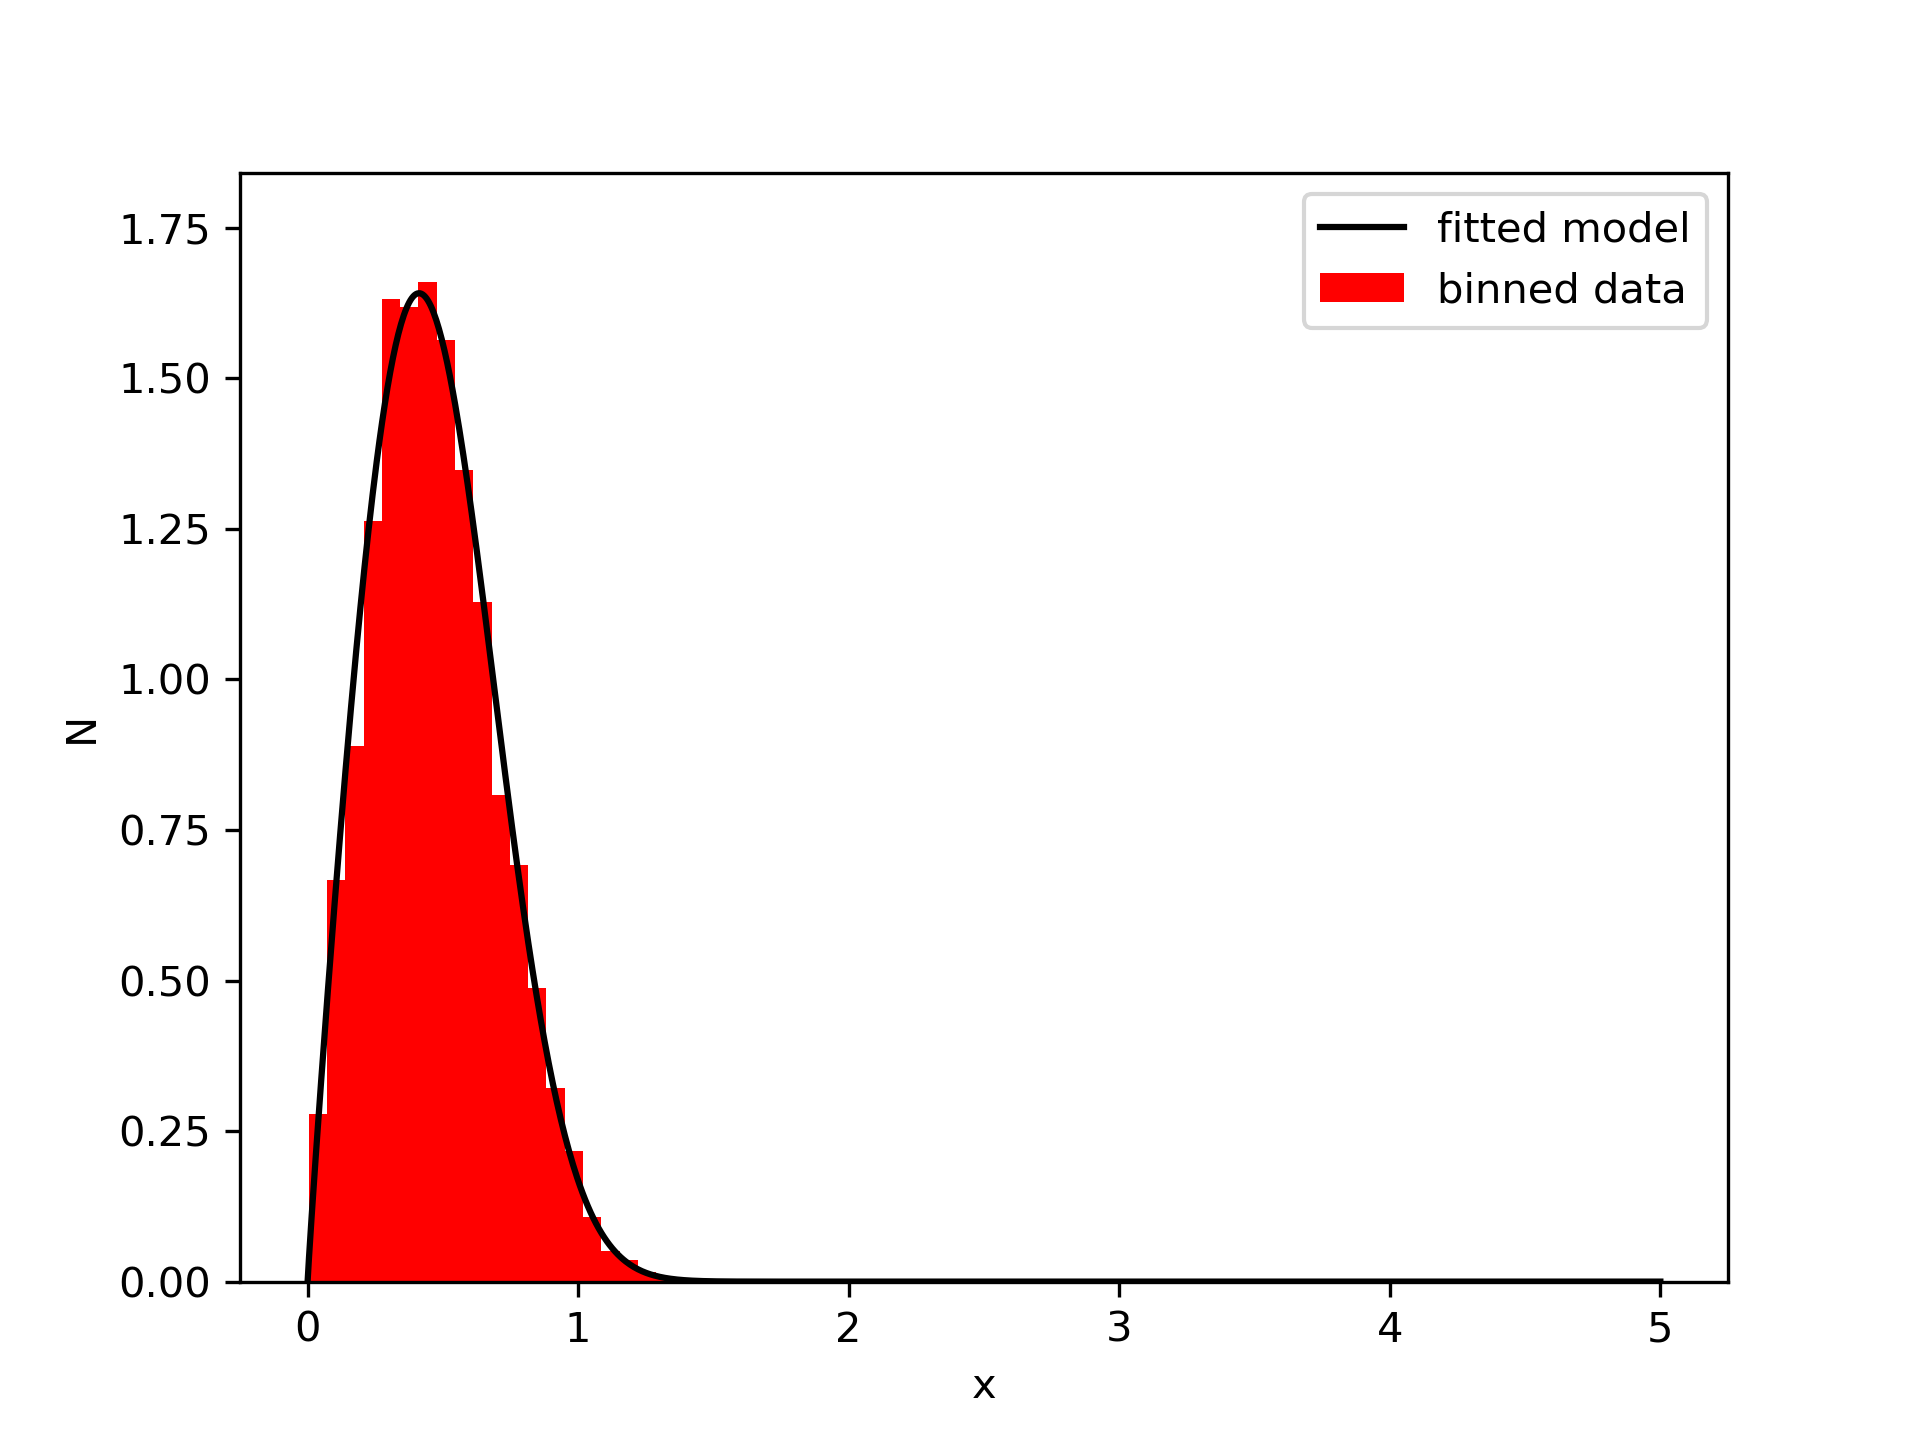
\includegraphics[width=.48\linewidth]{./plots/pois-fit-app4.png}
  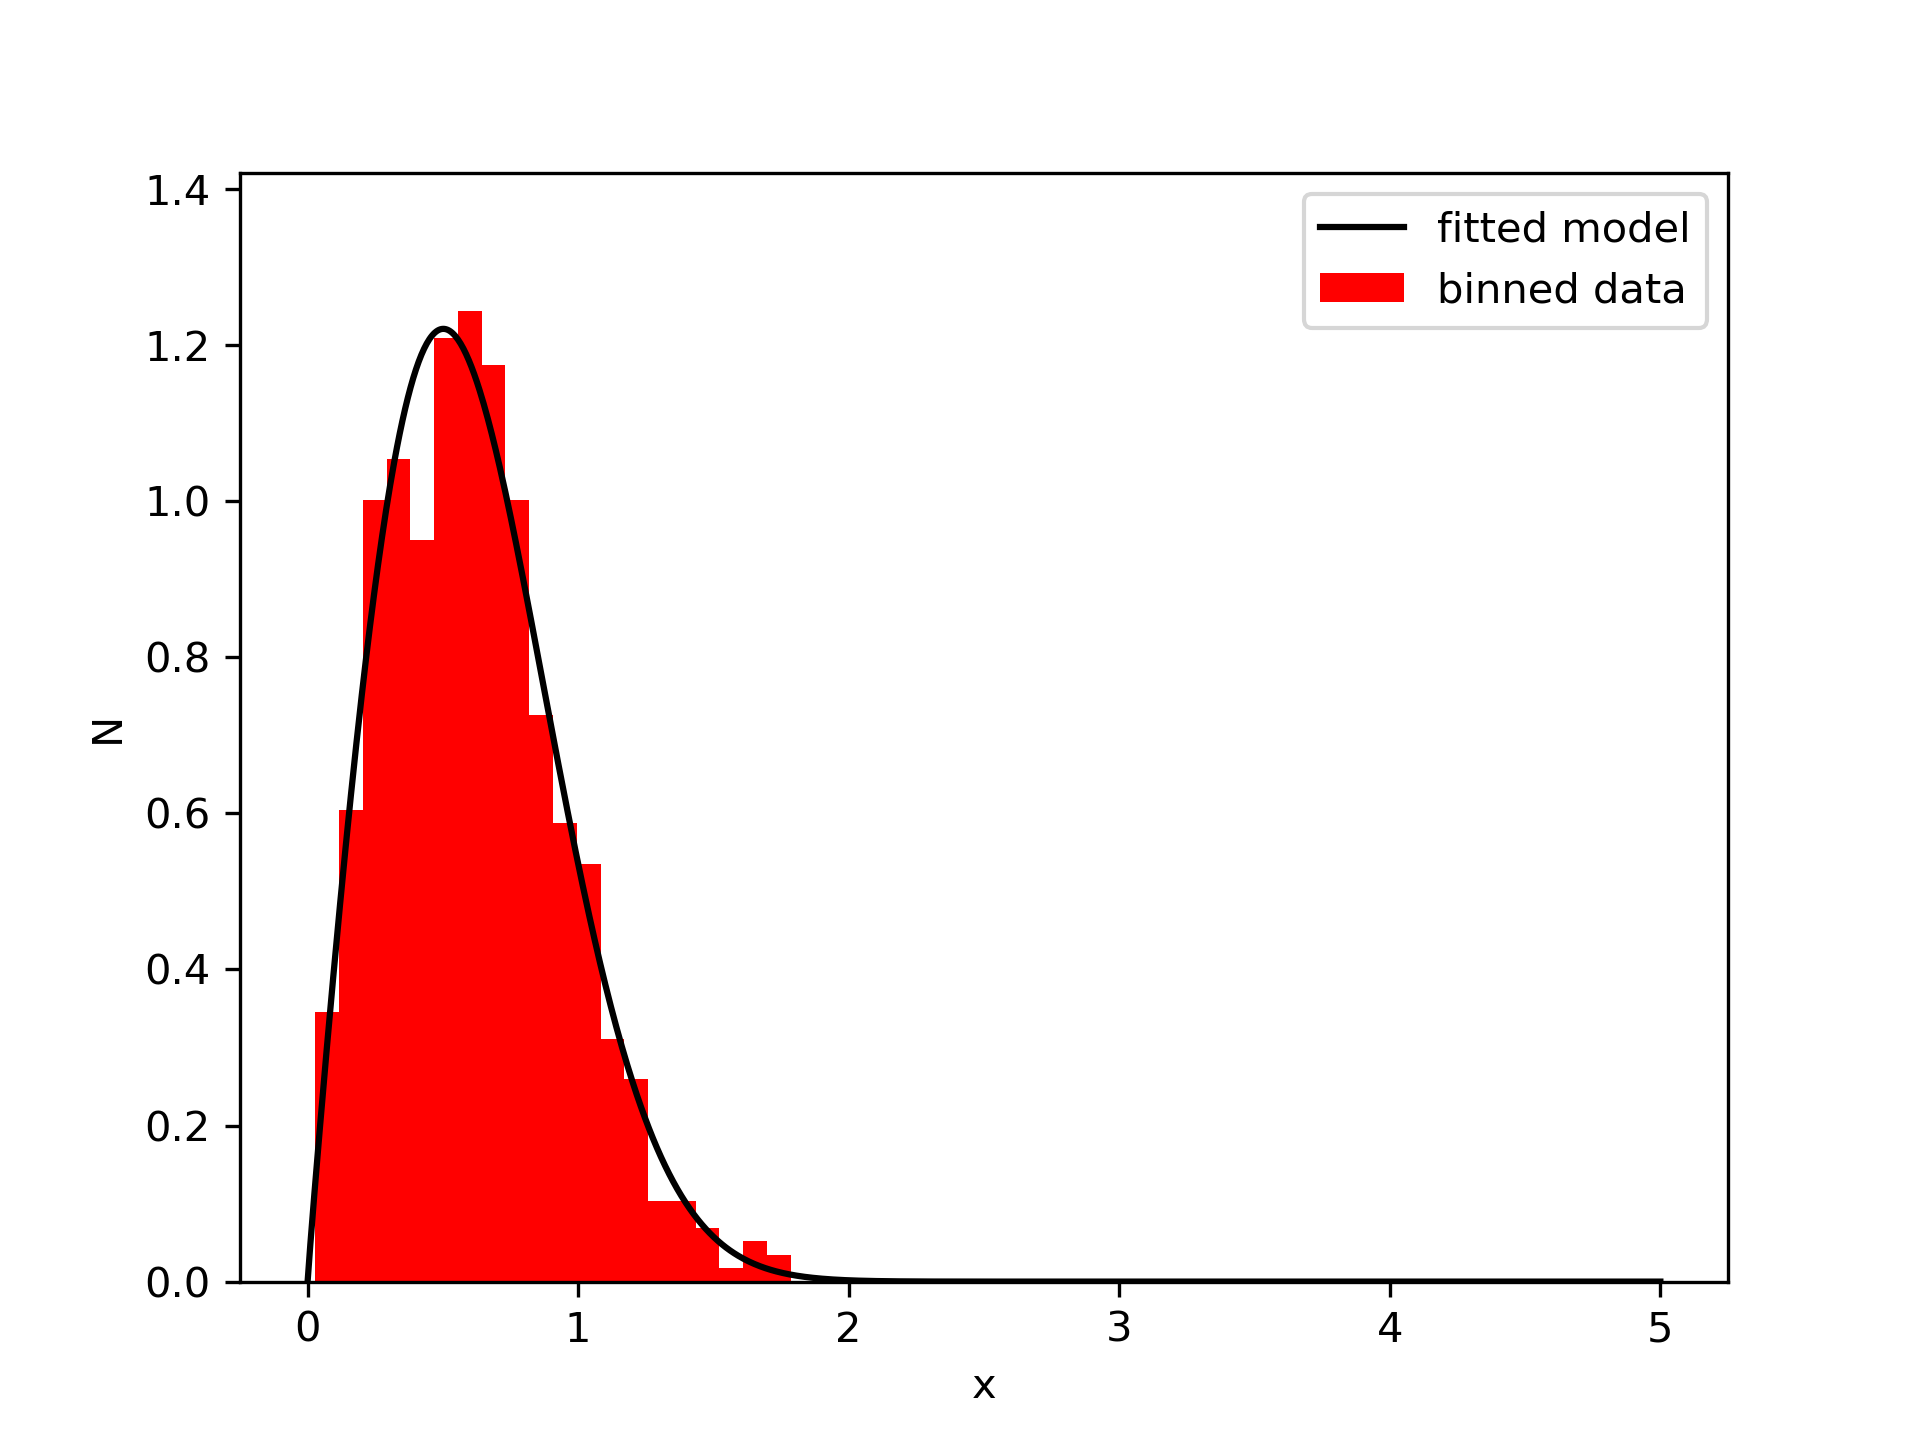
\includegraphics[width=.48\linewidth]{./plots/pois-fit-app5.png}
  \caption{The binned data with the best-fit model for each dataset in real space. To fit the model we minimized Poisson log-likelihood. We can see that the model greatly fits our data in all five cases.}
  \label{fig:pois-fit-app}
\end{figure}

\begin{figure}[H]
  \centering
  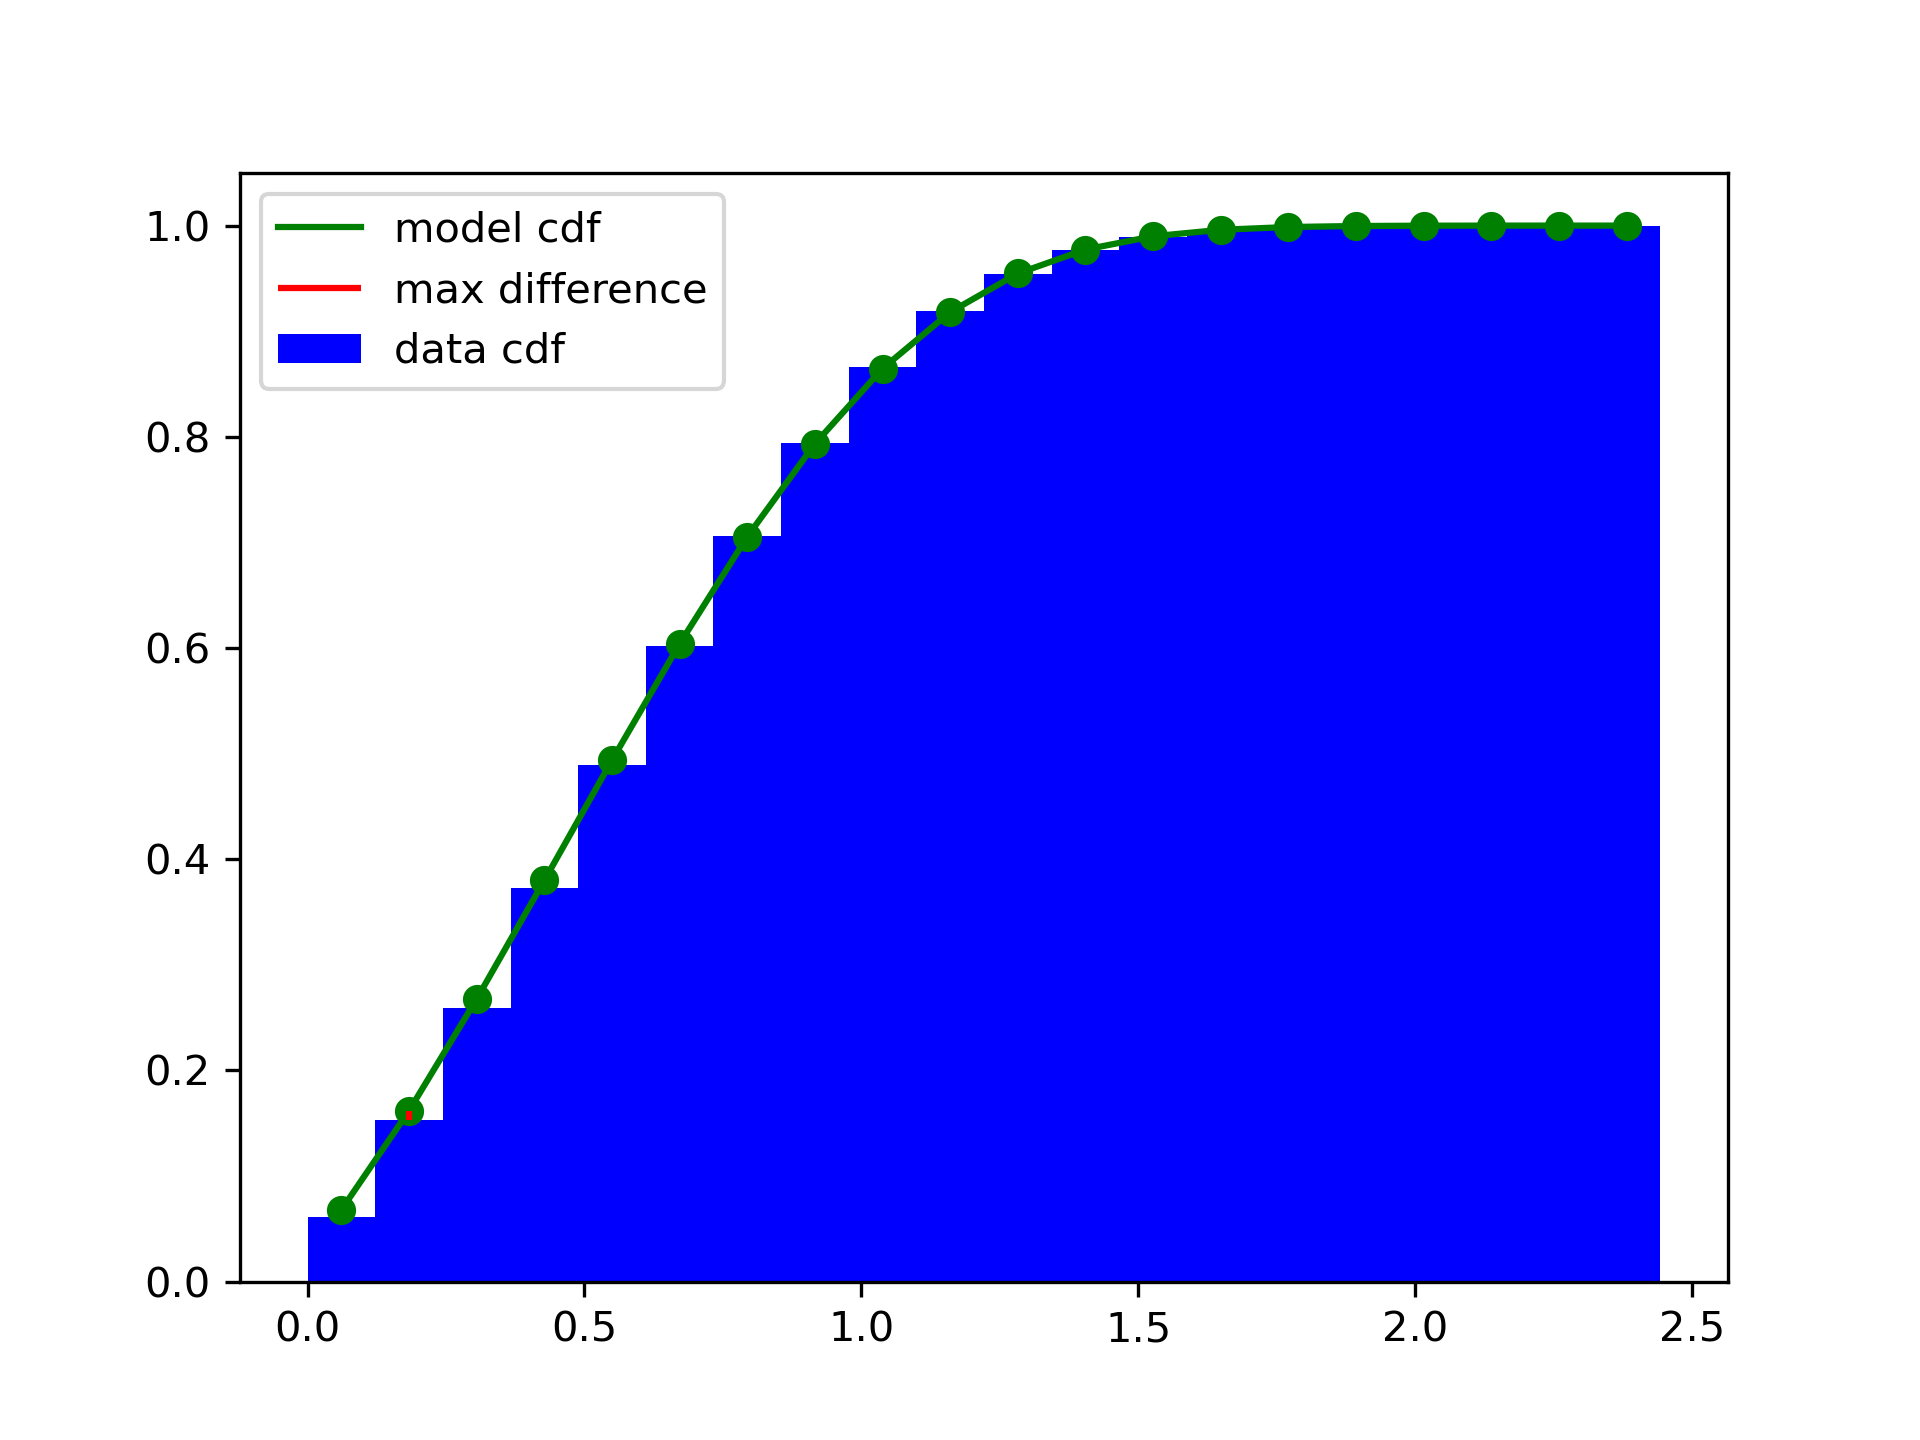
\includegraphics[width=.48\linewidth]{./plots/ks_chi_1.png}
  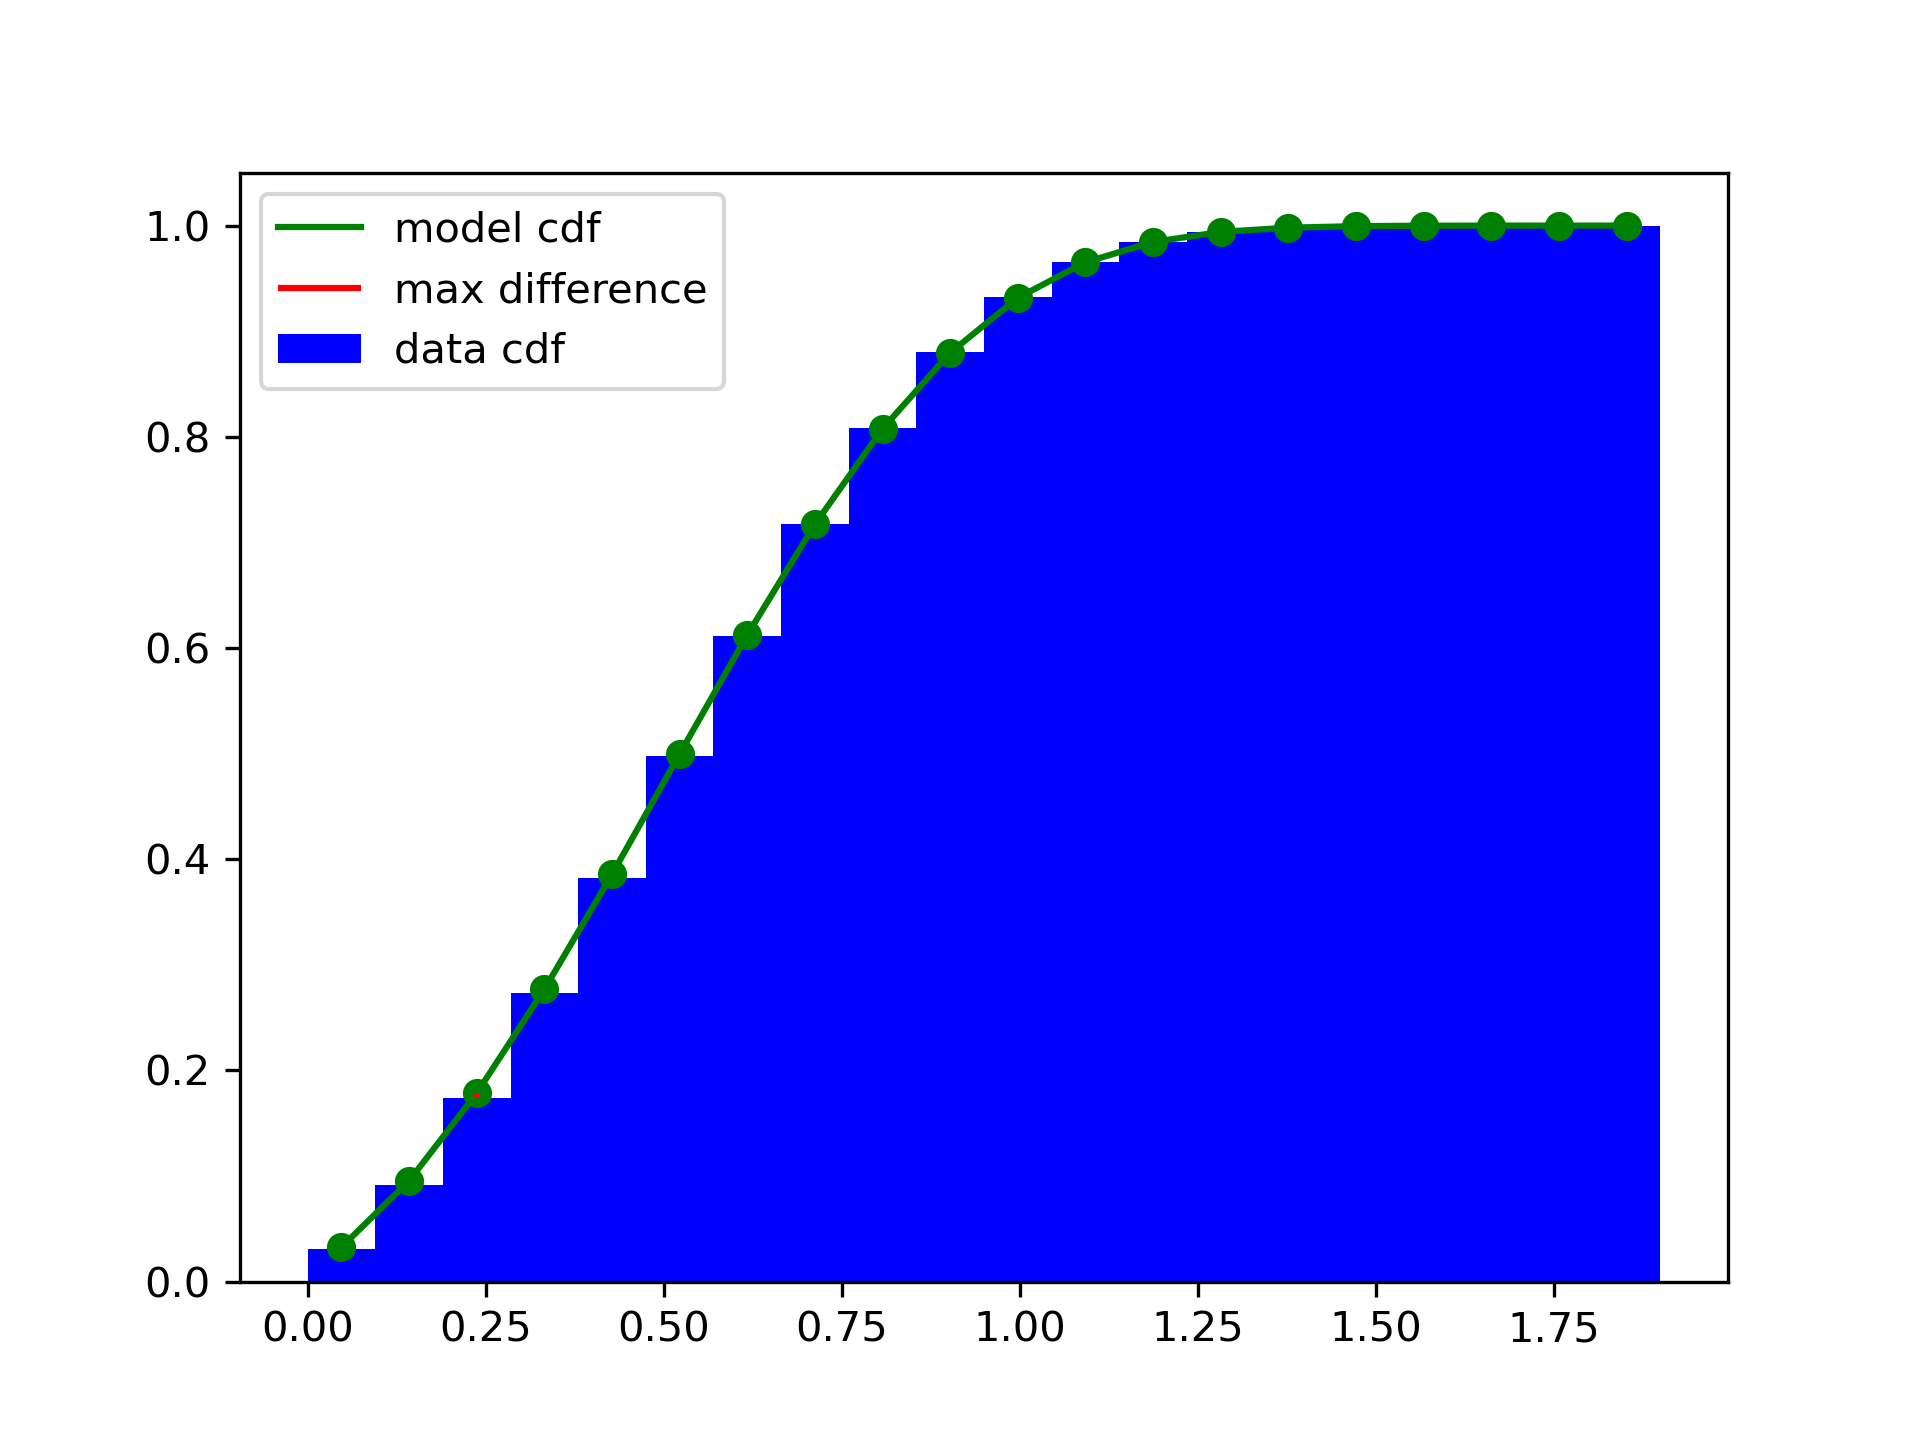
\includegraphics[width=.48\linewidth]{./plots/ks_chi_2.png}
  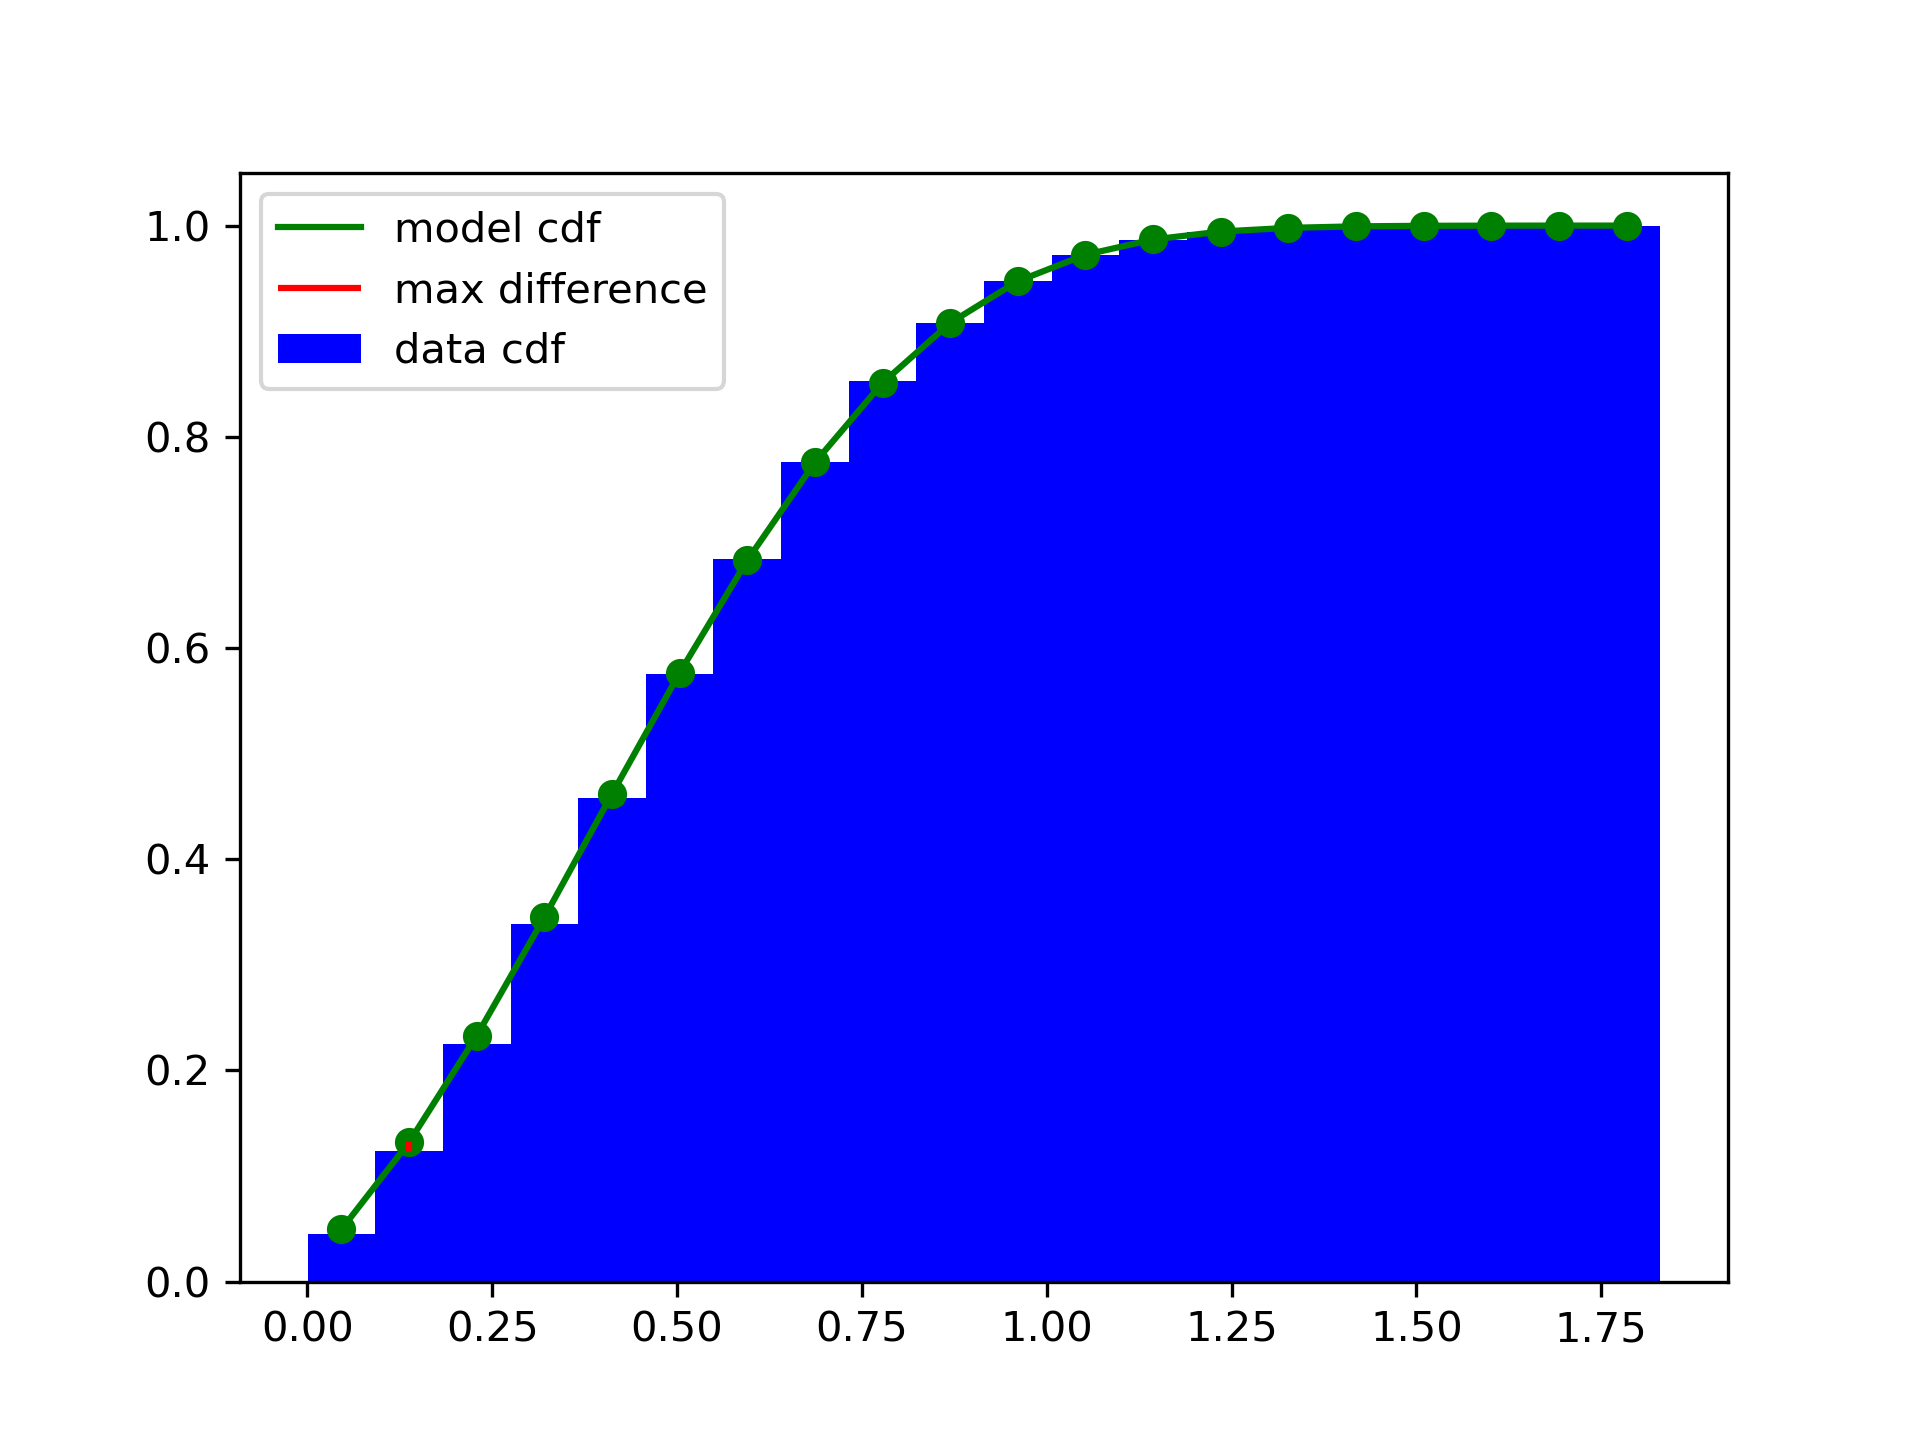
\includegraphics[width=.48\linewidth]{./plots/ks_chi_3.png}
  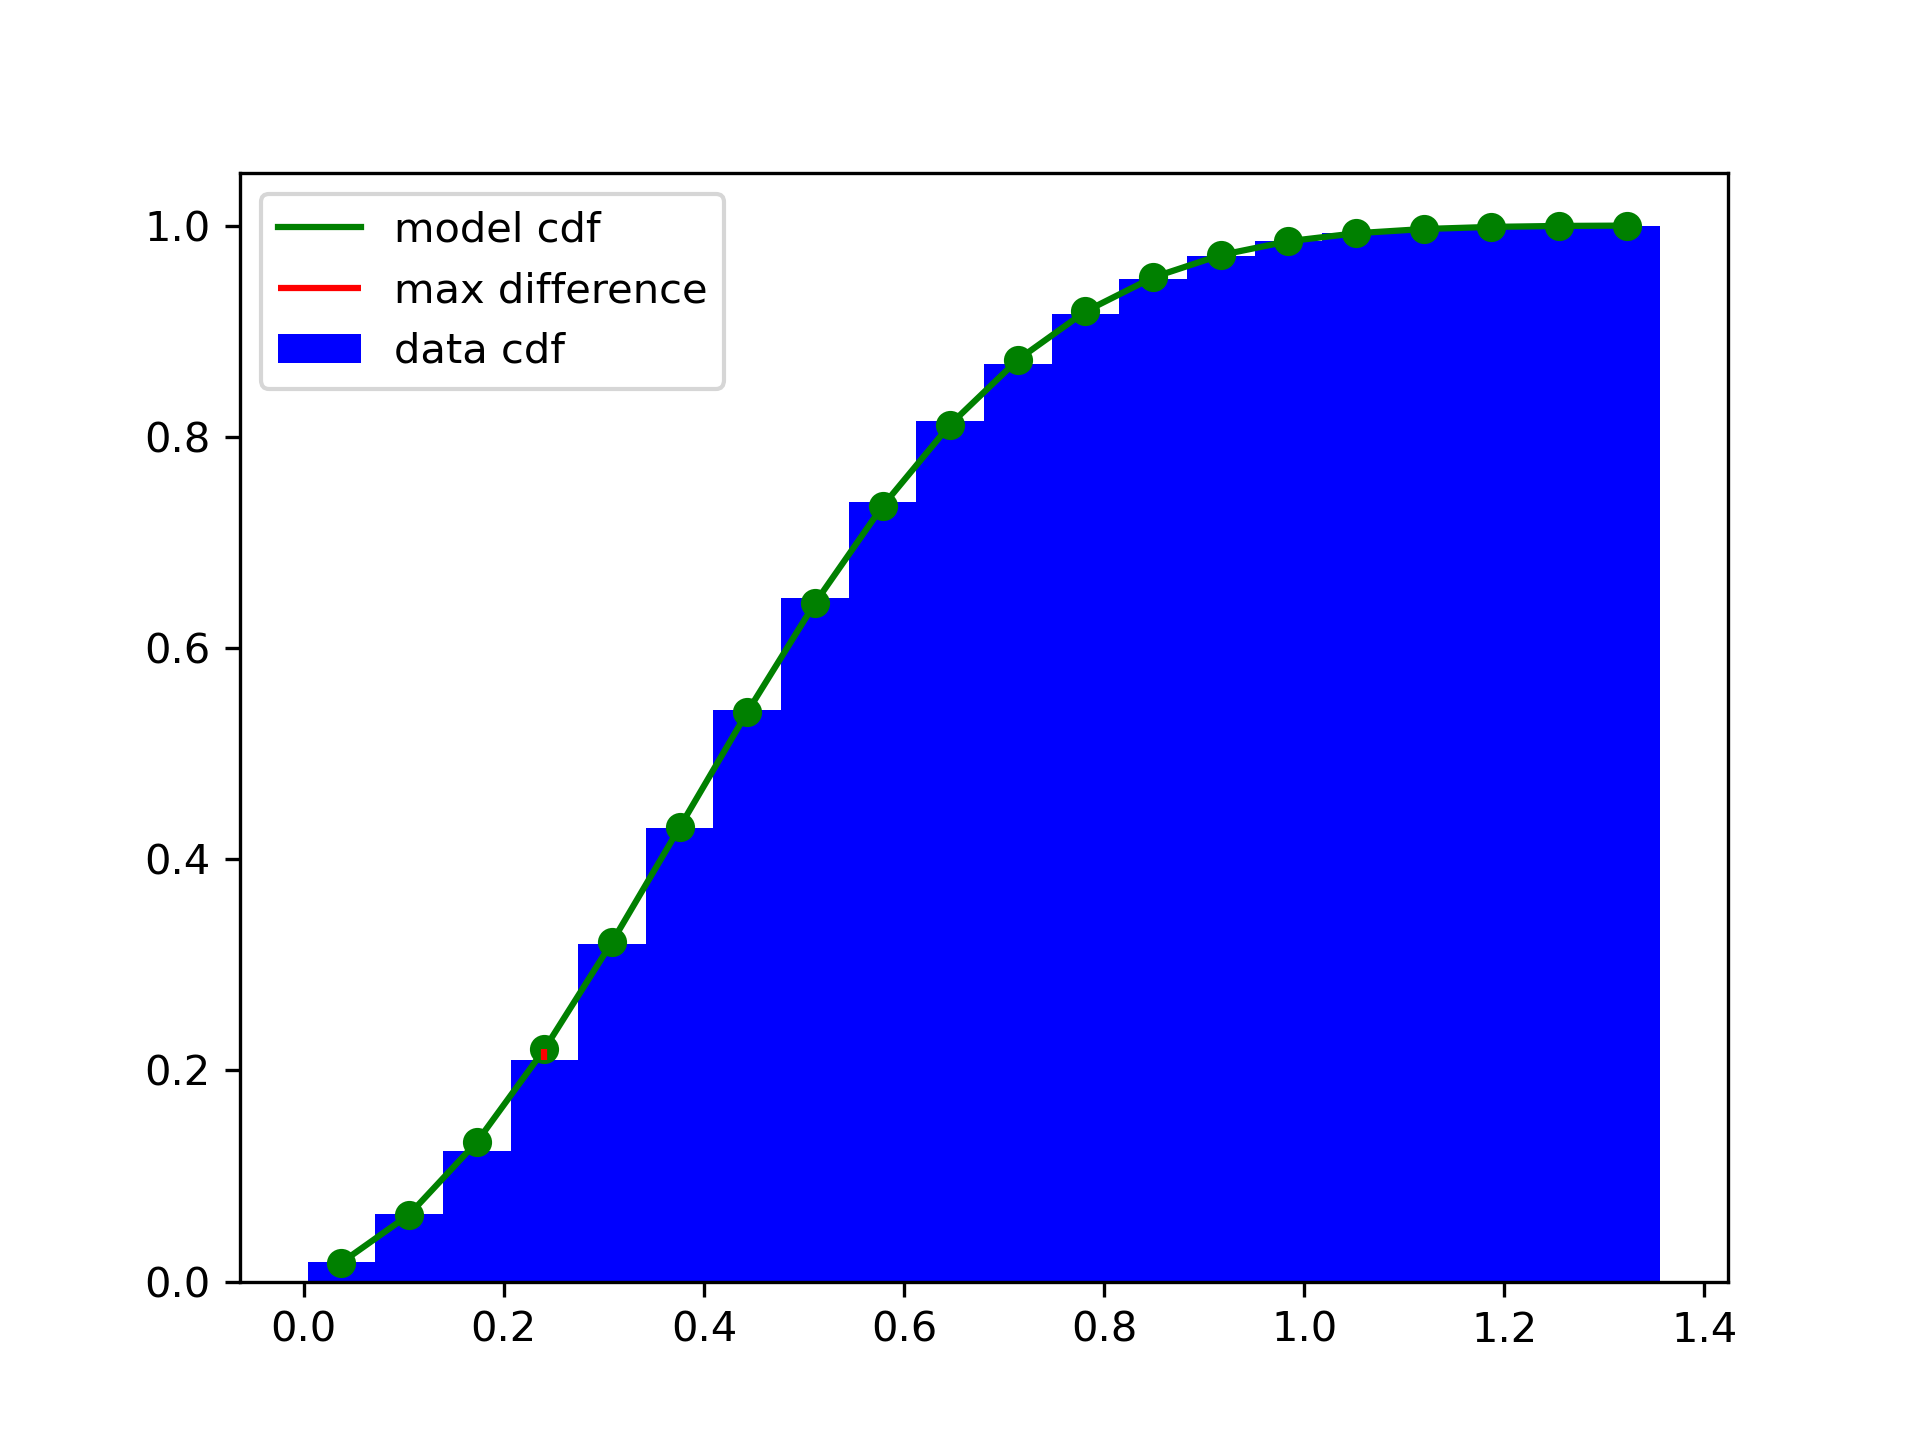
\includegraphics[width=.48\linewidth]{./plots/ks_chi_4.png}
  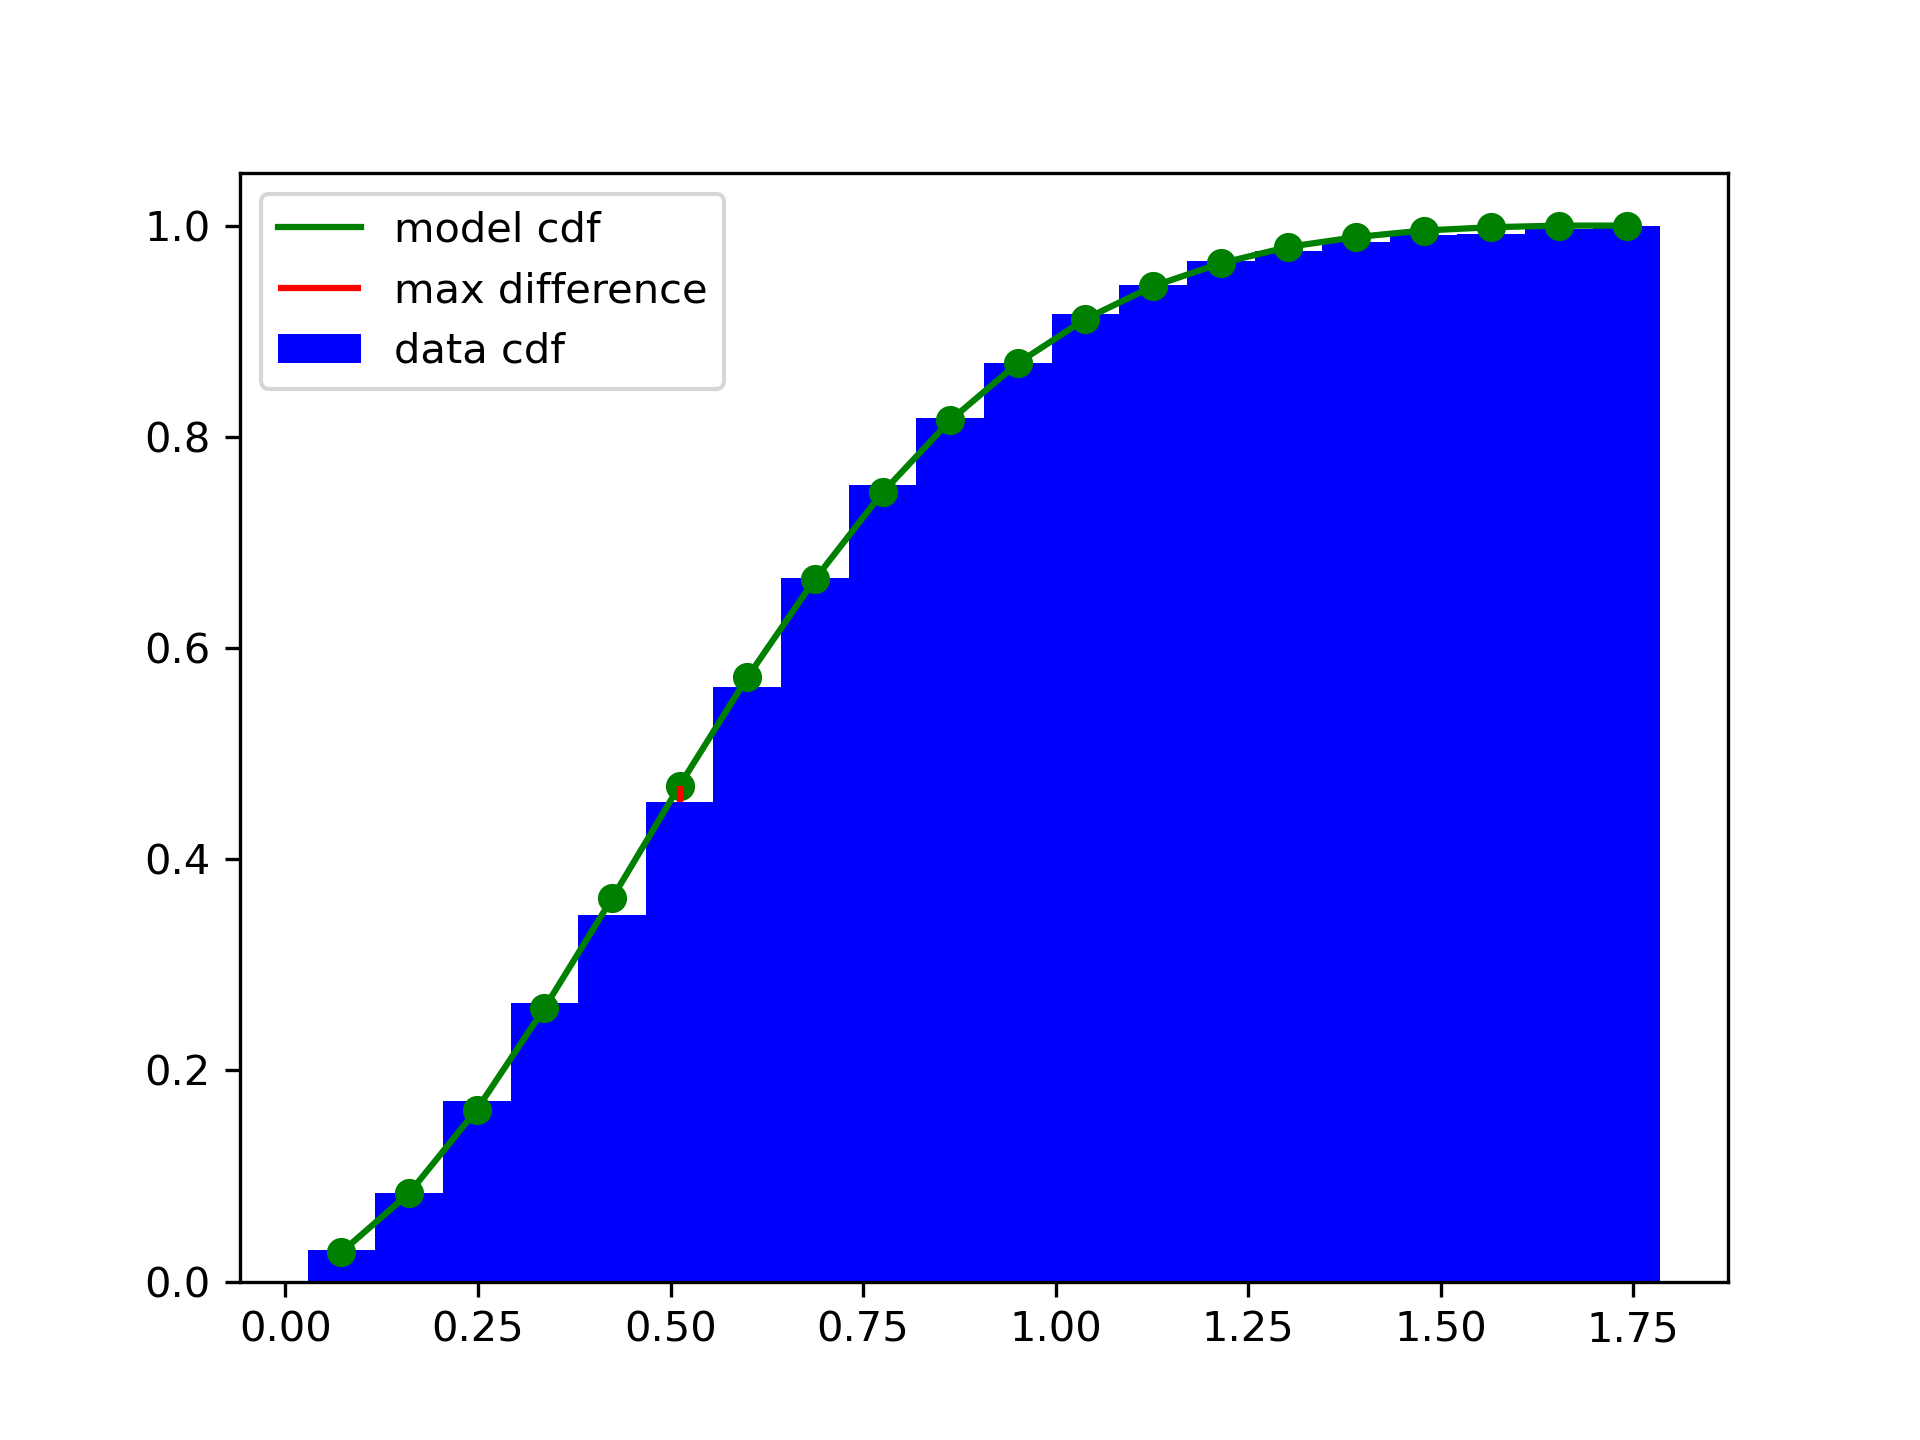
\includegraphics[width=.48\linewidth]{./plots/ks_chi_5.png}
  \caption{The cumulative distribution for both our binned data and the best-fit model using the $\chi^2$ minimization algorithm. We can see that there is a great match between them in all five cases as their maximum absolute difference is very small. This leads to a very high Q-value in the K-S test.}
  \label{fig:ks_chi}
\end{figure}

\begin{figure}[H]
  \centering
  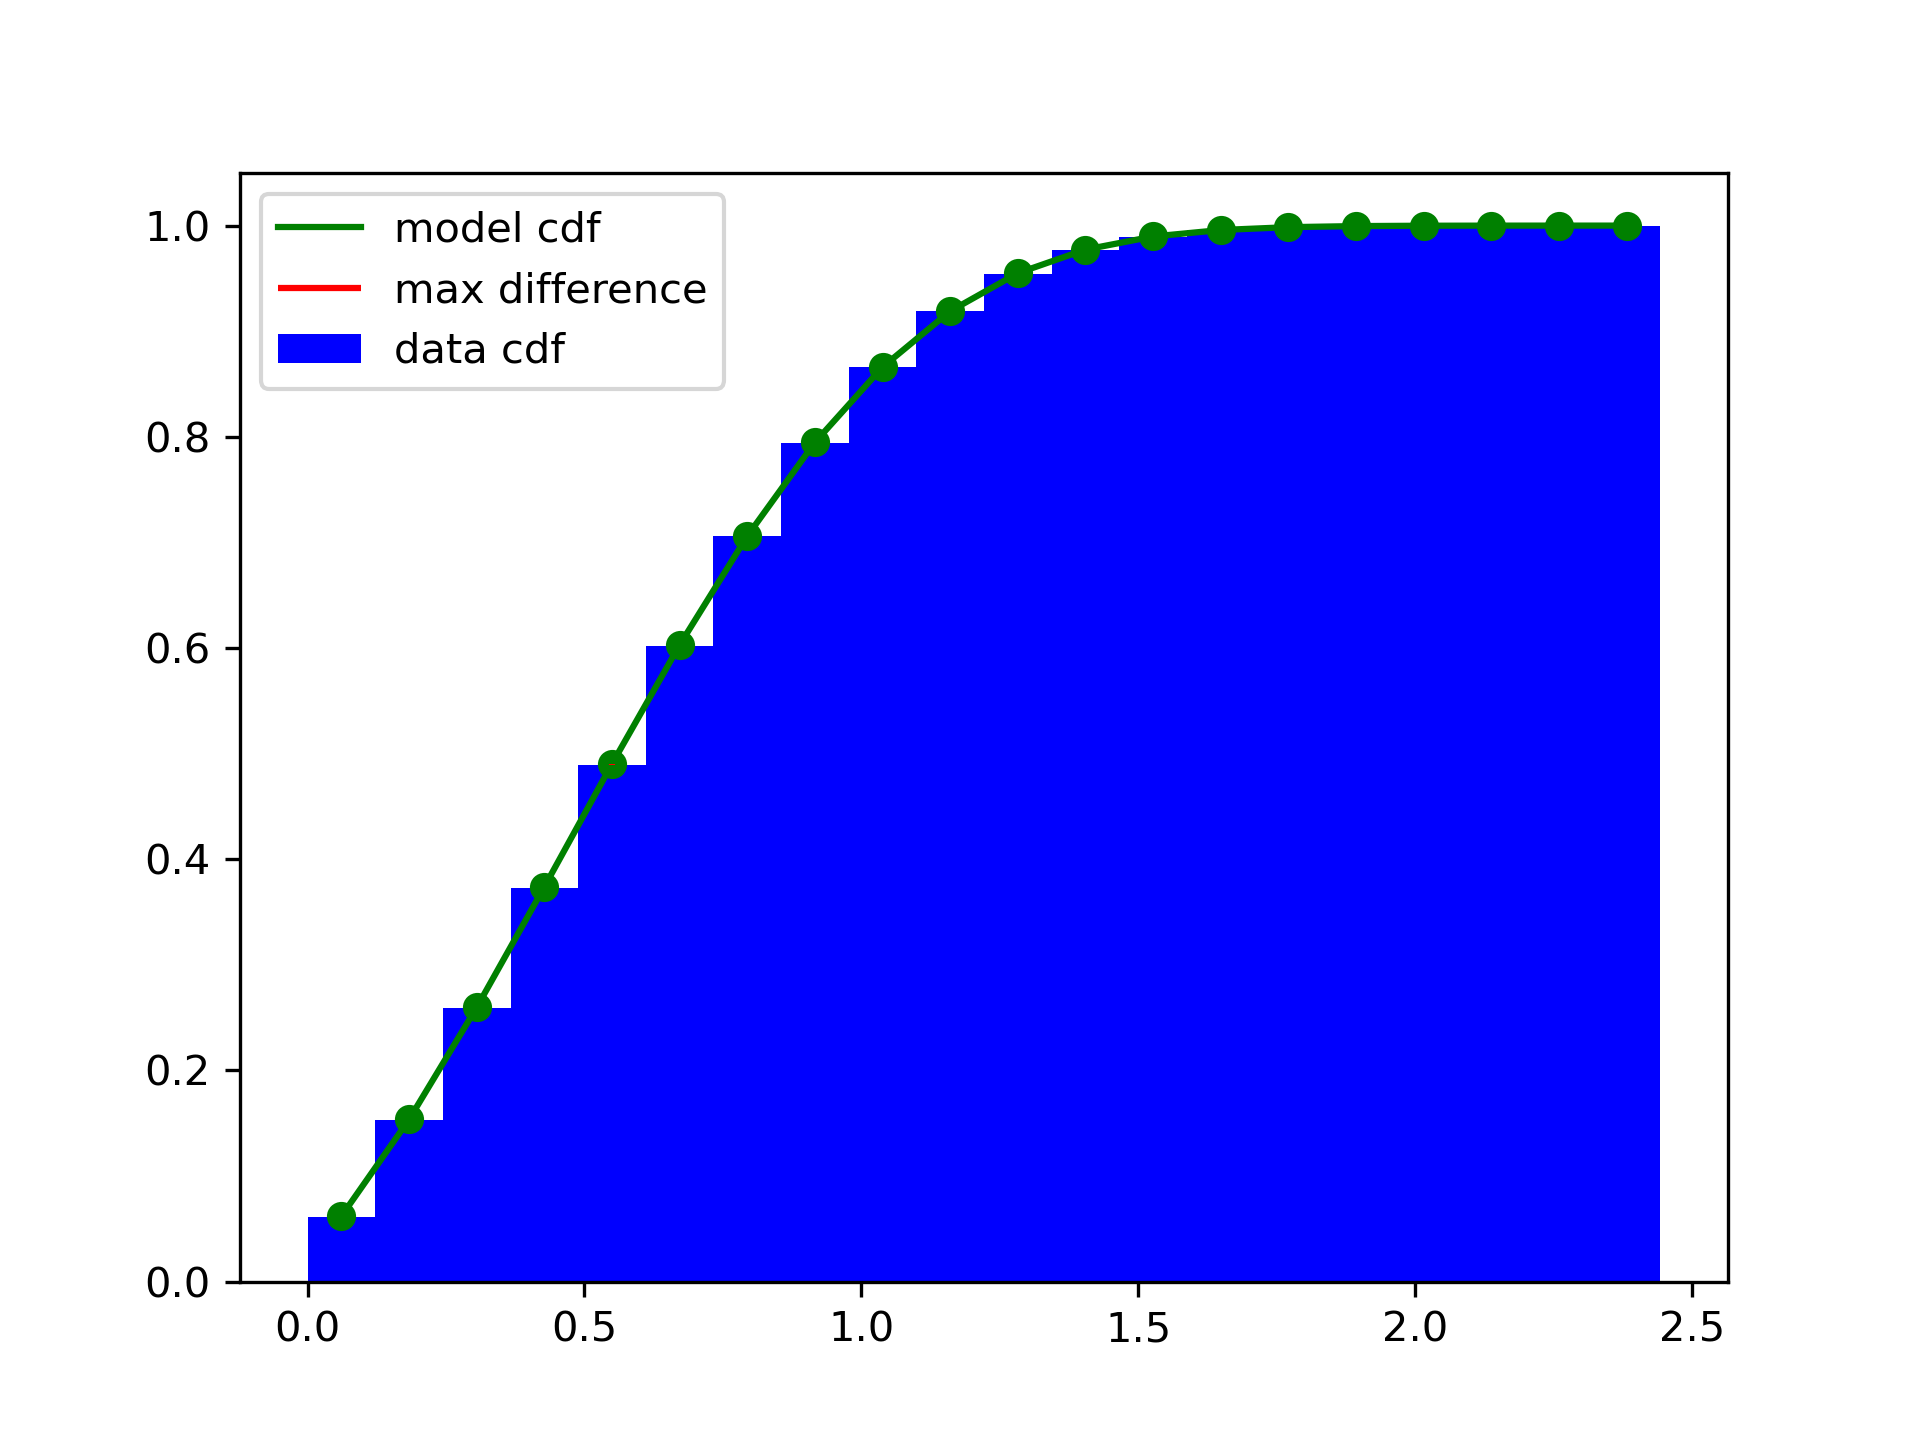
\includegraphics[width=.48\linewidth]{./plots/ks_pois_1.png}
  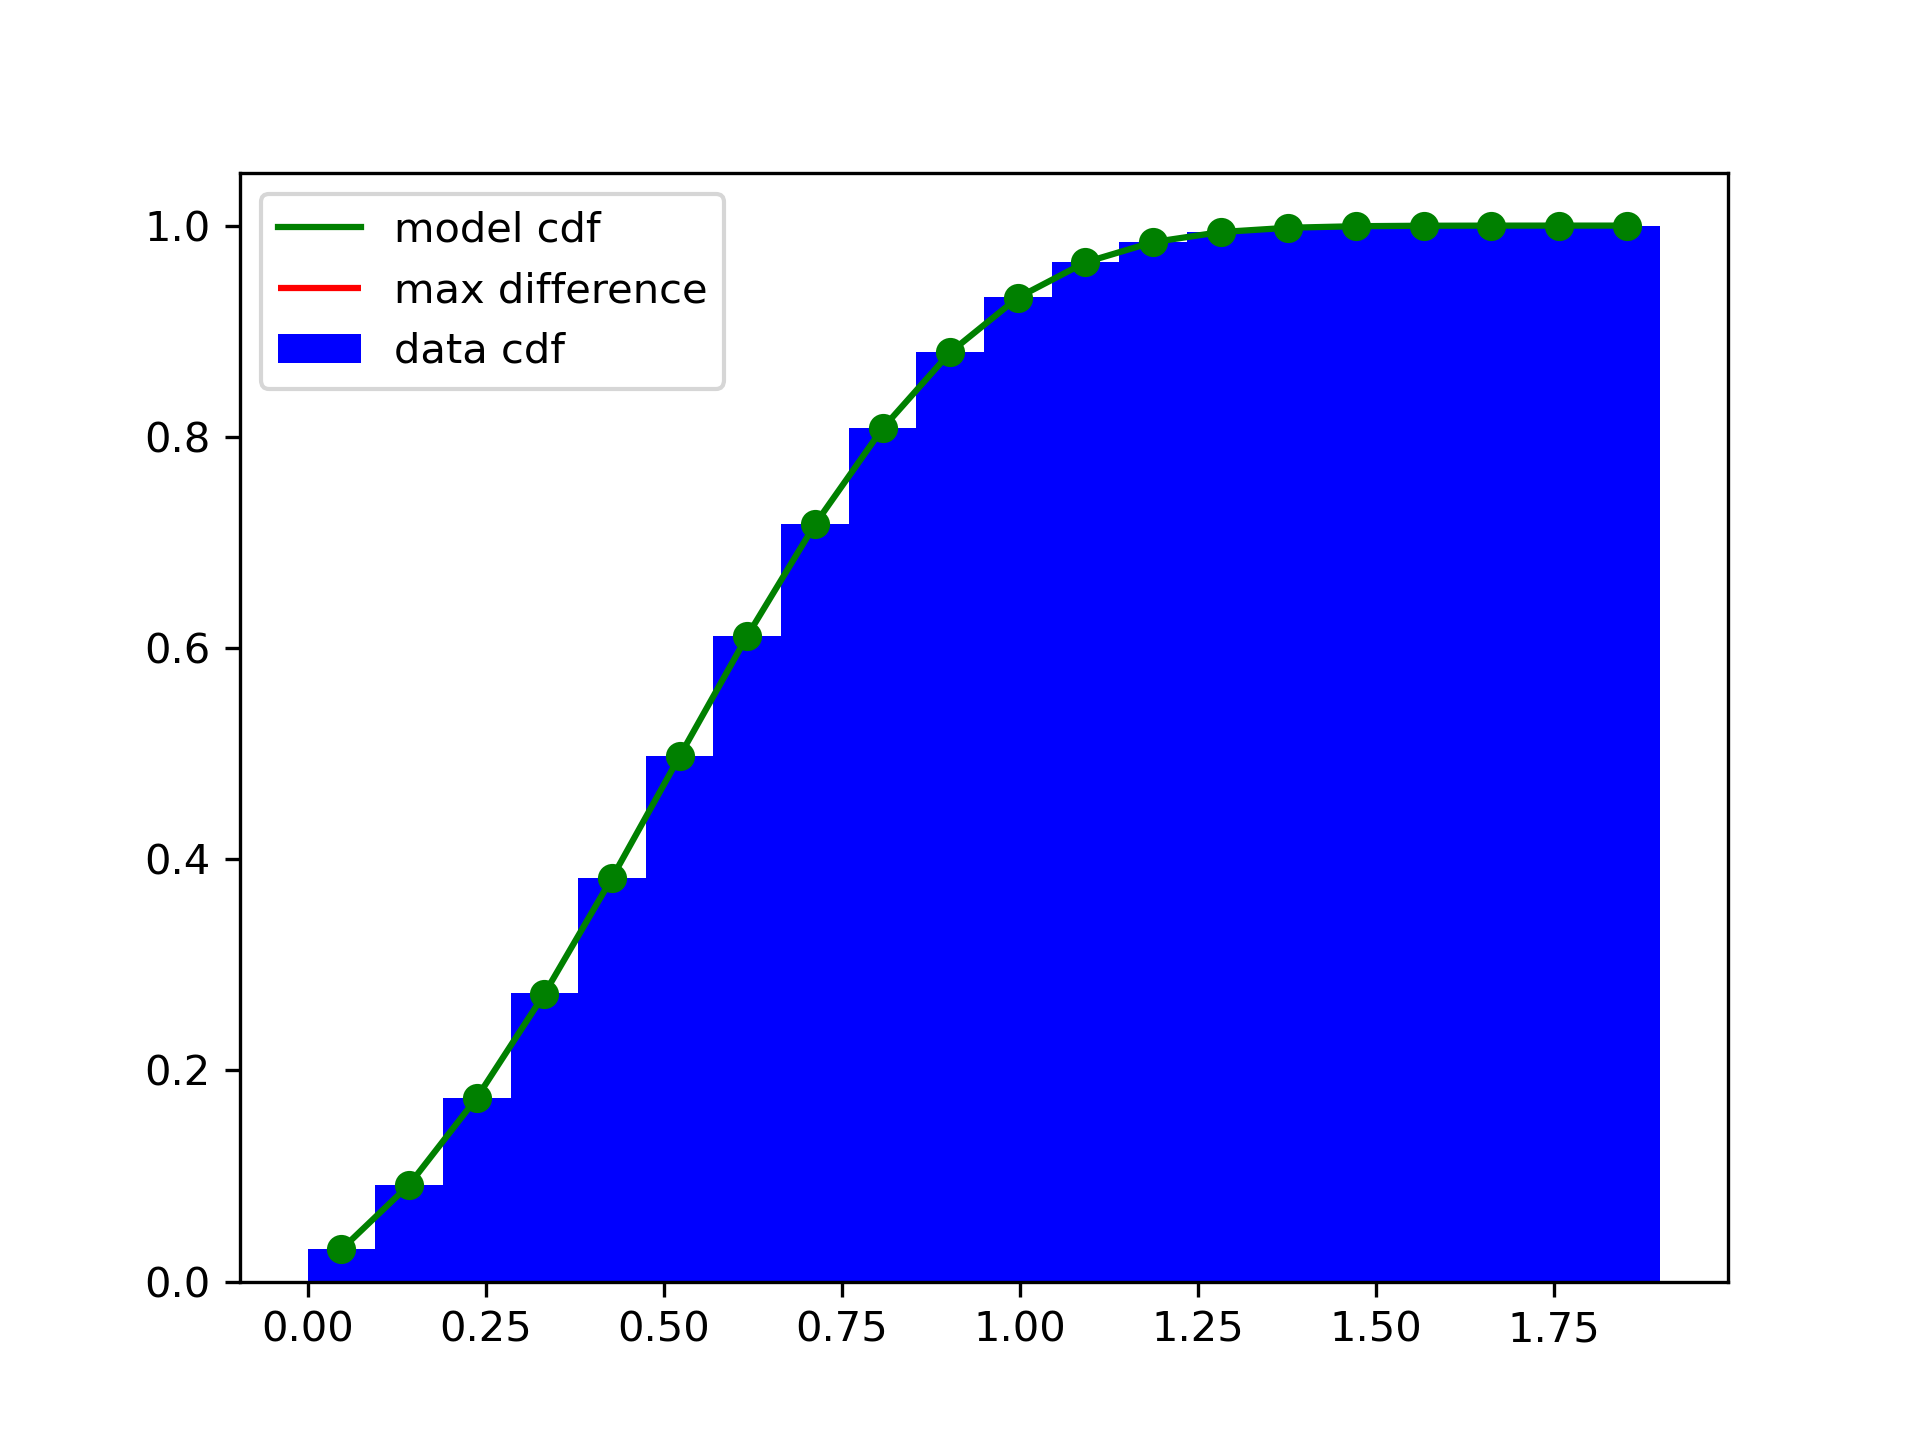
\includegraphics[width=.48\linewidth]{./plots/ks_pois_2.png}
  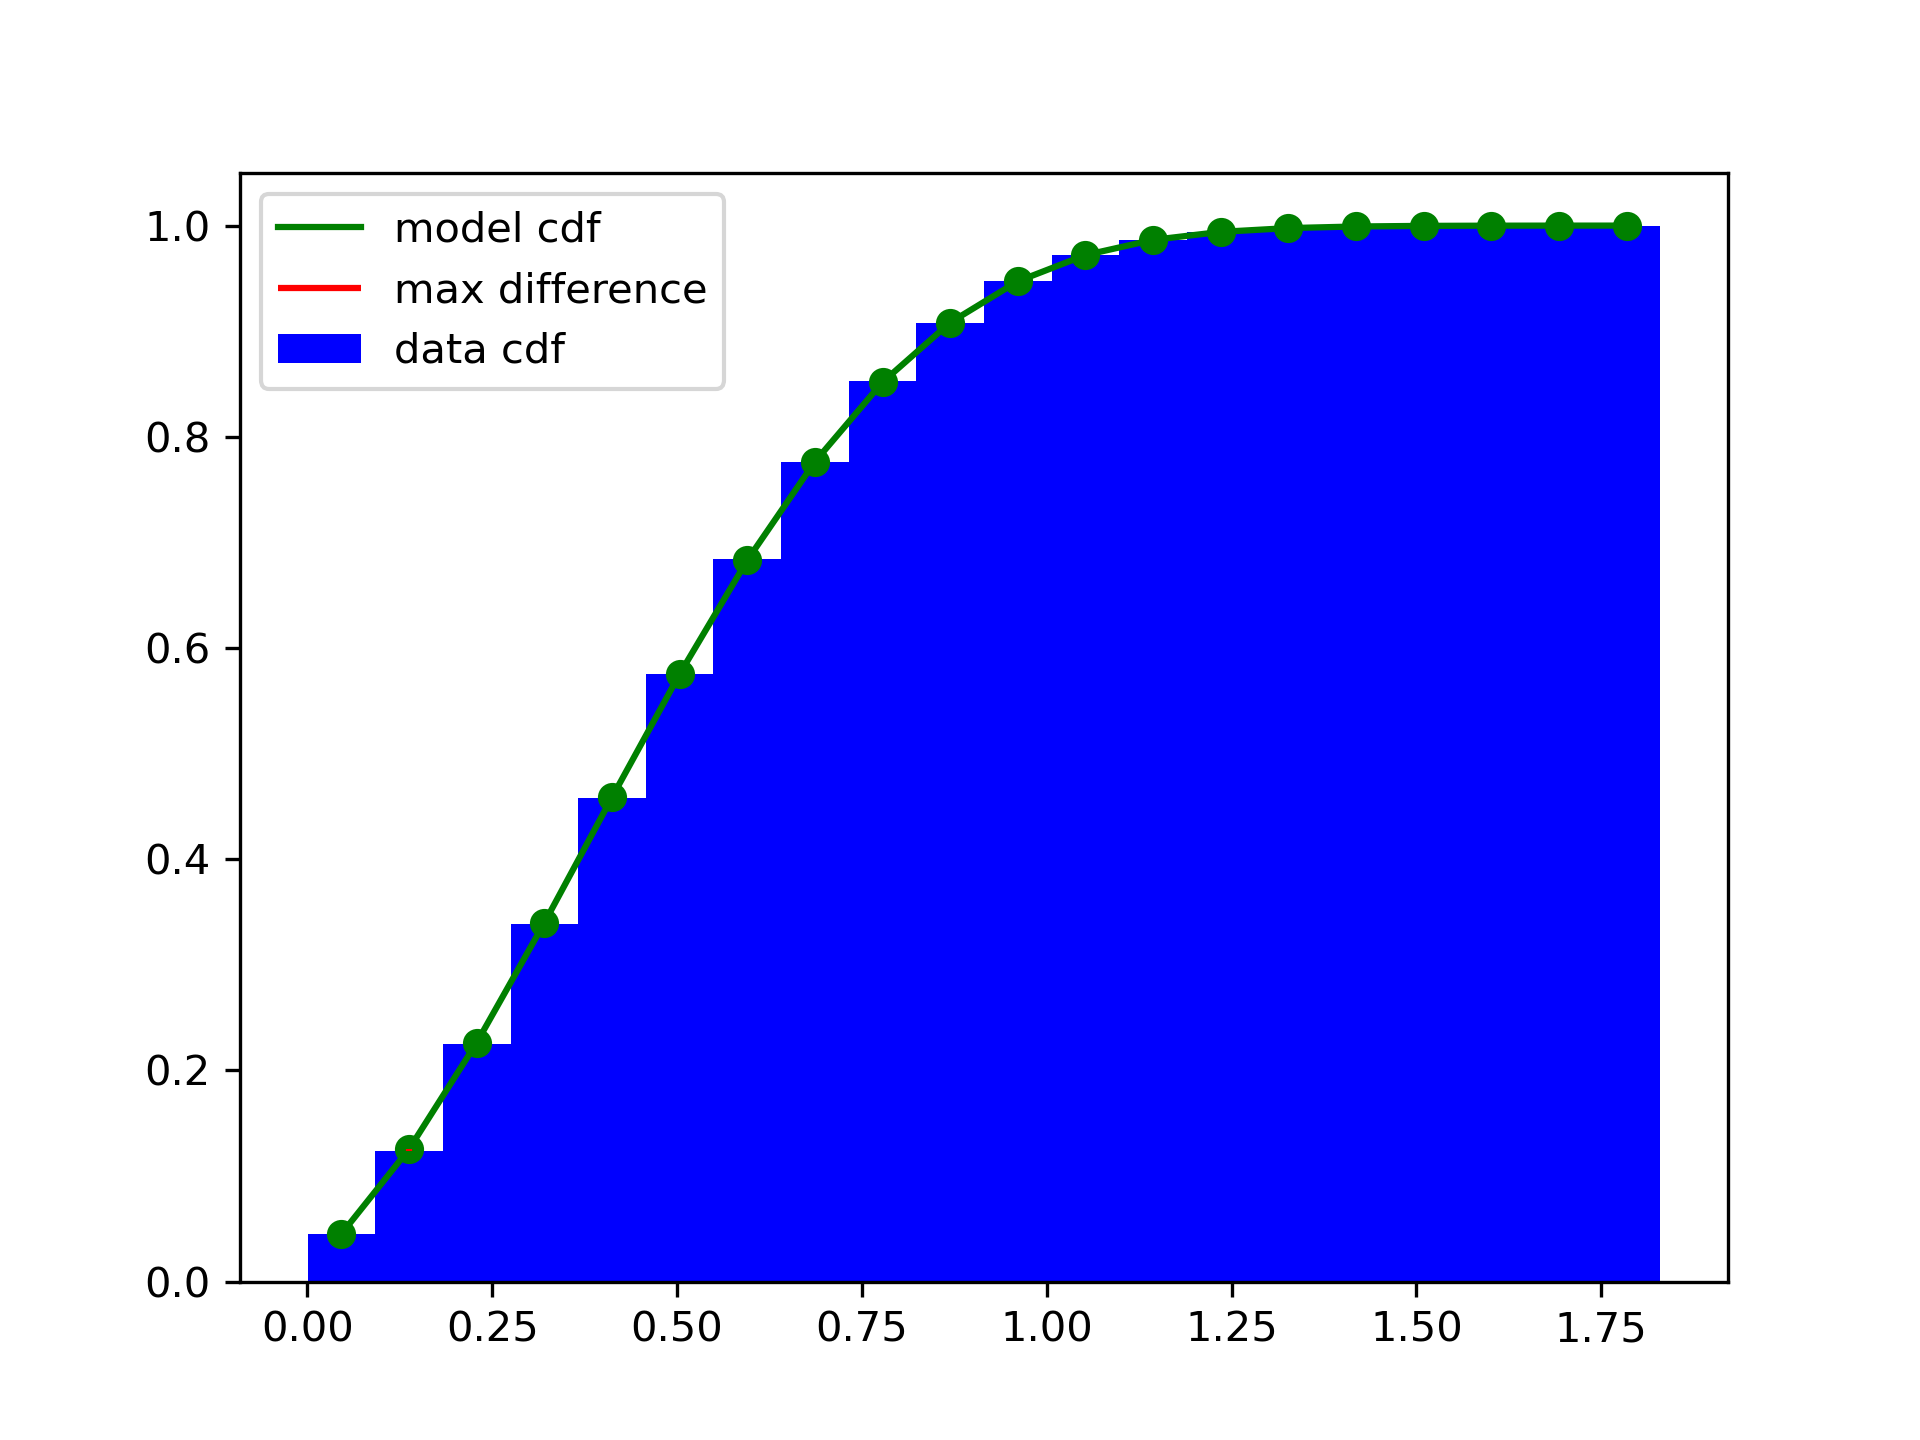
\includegraphics[width=.48\linewidth]{./plots/ks_pois_3.png}
  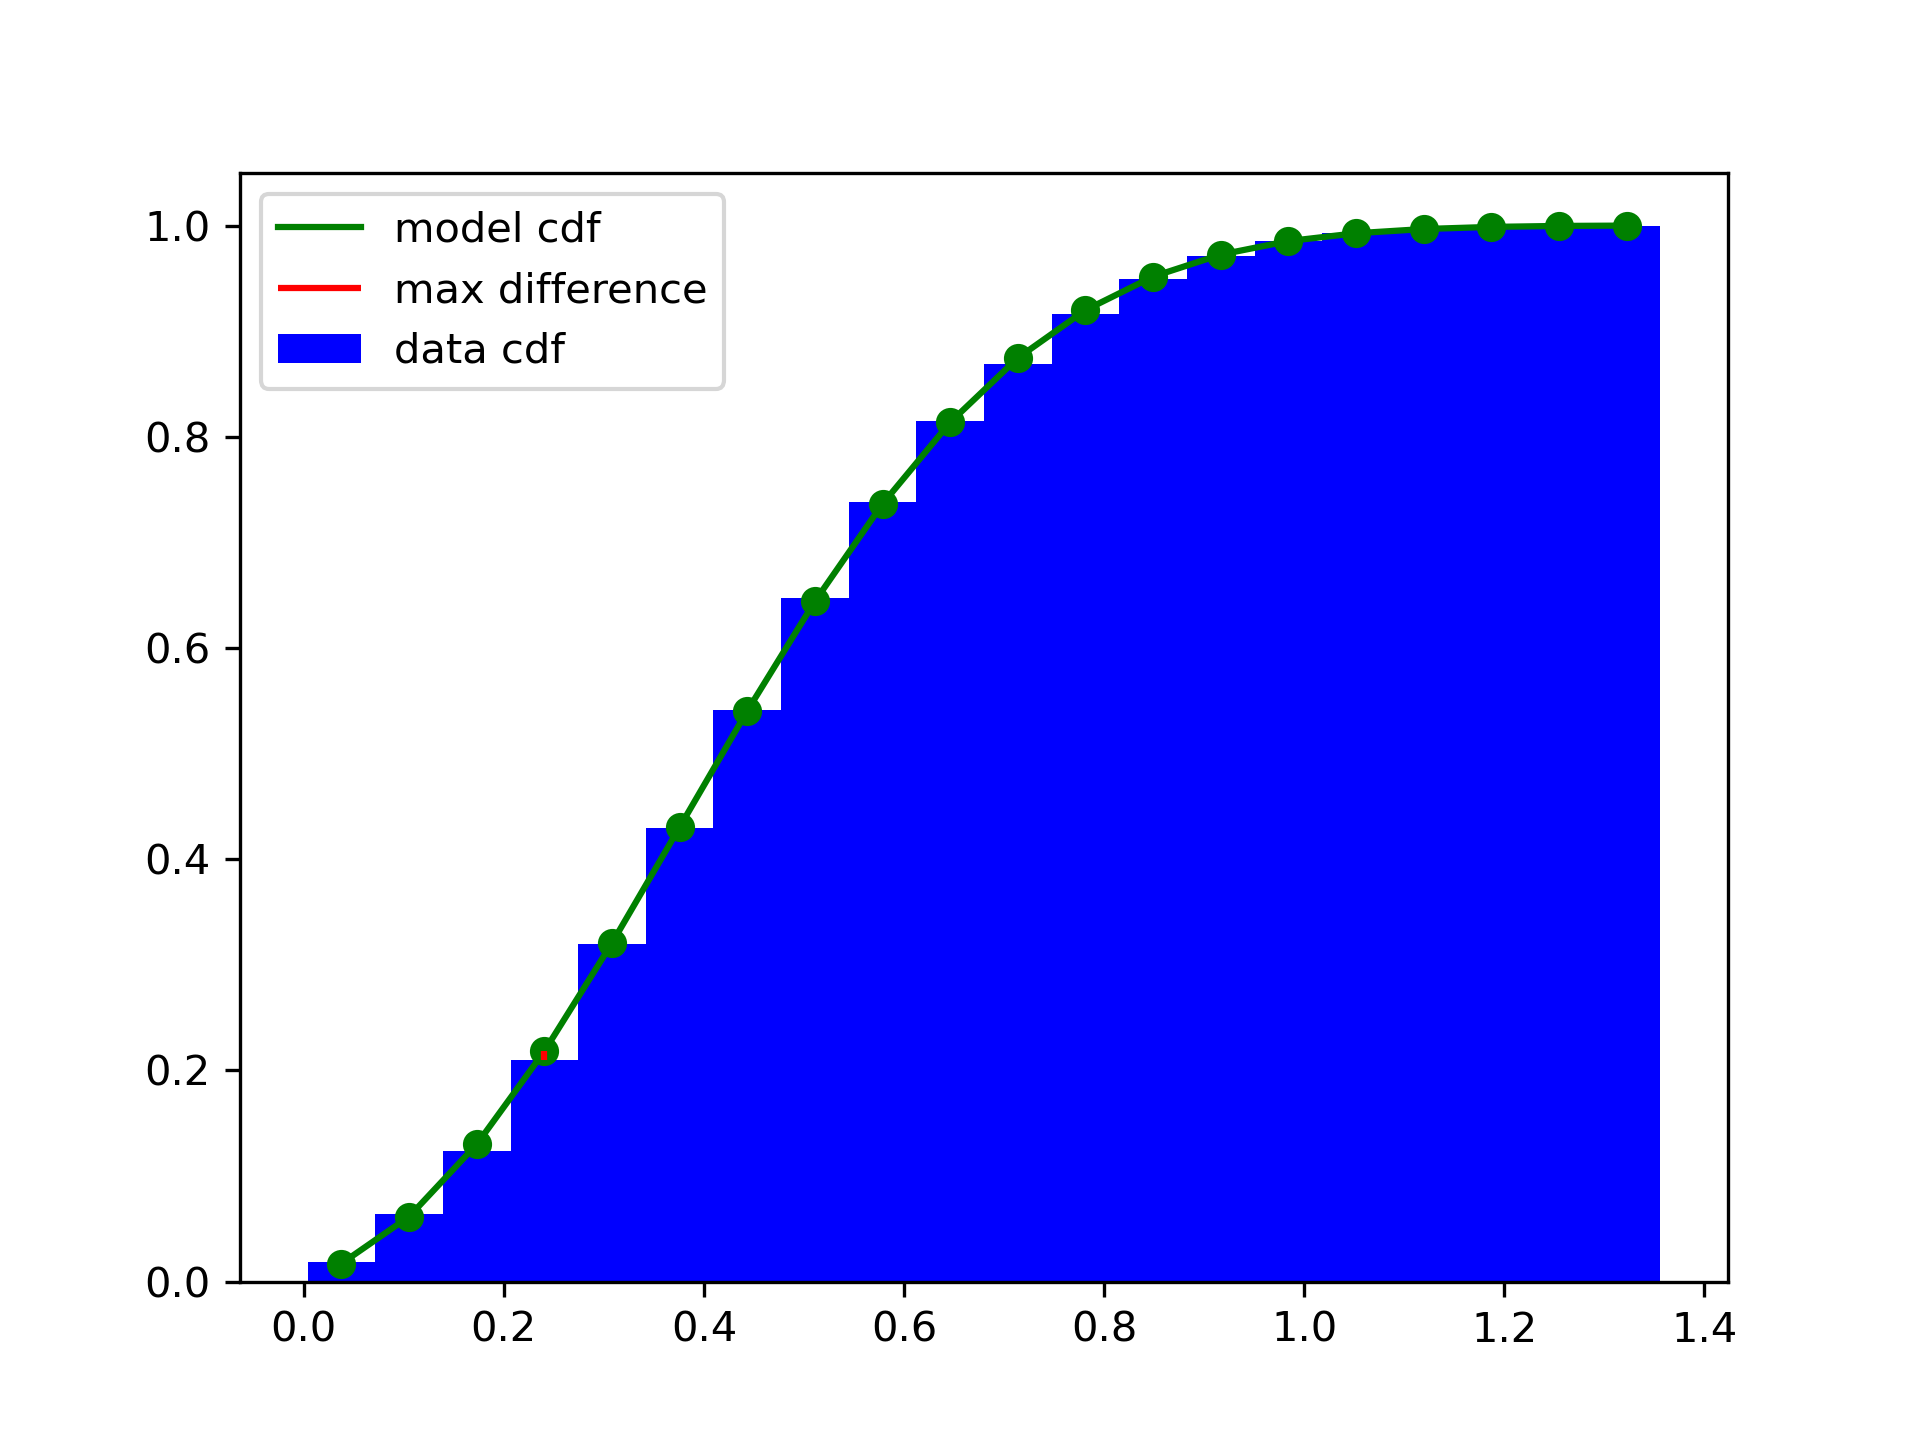
\includegraphics[width=.48\linewidth]{./plots/ks_pois_4.png}
  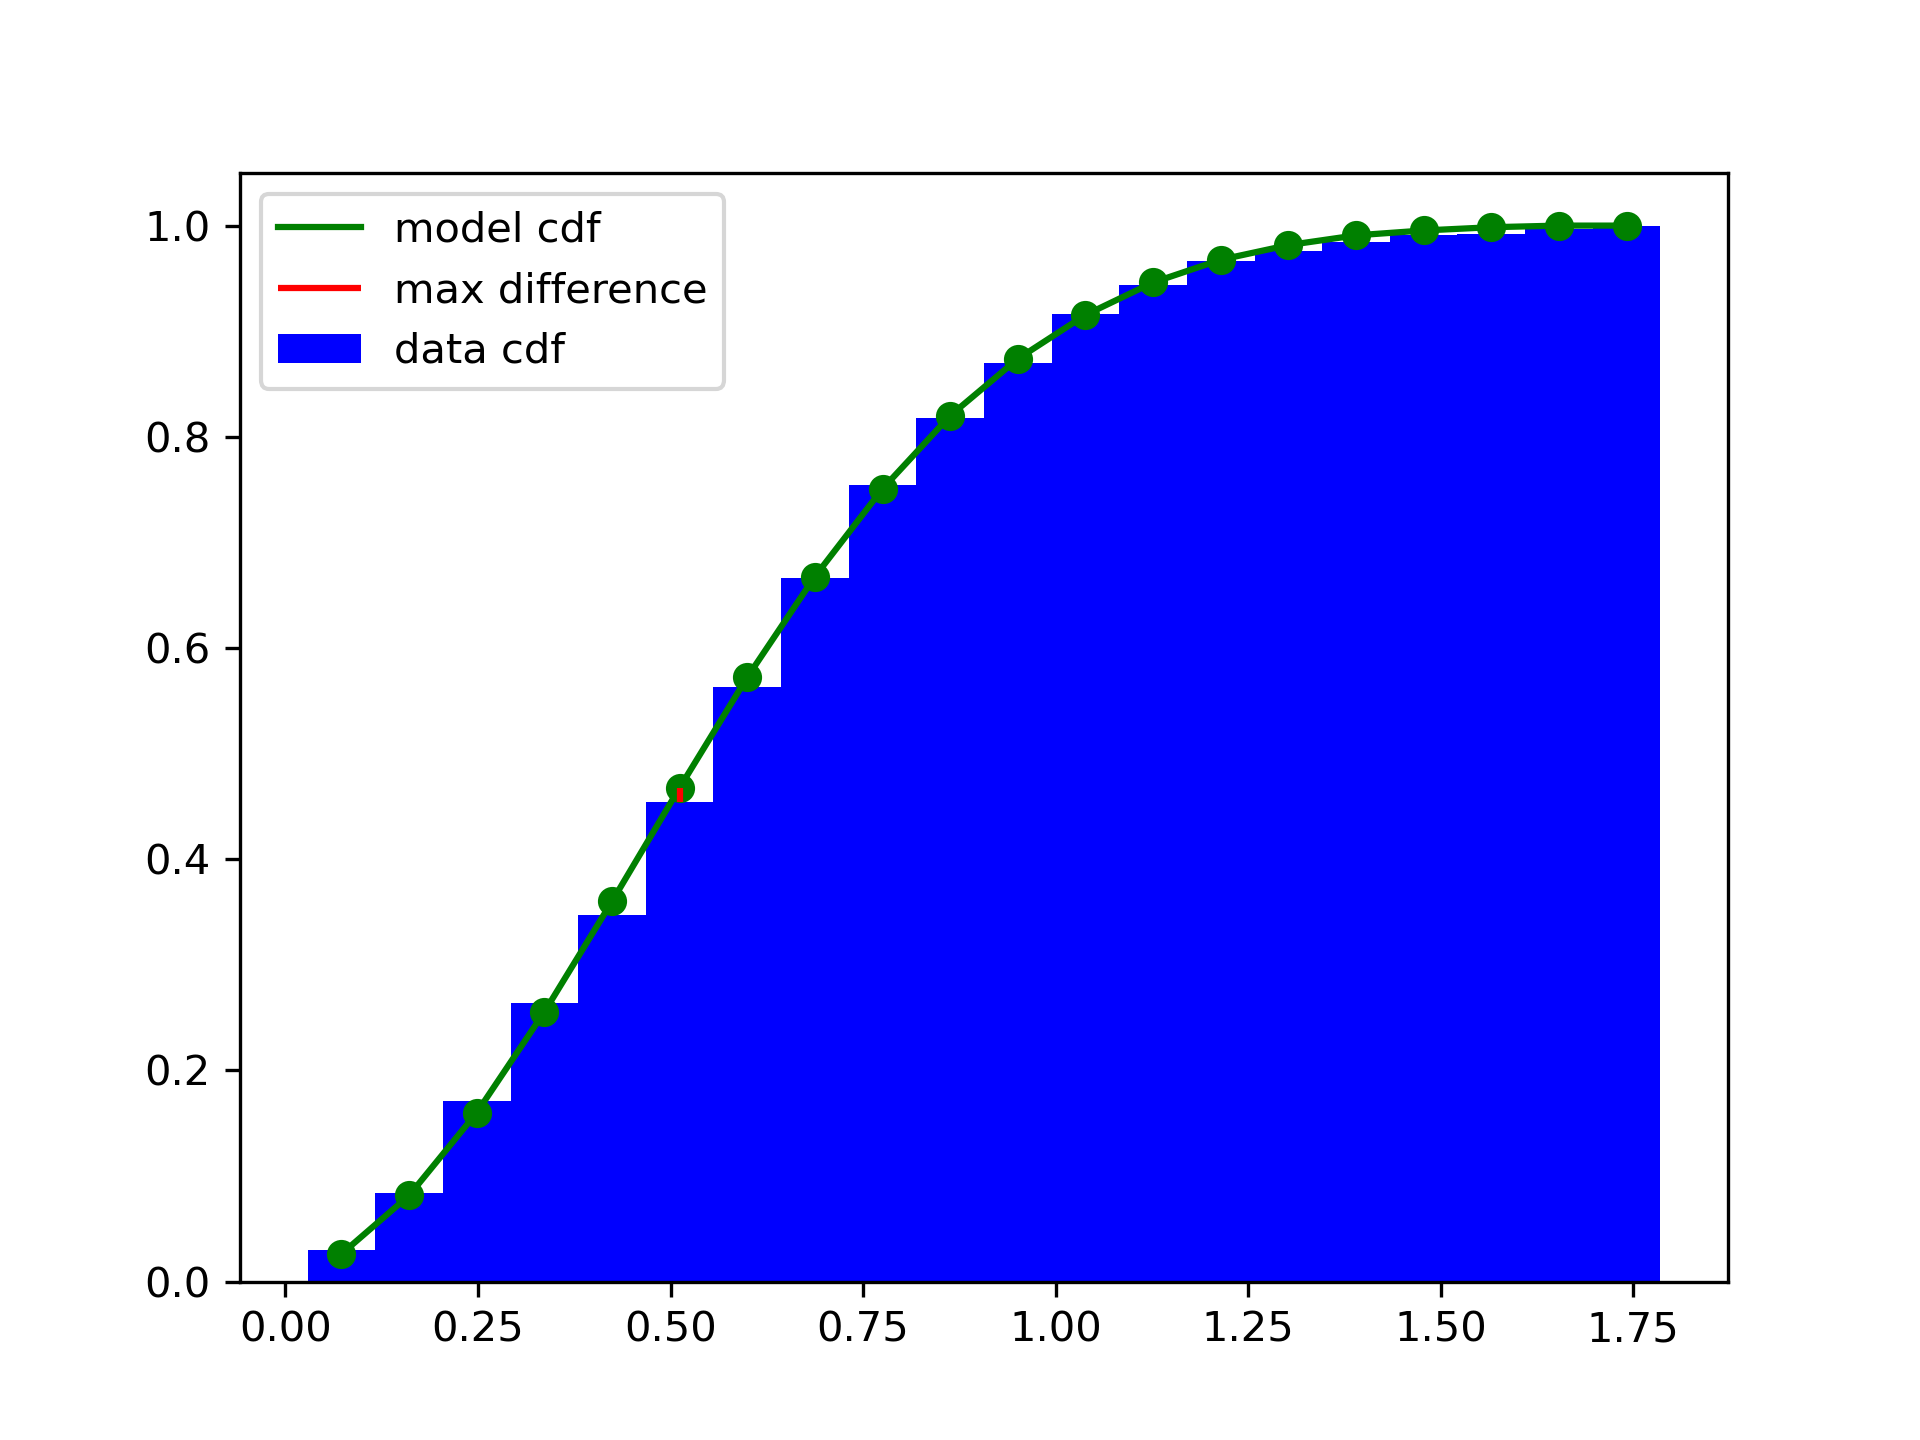
\includegraphics[width=.48\linewidth]{./plots/ks_pois_5.png}
  \caption{The cumulative distribution for both our binned data and the best-fit model. The models were fit by minimizing the Poisson loglikelihood. We can see that there is a great match between them in all five cases as their maximum absolute difference is very small. This leads to a very high Q-value in the K-S test.}
  \label{fig:ks_pois}
\end{figure}

\end{document}
